\chapter{Численное моделирование аттракторов внутренних гравитационных волн}
\label{cha:Simulation}

В данной главе рассматриваются три принципиально различных подхода к моделированию аттракторов внутренних волн.

Первый, метод спектральных элементов\cite{Patera1984}. Результаты полученные при помощи метода спектральных элементов были достаточно близки к результатам натурных экспериментов\cite{Brouzet2016,Brouzet_2016}. Недостатком метода является отсутсвие реализаций с открытым исходным кодом позволяющие встроить дополнительные физические модели и проводить расчеты на сложной геометрии приближенной к реальной топологии океанического дна.

Второй метод, метод конечных объемов на основе классических уравнений Навье-Стокса в приближении Буссинеска, качественно воспроизводит явление аттракторов, но количественно имеет большую погрешность. Однако его многочисленные реализации, в том числе и с открытым исходным кодом, предоставляют возможность для построения сложных сеток и геометрий. Также эти инструменты снабжены возможностями добавлять собственные реализации физических моделей, граничных условий и утилит. 

Третий способ также основан на методе конечного объема и сохраняет его преимущества, но он представляет собой реализацию квазигидродинамических уравнений\cite{ElizarBook}. Такой подход, еще называемый регуляризованным, обеспечивает точность выше, чем у реализации классической системы уравнений Навье-Стокса.

В работе рассматриваются различные конфигурации расчетной области (Рис. \ref{fig:dominleft},\ref{fig:domainup}).

\begin{figure}[!ht]
        \centering
          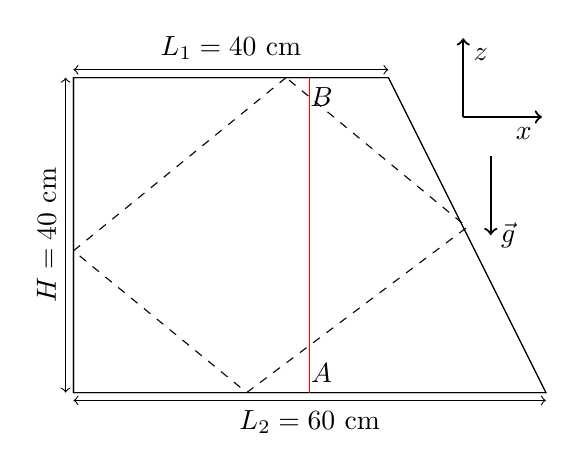
\begin{tikzpicture}[scale=1.0, z={(-.707,-.5)}]
            \draw (0,0,0) -- (6,0,0) -- (4,4,0)--(0,4,0) --cycle;
            \draw (0,0,0)     -- (6,0,0)   -- (4,4,0)   -- (0,4,0)    -- cycle;
            \draw[style = dashed] (2.7,4,0)   -- (0,1.8,0) -- (2.2,0,0) -- (5,2.1,0)-- cycle;
            %\draw[style = dashed] (0,0.985,0) -- (3.3,4,0) -- (4.5,3,0) -- (1.1,0,0)  -- cycle;

            \draw[<->] (-0.1,0) --node[above,rotate=90] {$H = 40$ cm} (-0.1,4);
            \draw[<->] (0,-0.1,0) --node[below,] {$L_2 = 60$ cm} (6,-0.1,0);
            \draw[<->] (0,4.1,0) --node[above,] {$L_1 = 40$ cm} (4,4.1,0);

            \draw[color=red] (3.0,0)--(3.0,4.0);
            
            \draw (3.15,0) node[above] {$A$};
            \draw (3.15,4.0) node[below] {$B$};

            \draw[thick,->] (4.95,3.5,0) -- (5.95,3.5,0) node[anchor=north east]{$x$};
            \draw[thick,->] (4.95,3.5,0) -- (4.95,4.5,0) node[anchor=north west]{$z$};
            \draw[thick,->] (5.3,3,0) -- (5.3,2,0) node[anchor=west]{$\vec{g}$};
          \end{tikzpicture}
          \caption{Вычислительная область для аттракторов внутренних волн, красным показана линия пробы, пунктиром показана предполагаемая форма аттрактора}
          \label{fig:dominleft}
\end{figure}

\begin{figure}[!ht]
    \centering
    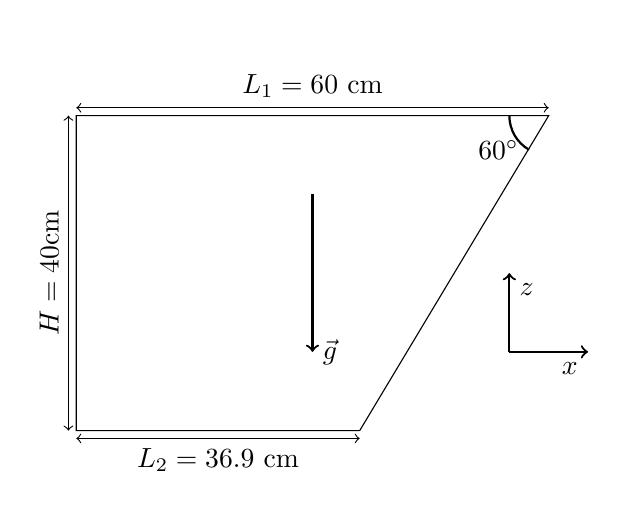
\begin{tikzpicture}[scale=1, z={(-.707,-.5)}]
    \draw (3.6,0,0) -- (0,0,0) -- (0,4,0)--(6,4,0)--(3.6,0,0);
    %\draw (3.6,0,0) -- (3.6,0,-1) -- (6,4,-1) -- (6,4,0) -- cycle;
    %\draw (6,4,0) -- (0,4,0) -- (0,4,-1) -- (6,4,-1);
    \draw (-0.5,2,0) node{};
    \draw (4.1,-.2,-1.5) node{};
    \draw (3.5,5,0) node{};
    \draw[<->] (-0.1,0) --node[above,rotate=90] {$H = 40$cm} (-0.1,4);
    \draw[<->] (0,4.1,0) --node[above,] {$L_1 = 60$ cm} (6,4.1,0);
    \draw[<->] (0,-0.1,0) --node[below,] {$L_2=36.9$ cm} (3.6,-0.1,0);
    \draw [black, thick] (5.5,4) arc [start angle=180, end angle=240, radius=0.5cm]
        node [left] {$60^\circ$};
    \draw[thick,->] (5.5,1,0) -- (6.5,1,0) node[anchor=north east]{$x$};
    \draw[thick,->] (5.5,1,0) -- (5.5,2,0) node[anchor=north west]{$z$};
    \draw[thick,->] (3,3,0) -- (3,1,0) node[anchor=west]{$\vec{g}$};
    \end{tikzpicture}
    \caption{Конфигурация вычислительной области для аттрактора внутренних гравитационных волн}
    \label{fig:domainup}
\end{figure}

Принципиальной разницы в этих двух вариантах нет в первом случае волнопродуктор располагается на левой стенке, а во втором сверху.


\section{Численное моделирование аттракторов внутренних волн с помощью метода спектральных элементов}

Используемая реализация -- пакет с открытым исходным кодом nek5000\cite{NEK5000}. 

В методе спектральных элементов решение и данные представлены в виде полиномов тензорного произведения $N$-го порядка внутри каждого из $E$ деформируемых шестигранных (кирпичных) элементов. Типичные дискретизации включают $E = 100 - 10 000$ элементов порядка $N = 8 - 16$ (что соответствует $512 - 4096$ точкам на элемент). Векторизация и эффективность кеширования проистекают из локального лексикографического упорядочения в каждом макроэлементе и из того факта, что действие дискретных операторов, которые номинально имеют $O(E\cdot N \cdot 6)$ ненулевых значений, может быть оценено только за $O(E\cdot N \cdot 4)$ и $O(E\cdot N\cdot 3)$. хранение за счет использования факторизации тензор-произведение-сумма. Метод спектральных элементов демонстрирует очень небольшую числовую дисперсию и диссипацию, что может быть важно, например, при расчетах устойчивости, для длительного интегрирования и для потоков с большим числом Рейнольдса.

Nek5000 решает нестационарные несжимаемые двумерные, осесимметричные или трехмерные уравнения Стокса или Навье-Стокса с вынужденной или естественной конвекцией теплопередачи как в стационарной (фиксированной), так и в движущейся геометрии. Он также решает уравнение Навье-Стокса для сжимаемой жидкости при низких числах Маха.

На данный момент это самый точный способ численно воспроизвести эксперементальные данные\cite{Brouzet2016,Brouzet_2016}. Недостаток реализации заключается в том, что геометрия задается путем аффинных преобразований. Подобрать преобразование, которое отображало бы прямоугольник в сложную геометрию океанического дна представляется трудоемкой задачей. 

Для моделирования методом спектральных элементов используется конфигурация расчетной области представленная на рисунке \ref{fig:domainup}. На протяжении всего эксперимента на верхней стенки задается граничное условие для скорости:

\begin{equation}
    U_z = A\cdot cos\left(\frac{\pi \cdot z}{L_1}\right)\cdot \omega \cdot  sin(\omega_0 t)
\end{equation}

Где $\omega_0$ -- частота волнопродуктора. 

На остальных стенках для скорости:

\begin{equation}
    \vec{U} = 0
\end{equation}

Граничные условия для давления на стенках:

\begin{equation}
    \nabla p = 0
\end{equation}

Условие для градиента солености на стенках:

\begin{equation}
    \frac{\partial s}{\partial n} = grad(s_0)
\end{equation}

$s_0$ -- начальное распределение солености в резервуаре.

\begin{figure}[!ht]
    \centering
    \begin{subfigure}[с]{0.45\textwidth}
        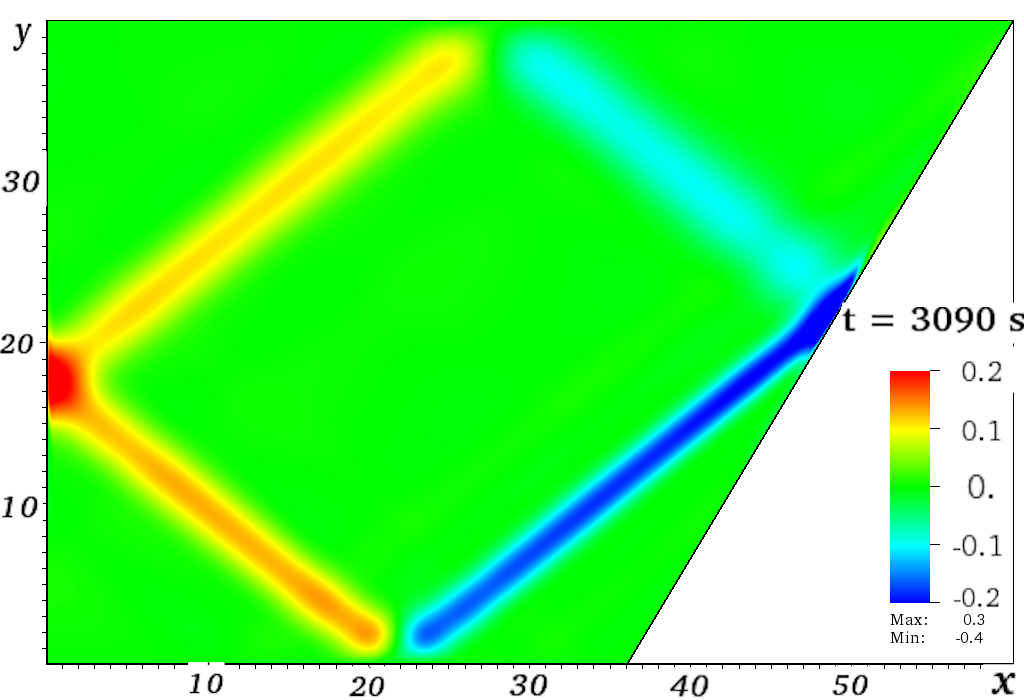
\includegraphics[scale=0.15]{pics/H40L60N1ap02dp20w0p63/2D36x36DiagramH40L60N1ap02dp20w0p63Vyn06179.png}
        \caption{Горизонтальная компонента скорости}
    \end{subfigure}
    \begin{subfigure}[с]{0.45\textwidth}
        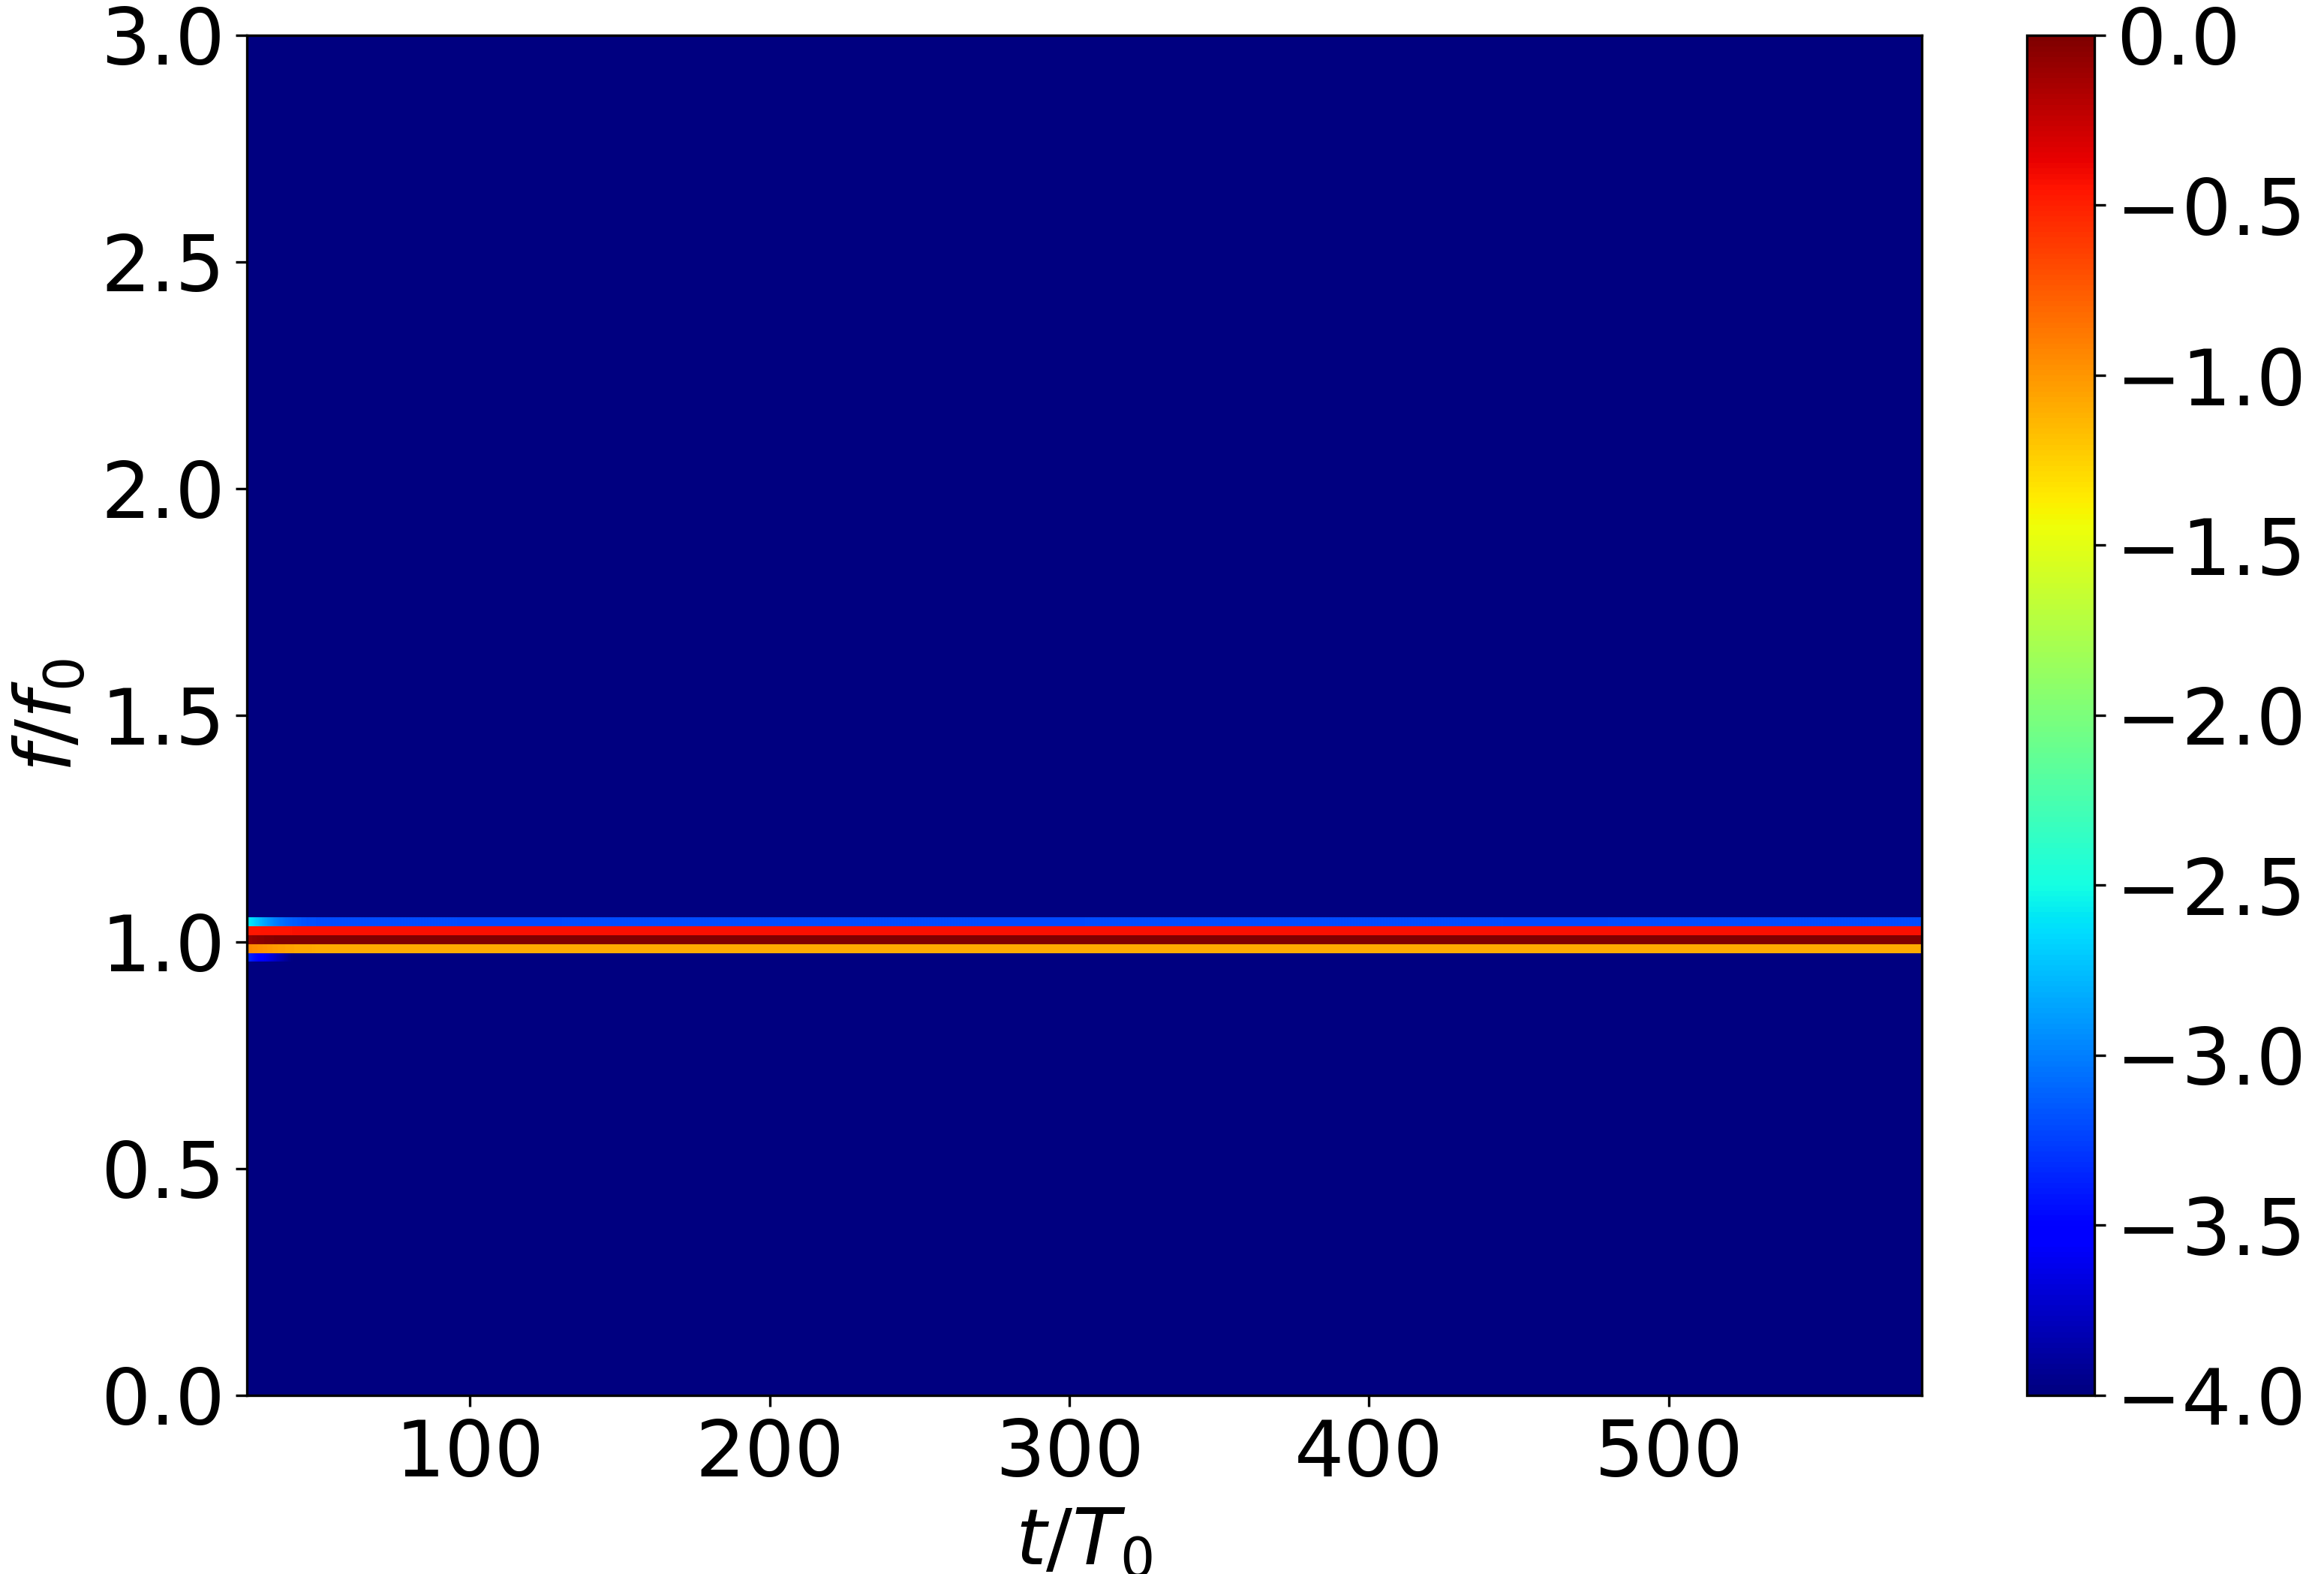
\includegraphics[scale=0.07]{pics/H40L60N1ap02dp20w0p63/TFspectrumX356Y112N1024.png}
        \caption{Частотно-временная диаграмма на аттракторе}
    \end{subfigure}
    \begin{subfigure}[с]{0.45\textwidth}
        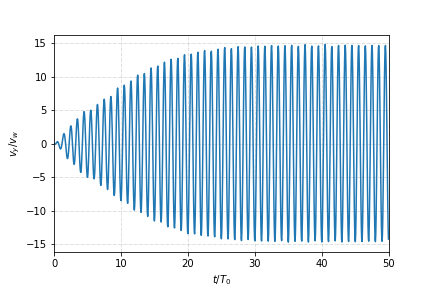
\includegraphics[scale=0.5]{pics/H40L60N1ap02dp20w0p63/vyX355662118341Y112748618745t1000.png}
        \caption{Амплитуда скорости в зависимости от времени на аттракторе}
    \end{subfigure}
    \begin{subfigure}[с]{0.45\textwidth}
        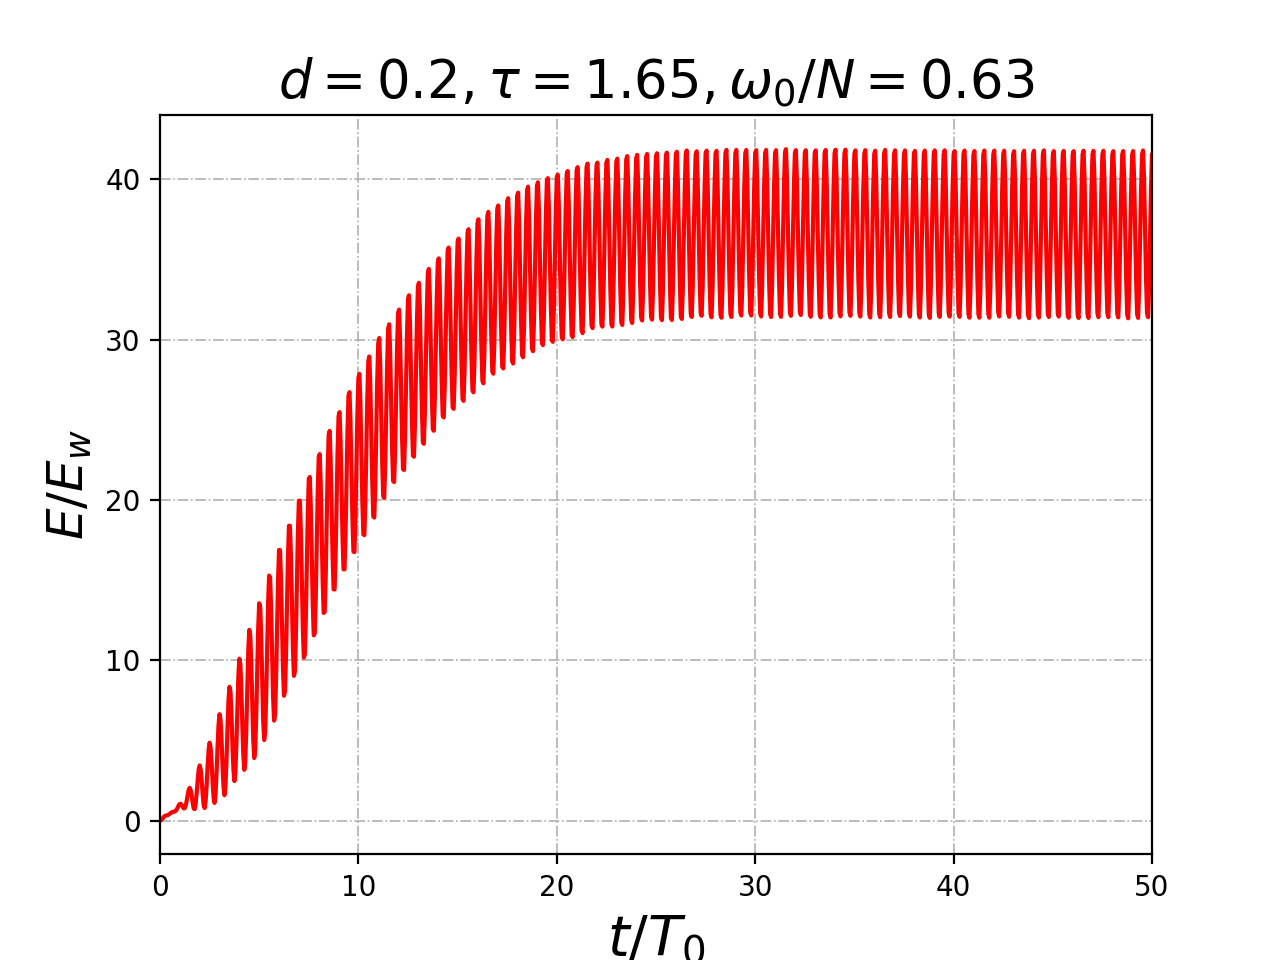
\includegraphics[scale=0.4]{pics/H40L60N1ap02dp20w0p63/2D36x36DiagramH40L60N1ap02dp20w0p63totKEnonDim.png}
        \caption{Средняя кинетическая энергия в резервуаре}
    \end{subfigure}
    
    \caption{Результат моделирования аттрактора внутренних волн методом спектральных элементов}

\end{figure}

В заключении можно сказать, что алгоритм высокого порядка точности хорошо воспроизводит результаты натурного эксперимента. В дальнейшем они будут использоваться как эталон для сравнения с остальными методами решения. 

\section{Численное моделирование аттракторов внутренних волн с помощью метода контрольного объема}

Для моделирование методом конечного объема используется конфигурация представленная на рисунке \ref{fig:dominleft} в этом случае волнопродуктор установлен на левой стенке и колеблется по следующему правилу:

\begin{equation}
    U_x = A\cdot cos\left(\frac{\pi \cdot z}{H}\right)\cdot \omega \cdot  sin(\omega_0 t)
\end{equation}

Аналогично условия на остальных стенках:

\begin{equation}
    \vec{U} = 0
\end{equation}

Для далвения:

\begin{equation}
    \nabla p = 0
\end{equation}

Для градиента солености:

\begin{equation}
    \frac{\partial s}{\partial n} = grad(s_0)
\end{equation}

В качестве алгоритма нахождения численного решения используется PISO \cite{IssaGosmanWatkins-PISO}. Вкратце изложить алгоритм нахождения полей скорости и давления можно так:
\begin{enumerate}[1.]
    \item Устанавливаются граничные условия.
    \item Решается дискредитированное уравнение движения для вычисления промежуточных значений поля скорости.
    \item Вычисляются массовые потоки через границы ячеек.
    \item Решается уравнение для давления.
    \item Корректируются массовые потоки.
    \item Корректируется поле скорости согласно новому давлению.
    \item Обновляются граничные условия.
    \item Вернуться к третьему шагу.
    \item Перейти на следующий временной шаг и начать с первого пункта.
\end{enumerate}
Внутри шага по времени тут имеется цикл между пунктом 3 и пунктом 8. Более того возможны коррекции неортогональности ячеек сетки если зациклить этот алгоритм между пунктом 4 и 5. дискредитированное уравнение движение в матричном виде можно записать следующим образом: 

\begin{equation}
    \mathcal{M} \vec{U}^* = -\frac{\nabla p}{\rho_m} + \vec{F}
\end{equation}
где $\mathcal{M}$ -- матрица коэффициентов, $\vec{U}^*$ -- искомые промежуточные значения поля скоростей. Для получения уравнения давления эта мтарица коэффициентов расщепляется следующим образом:

\begin{equation}
    \mathcal{M} \vec{U}^* = \mathcal{A} \vec{U}^* - \mathcal{\vec{H}}
\end{equation}
где $\mathcal{\vec{H}}$ -- источниковые члены для уравнения давления. $\mathcal{A}=diag(\mathcal{M})$. Подставляем расщепленную матрицу коэффициентов в уравнение движение:
\begin{equation}
    \mathcal{A} \vec{U}^* - \mathcal{\vec{H}}= -\frac{\nabla p}{\rho_m} + \vec{F}    
\end{equation}
Умножаем обе части на $\mathcal{A}^{-1}$, выражаем $\vec U$

\begin{equation}
    \mathcal{A}^{-1} \mathcal{A} \vec{U} = \mathcal{A}^{-1} \mathcal{\vec{H}} - \mathcal{A}^{-1} \nabla p + \mathcal{A}^{-1} \vec{F} \;\;=>\;\;
    \vec{U} = \mathcal{A}^{-1} \mathcal{\vec{H}} - \mathcal{A}^{-1} \nabla p + \mathcal{A}^{-1} \vec{F}
\end{equation}
согласно уравнению неразрывности $\nabla \vec{U} = 0$, это дает нам уравнение для давления:

\begin{equation}
    \nabla \cdot (\mathcal{A}^{-1} \nabla p) = \nabla \cdot (\mathcal{A}^{-1} \mathcal{\vec{H}} + \mathcal{A}^{-1} \vec{F})
\end{equation}

Алгоритм PISO не прост в понимании и сложен из-за двух вложенных циклов внутри одного временного шага. Но очень популярен и долгое время остается одним из самых востребованных инструментов вычислительное гидродинамики.

К сожалению, результаты моделирования аттрактора внутренних волн алгоритмом PISO количественно не соответствуют результатам полученным при помощи метода спектральных элементов. 

Подведя итог можно сказать следующее, популярный алгоритм качественно воспроизводит картину течения, образующуюся при многократном отражении внутренних волн от стенок трапециевидного резервуара. Но количественно нет. Преимуществом алгоритма является способность работать с неортогональными сетками и сложной геометрией. К недостаткам можно отнести сложность и нелинейность процедуры нахождения гидродинамических полей.

\begin{figure}[!ht]
    \centering
        \begin{tikzpicture}[scale=5.34, z={(-.707,-.5)}]
          \node[anchor=south west,inner sep=0] at (0,0) {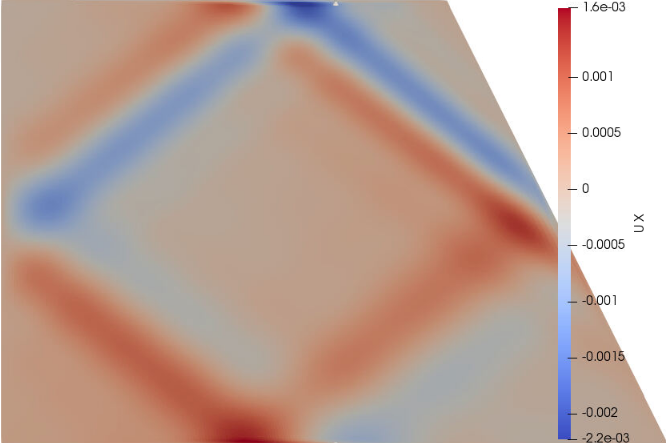
\includegraphics[width=\textwidth]{Figs/Attr200s.png}};
          \draw[thick,style = dashed] (1.5, 0, 0) -- (1.5, 2, 0);
        \end{tikzpicture}
    \caption{Поле горизонтальной компоненты скорости, пунктиром показана линия пробы}
    \label{fig:attractorRes}
\end{figure}



\begin{figure}[!ht]
    \centering
            \begin{tikzpicture}[scale = 1.1]
            \begin{axis}
                [scale only axis, grid=major,legend style={at={(0,1),font=\LARGE},anchor=north west}, ymin=-0.8*10^-3, ymax=1.7*10^-3,legend style={nodes={scale=0.5, transform shape}}, x post scale=1.6]

                \addplot[solid,color=red,thick] table [x=Points:1, y=Result, col sep=comma] {CSV/snappy180x180nCor4NonOrth4.csv};

                \addplot[solid,color=blue,thick] table [x=Points:1, y=Result, col sep=comma] {CSV/FVMnocor.csv};

                \addplot[solid,color=orange,thick,dashed] table [x=Points:1, y=Result, col sep=comma] {CSV/FVM450x2.csv};

                \legend{PISO 225x150*, PISO 225x150, PISO 450x300}
            \end{axis}
            \begin{axis}
                [scale only axis, ymin=-0.8*10^-1, ymax=1.7*10^-1, yticklabels={,,},xticklabels={,,},legend style={at={(0,0.76),font=\LARGE},anchor=north west},legend style={nodes={scale=0.5, transform shape}},x post scale=1.6]
%                \addplot[solid,thick] table [x=Points:1, y=x_velocity, col sep=comma] {CSV/Ux30Nek500T200.csv};
                \legend{NEK5000}
            \end{axis}
        \end{tikzpicture} 
    \caption{Результат моделирования с помощью агоритма PISO}
    \label{fig:PISOattr}
\end{figure}

\section{Численное моделирование аттракторов внутренних волн с помощью метода контрольного объема на базе квазигидродинамического подхода}

В этом разделе будут подробно разобраны способы аппроксимации слагаемых в квазигидродинамических уравнениях. Рассматриваются способы дискретизации уравнений и их реализация при помощи пакета с открытым исходным кодом OpenFOAM версии 1912\cite{OpenFOAM}.

OpenFOAM -- математический пакет с открытым исходным кодом. Аббревиатура FOAM означает Field Operation And Manipulation, то есть операции и манипуляции с полями. В OpenFAOM реализованные гибкие и современные инструменты как численного моделирования, так и разработки согласно современным стандартам языка С++ и объектно-ориентированного программирования. 

Для начала рассмотрим дискретные аналоги квазигидродинамических уравнений. Производные по времени аппроксимируются разностями согласно схеме Эейлера:

\begin{equation}
    \frac{\partial \vec{U}}{\partial t} \approx \frac{ \vec{U}_n-\vec{U}_o}{\Delta t}, \,\,\,
    \frac{\partial \Tilde{s}}{\partial t} \approx \frac{ \Tilde{s}_n-\Tilde{s}_o}{\Delta t},
\end{equation}
или с помощью схемы Адамса-Башфорта:

\begin{equation}
    \frac{\partial \vec{U}}{\partial t} \approx   \frac{1}{\Delta t} \left  (\frac{3}{2}\vec{U}_n - 2\vec{U}_o + \frac{1}{2} \vec{U}_{oo} \right), \,\,\,
    \frac{\partial \Tilde{s}}{\partial t} \approx \frac{1}{\Delta t} \left (\frac{3}{2}\Tilde{s}_n - 2\Tilde{s}_o + \frac{1}{2} \Tilde{s}_{oo}\right).
\end{equation}

Пространственная аппроксимация имеет второй порядок точности. Конечно-объемное представление:

\begin{equation}
        \nabla \cdot \frac{\tau}{\rho}\nabla \Tilde{p} \approx  \frac{1}{V} \sum_f \vec{S}_f \cdot \left(   \frac{\tau}{\rho} \cdot \frac{1}{V} \sum_f \vec{S}_f \cdot p  \right) ,
\end{equation}
Индекс $f$ обозначает принадлежность к поверхности.
Дискретный аналог уравнения Пуассона:

\begin{equation}
        \frac{1}{V} \sum_f \vec{S}_f \cdot \left(   \frac{\tau}{\rho} \cdot \frac{1}{V} \sum_f \vec{S}_f \cdot p  \right) = \frac{1}{V} \sum_f \left( \vec{U}_o - \tau \cdot (\vec{U}_o \cdot \nabla \vec{U}_o ) + \tau \cdot \vec{F}_o \right) \cdot \vec{S}_f,
        \label{eq:Poisson}
\end{equation}
где $o$ обозначает значение с предыдущего шага по времени.
Дискретный аналог уравнения движения:   

\begin{multline}
    \frac{ \vec{U}_n-\vec{U}_o}{\Delta t} + \frac{1}{V} \sum_f \vec{S}_f \cdot \left( \vec{U}_o \otimes \vec{U}_o - \vec{W}_o \otimes \vec{U}_o \right) \cdot \vec{S}_f - \frac{\nu}{V} \sum_f \frac{\delta\vec{U}_o}{\delta \vec{n}}\cdot |\vec{S}_f| - \\
    - \frac{1}{V} \sum_f \vec{S}_f \cdot \left( \vec{U}_o \otimes \vec{W}_o \right) \cdot \vec{S}_f = - \frac{1}{\rho} \nabla p_n + \vec{F}_o,
    \label{eq:momentumImpl}
\end{multline}
или оно может быть записано в явной форме:

\begin{multline}
    \frac{ \vec{U}_o-\vec{U}_n}{\Delta t} + \frac{1}{V} \sum_f \vec{S}_f \cdot \left( \vec{U}_o \otimes \vec{U}_o - \vec{W}_o \otimes \vec{U}_o \right) \cdot \vec{S}_f - \frac{\nu}{V} \sum_f \frac{\delta\vec{U}_n}{\delta \vec{n}}\cdot |\vec{S}_f| - \\
    - \frac{1}{V} \sum_f \vec{S}_f \cdot \left( \vec{U}_o \otimes \vec{W}_o \right) \cdot \vec{S}_f = - \frac{1}{\rho} \nabla p_n + \vec{F}_o.
    \label{eq:momentumExp}
\end{multline}

Дискретный аналог уравнения солености:

\begin{multline}
    \frac{ s_n-s_o}{\Delta t} = \frac{1}{V}\sum_f \vec{S}_f \cdot \left (\vec{U}_n - \vec{W}_n \right) \cdot s_o \cdot \vec{S}_f - \frac{\nu}{Sc \, V} \sum_f \frac{\delta s_o}{\delta \vec{n}}\cdot |\vec{S}_f| -\\
    - \frac{1}{V} \sum_f \left( \tau \vec{U}_f \cdot \vec{S}_f \cdot (\vec{U}_f \cdot \sum_f \nabla s \cdot \vec{S}_f)\right) \cdot \vec{S}_f,    
    \label{eq:salImp}
\end{multline}
или его явная версия:
\begin{multline}
    \frac{ s_n-s_o}{\Delta t} = \frac{1}{V}\sum_f \vec{S}_f \cdot \left (\vec{U}_n - \vec{W}_n \right) \cdot s_o \cdot \vec{S}_f - \frac{\nu}{Sc \, V} \sum_f \frac{\delta s_n}{\delta \vec{n}}\cdot |\vec{S}_f| -\\
    - \frac{1}{V} \sum_f \left( \tau \vec{U}_f \cdot \vec{S}_f \cdot (\vec{U}_f \cdot \sum_f \nabla s \cdot \vec{S}_f)\right) \cdot \vec{S}_f.  
    \label{eq:salExp}
\end{multline}

Аппроксимация регуляризационных членов:

\begin{itemize}
    \item Reduced, вычисляются только нормальный составляющие производных:
    \begin{equation}
        (\nabla U)_f \approx \vec{n}_f \otimes \frac{\vec{U}_{P}-\vec{U}_{S}}{|\vec{d}|} \,\,\,\,\,
        (\nabla s)_f \approx \vec{n}_f \otimes \frac{\vec{s}_{P}-\vec{s}_{S}}{|\vec{d}|},
    \end{equation}
    где $\vec{d}$ -- это длинна вектора между центрами $P$ и $N$ двух соседних ячеек. На смежной поверхности вычисляются производные.
    
    \item Метод наименьших квадратов согласно\cite{Kraposhin2017}% define as
    %\begin{equation}
        %(\nabla U)_f \approx \sum_i w_i^2 \hat{G}^{-1} \cdot \left ( \vec{d}_i \otimes %(\vec{U}_i-\vec{U}_f) \right ),
    %\end{equation}
    %where $\hat{G}$ is a tensor $\hat{G}=\sum_i w_i^2 \vec{d}_i \otimes \vec{d}_i $ and %weight $w_i=1/|\vec{d}_i|$.
    \item Метод Гаусса-Остроградского, вычисление производных осуществляется по методу Шильникова\cite{Istomina2019}. схема вычислений представлена на рисунке  \ref{fig:derOnFace}. Выражения для производных имеют простой вид для скалярных полей, для векторных и тензорных эта процедура производится покомпонентно:
    
    \begin{equation}
        \frac{\partial \alpha}{\partial x} = \frac{1}{V_f} \sum_{m=1}^8 n_{m,x} \alpha_m,
    \end{equation}
    где $m$ количество ребер, $\alpha$ дифференцируемое значения, $\alpha_m$ усредненное значение по ребру $\alpha$.
\end{itemize}

Для того чтобы найти решение квазигидродинамической системы необходимо проинтегрировать уравнение Пуассона для давления (\ref{eq:Poisson}) и вычислить новое значение этой величины. Затем нужно найти дополнительную скорость $\vec{W}$. Потом проинтегрировать уравнение движения в явной(\ref{eq:momentumExp}) или неявной (\ref{eq:momentumImpl}) форме чтобы найти поле скорости на новом временном шаге. И наконец, вычислить соленость проинтегрировав (\ref{eq:salImp}) или (\ref{eq:salExp}).
    
    %http://www.mathnet.ru/php/archive.phtml?wshow=paperjrnid=ipmppaperid= 2724optionlang=rus
    %https://getbox.ispras.ru/index.php/s/hJvMgLQo9r6xKEZ 
    
    


    \begin{figure}[!ht]
        \centering
          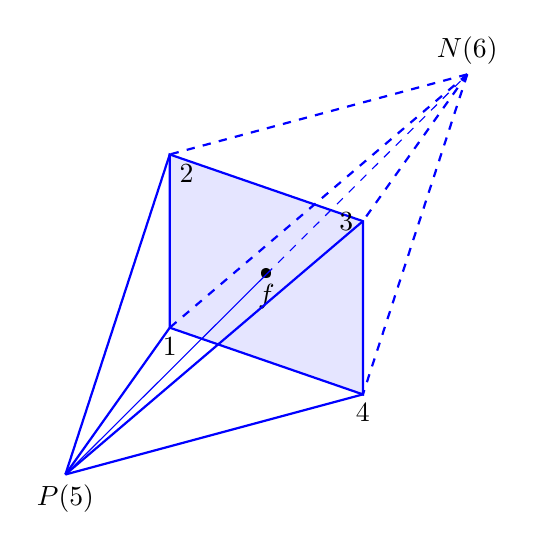
\begin{tikzpicture}[scale=1.1, every node/.style={scale=1}]
          
          ` %FACE DRAW
            \filldraw[color=blue,fill opacity=0.1,thick] (1.5,0,1)--(-1.5,0,-1)--(-1.5,2,-1)--(1.5,2,1)--cycle;
            %\draw[style=dashed,color=blue] (1.5,0,1)--(-1.5,2,-1);
            %\draw[style=dashed,color=blue] (1.5,2,1)--(-1.5,0,-1);
            \node at (0,1,0) {\textbullet};
            \draw (0,1,0) node[below] {$f$};
            
            \draw  (1.5,0,1) node[below] {$4$};
            \draw  (-1.5,0,-1) node[below] {$1$};
            \draw  (-1.5,2,-1) node[below right] {$2$};
            \draw  (1.5,2,1) node[left] {$3$};

            \draw [color=blue] (0,1,0)--(-0.01,1,6);
            \draw [color=blue,dashed] (0,1,0)--(0.01,1,-6);
            \draw  (-0.01,1,6) node[below] {$P(5)$};
            \draw  (0.01,1,-6) node[above] {$N(6)$};
            
            \draw [color=blue,thick] (-0.01,1,6)--(1.5,0,1);
            \draw [color=blue,thick] (-0.01,1,6)--(-1.5,0,-1);
            \draw [color=blue,thick] (-0.01,1,6)--(-1.5,2,-1);
            \draw [color=blue,thick] (-0.01,1,6)--(1.5,2,1);
            
            \draw [color=blue,thick,dashed] (0.01,1,-6)--(1.5,0,1);
            \draw [color=blue,thick,dashed] (0.01,1,-6)--(-1.5,0,-1);
            \draw [color=blue,thick,dashed] (0.01,1,-6)--(-1.5,2,-1);
            \draw [color=blue,thick,dashed] (0.01,1,-6)--(1.5,2,1);
            
          \end{tikzpicture}
        \caption{Схема вычисления производных на поверхности $f$, $P$ центр текущей ячейки, $N$ центр соседней ячейки.}
        \label{fig:derOnFace}
    \end{figure}


Преимущество квазигидродинамических уравнений в том, что алгоритм их решения линейный без вложенных циклов внутри одного временного шага. Уравнение для давления находится сразу без громоздких процедур, которые необходимо проделать в PISO. Графическое описание можно увидеть на рисунке \ref{fig:blockScheme}. Алгоритм поиска решения заключается в следующем:

\begin{figure}[!h]

    \tikzstyle{decision} = [diamond, draw, 
    text width=4.5em, text badly centered, node distance=3cm, inner sep=0pt]
    \tikzstyle{block} = [rectangle, draw, 
    text width=30em, text centered, minimum height=3em, minimum width=30em]
    \tikzstyle{line} = [draw, -latex']
    \tikzstyle{cloud} = [draw, ellipse,fill=red!20, node distance=3cm,
    minimum height=2em]
    \centering
    \begin{tikzpicture}[node distance = 2cm, auto]
    % Place nodes
        \node [block] (UpdateF) {Обнавляются поля (1)};
        \node [block, below of=UpdateF] (UpdateFl) {Обновляются потоки (2)};
        \node [block, below of=UpdateFl] (Control) {Считываются параметры рассчета (3)};
        \node [block, below of=Control] (Stability) {Вычисление параметров устойчивости (4)\\ $|\vec{U}_c|\cdot \frac{\Delta t}{\Delta x}$ and $\Delta t < \tau \cdot C$};
%       
        \node [block, below of=Stability] (Increasing) {Увеличение временного шага (5) \\ $t^n = t^o + \Delta t$ };
        \node [block, below of=Increasing] (Store) {Сохраняются поля с предыдущего временного шага (6)};
        \node [block, below of=Store] (Adjustment) {Поправка скорости обуслеовленная турбулентностью (7)};
        \node [block, below of=Adjustment] (Pressure) {Явное вычисление поля давления (8)};
        \node [block, below of=Pressure] (Velocity) {Явное или неявное вычисление поля скоростей (9)};
        \node [block, below of=Velocity] (Salinity) {Явное или не явное вычисление поля солености (10)};

        \path [line] (UpdateF) -- (UpdateFl);
        \path [line] (UpdateFl) -- (Control);
        \path [line] (Control) -- (Stability);
        \path [line] (Stability) -- (Increasing);
        \path [line] (Increasing) -- (Store);
        \path [line] (Store) -- (Adjustment);
        \path [line] (Adjustment) -- (Pressure);
        \path [line] (Pressure) -- (Velocity);
        \path [line] (Velocity) -- (Salinity);
    \end{tikzpicture}
    
    \caption{Алгоритм QHDFoam}
    \label{fig:blockScheme}
\end{figure}

\begin{enumerate}[1)]
  \item Обновляются поля на поверхностях для давления, солености, скорости и массовой силы на новом временном слое путем интерполяции. Также вычисляются градиенты скоростей и солености с помощью процедуры поиска производных на поверхностях(fvsc).
  \item Обнавляются потоки через границы ячеек.
  \item Считываются параметры контроля за расчетом.
  \item Вычисляются условия устойчивости $|\vec{U}_c|\cdot \frac{\Delta t}{\Delta x}$ и $\Delta t < \tau \cdot C$
  \item Увеличивается шаг по времени $t^n = t^o + \Delta t$.
  \item Сохраняются значения полей из предыдущих временных слоев.
  \item Изменение поле скорости согласно модели турбулентности. 
  \item Явное вычисление поле давления.
  \item Явное или неявное вычисление поля скоростей.
  \item Явное или неявное вычисление поля солености.
\end{enumerate}

fvsc процедура вычисления производных на поверхностях была реализована отдельно. Для этого в OpenFOAM было разработано специальное пространство имен с интерфейсом для конкретного кейса с задачей. Пользователь может выбрать одну из схем приведенных выше используя соответствующие ключевые слова. Также небходимо выбрать способ вычисления регуляризационного параметра $\tau$. Предполагается что перед тем, как подстраивать этот параметр он будет выбран сообразно некоторым характерным безразмерным числам для конкретной задачи. Параметр настраивается для каждой задачи отдельно.

Реализация неявного вычисления уравнения движения в терминах OpenFOAM представлен на рисунке \ref{fig:velList}.

\lstset{style=mystyle}

\begin{figure}[!ht]
\centering
\begin{lstlisting}
    gradPf = fvsc::grad(p);
    Wf = tauQGDf*((Uf & gradUf) + gradPf/rhof - BdFrcf);
    surfaceVectorField phiUfWf = mesh.Sf() & (Uf * Wf);
    phiUf -= phiUfWf;

    {
    solve
        (
            fvm::ddt(U)
            +
            fvc::div(phiUf)
            -
            fvm::laplacian(muf/rhof,U)
            -
            fvc::div(muf/rhof * mesh.Sf() 
            & qgdInterpolate(Foam::T(fvc::grad(U))))
            ==
            -
            fvc::grad(p)/rho
            +
            BdFrc
            +
            USu
        );
    }
\end{lstlisting}
\caption{Исходный код вычисления уравнения движения}
\label{fig:velList}
\end{figure}

\verb gradPf   это градиент на грани который вычисляется согласно схемам, описанным выше. В файле \verb fvSchemes   можно найти пользовательский интерфейс для нее (см. Рис.  \ref{fig:fvscList})

\begin{figure}[!h]
    \centering
    
\begin{lstlisting}

    fvsc
    {
        default    GaussVolPoint;
    }

\end{lstlisting}

    \caption{Пользовательский интерфейс для fvsc}
    \label{fig:fvscList}
\end{figure}

Пользовательский интерфейс для настойки параметра регуляризации, опорные значения для давления и переключатели для явных/неявных вычислений содержится в файле \verb thermophysicalProperties   пример представлен на рис. \ref{fig:QGD}


\begin{figure}[!h]
    \centering
\begin{lstlisting}

    QGD
    {
        pRefCell        0;
        pRefValue       0;
        implicitDiffusion true;
        QGDCoeffs constTau;
        constTauDict
        {
            Tau 0.005;
        }
    }

\end{lstlisting}    
    \caption{ Пользовательский интерфейс для настройки параметра регуляризации, опорного значения для давления, а также переключатель для явного или неявного решения диффузионных слагаемых.}
    \label{fig:QGD}
\end{figure}

\subsection{Верификация}



QHDSolver это программа для моделирования движения несжимаемой жидкости. Важным свойством таких программ является чувствительность к физическим параметрам, таким как скорость, плотность, вязкость и размеры расчетной области. Эти параметры объеденяются в число рейнольдса. Также необходимо найти корректное решения для уравнения переноса. QHDSolver позиционируется как программа призванная работать с неортогональными сетками и находить корректное решение. Для демонстрации возможности решателя было выбрано несколько типовых задач. Для верификации возможности работы с неортогональными сетками была выбрана задача скошенной каверны. Чувствительность к числу Рейнольдса проверяется на задаче обратного уступа. Корректность решения уравнения переноса проверяется на задаче естественной конвекции. Полученные результаты сравниваются с результатами других исследователей.

\paragraph{Скошенная каверна}

Квазигидродинамический решатель сравнивается с PISO алгоритмом на метках низкого качества. Главной целью этого сравнения является демонстрация возможностей программы корректно решать задачи поставленные на неортогональных сетках и сложных геометриях. Эксперимент определяется следующими настроечными параметрами:

\begin{itemize}
    \item Размер сетки
    \item Шаг по времени
    \item Параметр регуляризации
    \item Число Рейнольдса
    \item Угол скошенности($\alpha$)
\end{itemize}

Моделирование исследует сеточную сходимость при числах рейнольдса 100 и 1000, углах скошенности $\alpha = \{45^{\circ}, 30^{\circ}, 15^{\circ}$\}. Схематично рассчетная область изображена на рисунке \ref{fig:skewedCavityScratch}. На верхней границе задана постоянная скорость $\vec{U}_b$ и нулевой градиент для давления. На других стенках установлено условие нулевой скорости и градиента давления.

\begin{figure}[!h]
    \centering
    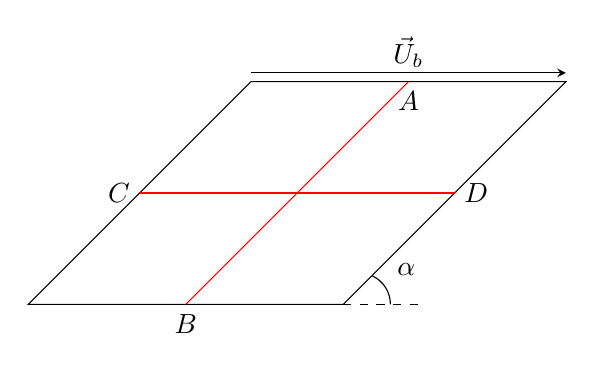
\begin{tikzpicture}[scale=4, every node/.style={scale=1}]
            \draw (0,0,0)--(1,0,0)--(1.7071,0.7071,0.0)--(0.7071,0.7071,0.0)--cycle;
            \draw [color=red] (0.5,0,0)--(1.2071,0.7071,0);
            \draw [color=red] (0.3535,0.3535,0)--(1.3535,0.3535,0);
            
            \draw [->,>=stealth](0.7071,0.735,0.0)-- (1.7071,0.735,0.0);
            \draw  (1.2071,0.72,0) node[above] {$\vec{U}_b$};
            
            \draw  (0.5,0,0) node[below] {$B$};
            \draw  (1.2071,0.7071,0) node[below] {$A$};
            \draw  (0.3535,0.3535,0) node[left] {$C$};
            \draw  (1.3535,0.3535,0) node[right] {$D$};
            
            \draw [dashed] (1,0,0)--(1.25,0,0);
            
            \draw (1.15,0) arc (0:65:1mm);
            
            \draw (1.2,0.06,0) node[above] {$\alpha$};
            
    \end{tikzpicture}
    \caption{Skewed cavity scratch}
    \label{fig:skewedCavityScratch}
\end{figure}

Компоненты поля скорости, полученные с помощью QHDFoam сравниваются с теми же компонентами полученными при помощи pimpleFOAM. Рассматревается зависимость решения от параметра регуляризации и шага по времени. Результаты моделирования также сравниваются с результатами полученными ранее другими исследователями \cite{Hines2008,Erturk2007}. 

Сравнение QHD и PIMPLE алгоритмом с числами рейнольдса $Re=100$ и $Re=1000$ $\alpha = 45^{\circ}$, $\alpha = 30^{\circ}$ демонстрируют схожесть результатов (см рис. \ref{fig:Re10045UxVSy} - \ref{fig:15UxVSYRe100}). Сетки с элементами более чем 20х20 дают отличное соотвествие с эталонным решением \cite{Erturk2007}. Для случаев с маленькими углами скошенности и числами Рейнольдса алгоритмы типа PISO не могут найти решение без коррекций на неортогональность. QHDFoam могут быть применены без дополнительных коррекций, для этого требуется увеличить параметр регуляризации или уменьшить шаг по времени.

Каждая конфигурация каверны исследована на сеточную сходимость. Обычно сетки более 40х40 элементов дают точность с ошибкой не более 5\%. Более подробные сетки дают точность с ошибкой меньше чем 3\%. Результаты сеточной сходимости приведены на рисунке \ref{fig:meshconv}, он показывает порядок метода между теоретическими линиями соответствующих первому и второму порядку.

Разность результатов полученных при помощи квазигидродинамического подхода и при помощи PISO представленная на рисунках \ref{fig:15UxVSYRe100} -- \ref{fig:r15} может быть объяснена дополнительной диссипацией, которая привносится квазигидродинамическим алгоритмом. Очевидно, что ошибка тем меньше чем, меньше параметр регуляризации. Начальное значение для этого параметра может быть выбрано согласно значению числа Рейнольдса и условию устойчивости:

\begin{equation}
    \Delta t \leq c \cdot \tau,
\end{equation}

Где $\Delta t$ это шаг по времени, $\tau$ это регуляризационный параметр, коэффициент $c$ зависит от скошенности. Опытным путем установлено что для $\alpha = 90^{\circ}$ $c=2$, но для $\alpha = 15^{\circ}$ $c=24$.

Для увеличения точности PISO алгоритма на неортогональных сетках требуется увеличивать сеточное разрешения и количество коррекций на неортогональность. Для увеличения точности квазигидродинамического алгоритма кроме увеличения количества ячеек необходимо уменьшить шаг по времени и параметр регуляризации согласно условию устойчивости(см. рис. \ref{fig:tauconv}). 

\begin{figure}[!ht]
    \centering
        \begin{tikzpicture}[scale = 1.2]
        
            \begin{axis}
                [scale only axis, grid=major, ymin=0, ymax=0.75, xmax = 1, xmin = -0.2, legend style={at={(1,0.71)},anchor=north east},legend style={nodes={scale=1, transform shape}},xlabel={$y$}, ylabel={$U_x$}]
                \addplot[solid,thick, color=red] table [y=Points:1, x=U:0, col sep=comma]     {PISOVSQHD/PISOUxVSY100Re20.csv};
                \addplot[solid,thick, color=orange] table [y=Points:1, x=U:0, col sep=comma]     {PISOVSQHD/PISOUxVSY100Re40.csv};

                \addplot[solid,thick, color=green] table [y=Points:1, x=U:0, col sep=comma]     {PISOVSQHD/QHDUxVSY100Re20.csv};
                \addplot[solid,thick, color=cyan] table [y=Points:1, x=U:0, col sep=comma]     {PISOVSQHD/QHDUxVSY100Re40.csv};
                \addplot[solid,thick, color=blue] table [y=Points:1, x=U:0, col sep=comma]     {PISOVSQHD/QHDUxVSY100Re80.csv};
                \addplot[solid,thick, color=black] table [y=Y, x=Ux, col sep=comma]     {PISOVSQHD/Eth45Re100.csv};
                \legend{PISO 20x20, PISO 40x40, QHD 20x20, QHD 40x40, QHD 80x80, Eth}
            \end{axis}
        
        \end{tikzpicture}
        \caption{Re=100, $\alpha = 45^\circ$, зависимость $U_x$ от $y$, скорость вдоль линии AB.}
        \label{fig:Re10045UxVSy}
\end{figure}

\begin{figure}[!ht]
    \centering
        \begin{tikzpicture}[scale = 1.2]
        
            \begin{axis}
                [scale only axis, grid=major, ymin=0, ymax=0.525, xmax = 1, xmin = -0.2, legend style={at={(1,0.5)},anchor=north east},legend style={nodes={scale=0.8, transform shape}},xlabel={$U_x$}, ylabel={$y$}]
                \addplot[solid,thick, color=red] table [y=Points:1, x=U:0, col sep=comma]     {PISOVSQHD/PISO30UxVSY1000Re20.csv};
                \addplot[solid,thick, color=orange] table [y=Points:1, x=U:0, col sep=comma]     {PISOVSQHD/PISO30UxVSY1000Re40.csv};
                \addplot[solid,thick, color=yellow] table [y=y, x=U_0, col sep=comma]     {PISOVSQHD/PISOCor30UxVSY1000Re80.csv};
                \addplot[solid,thick, color=green] table [y=Points:1, x=U:0, col sep=comma]     {PISOVSQHD/QHD30UxVSY1000Re20.csv};
                \addplot[solid,thick, color=cyan] table [y=Points:1, x=U:0, col sep=comma]     {PISOVSQHD/QHD30UxVSY1000Re40.csv};
                \addplot[solid,thick, color=blue] table [y=Points:1, x=U:0, col sep=comma]     {PISOVSQHD/QHD30UxVSY1000Re80.csv};
                \addplot[only marks, color=black] table [y=Y, x=Ux, col sep=comma]     {PISOVSQHD/Eth30UxVSYRe1000.csv};
                \legend{PISO 20x20, PISO 40x40,  PISO 80x80*, QHD 20x20, QHD 40x40, QHD 80x80, Eth}
            \end{axis}
        
        \end{tikzpicture}
        \caption{Re=1000, $\alpha = 30^\circ$, зависимость $U_x$ от $y$, горизонтальная компонента сокрости вдоль линии AB.}
        \label{fig:30UxVSY1000Re}
\end{figure}


\begin{figure}[!ht]
    \centering
        \begin{tikzpicture}[scale = 1]
            \begin{axis}[scale only axis, grid=major, ymin=-2.2*10^-2, ymax=2*10^-2, xmin = 0.42, xmax = 1.45, legend style={at={(0.4,1)},anchor=north east},legend style={nodes={scale=0.8, transform shape}},xlabel={$x$}, ylabel={$U_y$}]

                \addplot[solid,thick, color=red] table [x=Points:0, y=U:1, col sep=comma]     {PISOVSQHD/PISO30UyVSX1000Re20.csv};
                \addplot[solid,thick, color=orange] table [x=Points:0, y=U:1, col sep=comma]     {PISOVSQHD/PISO30UyVSX1000Re40.csv};
                \addplot[solid,thick, color=yellow] table [x=x, y=U_1, col sep=comma]     {PISOVSQHD/PISOCor30UyVSX1000Re80.csv};
                \addplot[solid,thick, color=green] table [x=Points:0, y=U:1, col sep=comma]     {PISOVSQHD/QHD30UyVSX1000Re20.csv};
                \addplot[solid,thick, color=cyan] table [x=Points:0, y=U:1, col sep=comma]     {PISOVSQHD/QHD30UyVSX1000Re40.csv};
                \addplot[solid,thick, color=blue] table [x=Points:0, y=U:1, col sep=comma]     {PISOVSQHD/QHD30UyVSX1000Re80.csv};
                \addplot[only marks, color=black] table [x=X, y=Uy, col sep=comma]     {PISOVSQHD/Eth30UyVSXRe1000.csv};
                \legend{PISO 20x20, PISO 40x40, PISO 80x80*, QHD 20x20, QHD 40x40, QHD 80x80, Eth}
            \end{axis}
         \end{tikzpicture}
         \caption{Re=1000, $\alpha = 30^\circ$, зависимость $U_y$ от $x$, вертикальная компонента скорости вдоль линии CD, звездочкой обозначен результат проведенный с помощью коррекций на неортогональность}
         \label{fig:30UyVSXRe1000}
\end{figure}


\begin{figure}[!ht]
     \centering
         \begin{tikzpicture}[scale = 1]
             \begin{axis}
             [scale only axis, grid=major, ymin=0, ymax=0.3, xmax = 1, xmin = -0.2, legend style={at={(1,0.71)},anchor=north east},legend style={nodes={scale=1, transform shape}},xlabel={$U_x$}, ylabel={$y$}]
                 \addplot[solid,thick, color=red] table [y=Points:1, x=U:0, col sep=comma] {PISOVSQHD/PISOCor15UxVSY100Re80.csv};
                 \addplot[solid,thick, color=green] table [y=Points:1, x=U:0, col sep=comma]     {PISOVSQHD/QHD15UxVSY100Re20.csv};
                 \addplot[solid,thick, color=cyan] table [y=Points:1, x=U:0, col sep=comma]     {PISOVSQHD/QHD15UxVSY100Re40.csv};
                 \addplot[solid,thick, color=blue] table [y=y, x=U_0, col sep=comma] {PISOVSQHD/UxVSY15Re100M80Tu5.csv};
                 \addplot[only marks, color=black] table [y=Y, x=Ux, col sep=comma]     {PISOVSQHD/Eth15UxVSYRe100.csv};
                 \legend{PISO 80x80*, QHD 20x20, QHD 40x40, QHD 80x80, Eth};
             \end{axis}
         \end{tikzpicture}
         \caption{Re=100, $\alpha = 15^\circ$, зависимость $U_x$ от $y$, горизонтальная компонента скорости вдоль линии AB, звездочкой обозначены результаты полученный с использованием поправок на неортогональность}
         \label{fig:15UxVSYRe100}
\end{figure}

\begin{figure}[!ht]
    \centering
        \begin{tikzpicture}[scale = 1.2]
            \begin{axis}[scale only axis, grid=major, ymin=-8.2*10^-2, ymax=12*10^-2, xmin = 0.5, xmax = 1.5, legend style={at={(0.5,0.36)},anchor=north east},legend style={nodes={scale=0.8, transform shape}},xlabel={$x$}, ylabel={$U_y$}]
                \addplot[solid,thick, color=red] table [x=Points:0, y=U:1, col sep=comma]     {PISOVSQHD/PISOCor15UyVSX100Re80.csv};
                \addplot[solid,thick, color=green] table [x=Points:0, y=U:1, col sep=comma]     {PISOVSQHD/QHD15UyVSX100Re20.csv};
                \addplot[solid,thick, color=cyan] table [x=Points:0, y=U:1, col sep=comma]     {PISOVSQHD/QHD15UyVSX100Re40.csv};
                \addplot[solid,thick, color=blue] table [x=x, y=U_1, col sep=comma] {PISOVSQHD/UyVSX15Re100M80Tu5.csv};
                \addplot[only marks, color=black] table [y=Uy, x=x, col sep=comma]     {PISOVSQHD/Eth15UyVSXRe100.csv};
                \legend{PISO 80x80*, QHD 20x20, QHD 40x40, QHD 80x80, Eth};
            \end{axis}
        \end{tikzpicture}
        \caption{Re=100, $\alpha = 15^\circ$, зависимость $U_y$ от $x$, вертикальная компонента скорости вдоль линии AB, звездочкой обозначены результаты полученные с использованием поправок на неортогональность}
        \label{fig:15UyVSXRe100}
\end{figure}

 \begin{figure}[!ht]
     \centering
         \begin{tikzpicture}[scale = 1.2]
            \begin{axis}
                [scale only axis, grid=major, ymin=-4.8*10^-2, ymax=3*10^-2, xmin = 0.47, xmax = 1.5, legend style={at={(0.5,0.5)},anchor=north east},legend style={nodes={scale=0.6, transform shape}},xlabel={$x$}, ylabel={$U_y$}]
                \addplot[solid,thick, color=red] table [x=Points:0, y=U:1, col sep=comma]     {PISOVSQHD/QHD15UyVSX1000Re512.csv};
                \addplot[only marks, color=black] table [x=X, y=Uy, col sep=comma]     {PISOVSQHD/Eth15UyVSXRe1000.csv};
                \addplot[solid,thick, color=blue] table [x=Points:0, y=U:1, col sep=comma]     {PISOVSQHD/QHD15UyVSX1000Re80Tu24.csv};
                \addplot[solid,thick, color=cyan] table [x=Points:0, y=U:1, col sep=comma]     {PISOVSQHD/QHD15UyVSX1000Re80Tu10.csv};
                 \addplot[solid,thick, color=gray] table [x=Points:0, y=U:1, col sep=comma]     {PISOVSQHD/QHD15UyVSX1000Re80Tu5.csv};
                \legend{QHD 512x512, Eth, QHD 80x80 $\tau = 0.024$, QHD 80x80 $\tau = 0.010$, QHD 80x80 $\tau = 0.005$};
            \end{axis}
         \end{tikzpicture}
         \caption{Re=1000, $\alpha = 15^\circ$, зависимость $U_y$ от $x$, влияние параметра регуляризации на решение.}
         \label{fig:r15}
 \end{figure}

\begin{figure}[!ht]
    \centering
        \begin{tikzpicture}[scale = 1.2]
            \begin{axis}
                [scale only axis, grid=major, ymin=-4.8*10^-2, ymax=3*10^-2, xmin = 0.47, xmax = 1.5, legend style={at={(0.6,0.5)},anchor=north east},legend style={nodes={scale=0.8, transform shape}},xlabel={$x$}, ylabel={$U_y$}]
                \addplot[solid,thick, color=red] table [x=Points:0, y=U:1, col sep=comma]     {PISOVSQHD/QHD15UyVSX1000Re512.csv};
                \addplot[only marks, color=black] table [x=X, y=Uy, col sep=comma]     {PISOVSQHD/Eth15UyVSXRe1000.csv};
                \addplot[solid,thick, color=blue] table [x=Points:0, y=U:1, col sep=comma]     {PISOVSQHD/QHD15UyVSX1000Re80Tu24.csv};
                \addplot[solid,thick, color=cyan] table [x=Points:0, y=U:1, col sep=comma]     {PISOVSQHD/QHD15UyVSX1000Re80Tu10.csv};
                 \addplot[solid,thick, color=gray] table [x=Points:0, y=U:1, col sep=comma]     {PISOVSQHD/QHD15UyVSX1000Re80Tu5.csv};
                \legend{QHD 512x512, Eth, QHD 80x80 $\tau = 0.024$, QHD 80x80 $\tau = 0.010$, QHD 80x80 $\tau = 0.005$};
            \end{axis}
        \end{tikzpicture}
        \caption{Re=1000, $\alpha = 15^\circ$, зависимость $U_y$ от $x$}
        \label{fig:tauconv}
\end{figure}

\begin{figure}[!ht]
    \centering
        \begin{tikzpicture}[scale = 1.5]
            \begin{axis}
                [ymode=log,xmode=log,xlabel={Number of cells}, ylabel={$L_1 error$}]
                \addplot[solid,thick, color=red] table [x=N, y=L1, col sep=comma]{PISOVSQHD/meshConv.csv};
                \addplot[solid,thick,dashed, color=blue] table [x=N, y=L1, col sep=comma]
                {PISOVSQHD/meshConvEth.csv};
                \addplot[solid,thick,dashed, color=green] table [x=N, y=L1, col sep=comma]{PISOVSQHD/meshConvEth1Ord.csv};
            \end{axis}
        \end{tikzpicture}
        \caption{Сеточная сходимость, порядок метода}
        \label{fig:meshconv}
\end{figure}

\begin{figure}
    \centering
        \begin{tikzpicture}[scale = 1.2]
            \begin{axis}
                [scale only axis, grid=major, ymin=-0.02, ymax=0.25, xmin = 0.0, xmax = 1.1, legend style={at={(0.45,0.9)},anchor=north east},legend style={nodes={scale=1, transform shape}}]
                \addplot[solid,thick, color=black] table [x=l, y=UyTau0.004, col sep=comma]     {CSV/AllTau.csv};
                \addplot[solid,thick, color=orange] table [x=l, y=UyTau0.005, col sep=comma]     {CSV/AllTau.csv};
                \addplot[solid,thick, color=green] table [x=l, y=UyTau0.01, col sep=comma]     {CSV/AllTau.csv};
                \addplot[solid,thick, color=cyan] table [x=l, y=UyTau0.02, col sep=comma]     {CSV/AllTau.csv};
                \addplot[solid,thick, color=gray] table [x=l, y=UyTau0.04, col sep=comma]     {CSV/AllTau.csv};
                \addplot[solid,thick, color=brown] table [x=l, y=UyTau0.08, col sep=comma]     {CSV/AllTau.csv};
                \addplot[solid,thick, color=red] table [x=l, y=UyTau0.16, col sep=comma]     {CSV/AllTau.csv};
                \legend{$\tau = 0.004$, $\tau = 0.005$, $\tau = 0.01$, $\tau = 0.02$, $\tau = 0.04$,$\tau = 0.08$,$\tau = 0.16$}
            \end{axis}
        \end{tikzpicture}
        \caption{Re=1000, $\alpha = 45^\circ$, $U_y$ vs $x$, влияние параметра регуляризации на решение}
\end{figure}



\paragraph{Обратный уступ}

Для моделирования вязкой жидкости, алгоритму необходимо быть чувствительным к изменению числа Рейнольдса. Задача обратного уступа это простой и эффективный способ проверить эту чувствительность. На вход в расчетную область подается параболический профиль скорости. Все стенки кроме входа и выхода подчиняются условию прилипания для скорости и нулевого градиента для давления. 

После стабилизации потока измеряется расстояния от левой твердой стенки до точки разворота потока($d$) (см рис. \ref{fig:backwardStepScratch}). Полученное значение $d$ сравнивается с эталонным из \cite{ElizarBook}. Результаты показывают что QHDFoam корректно разрешает вязкие течения (см. рис. \ref{StreamRe100})

\begin{figure}[!h]
    \centering
    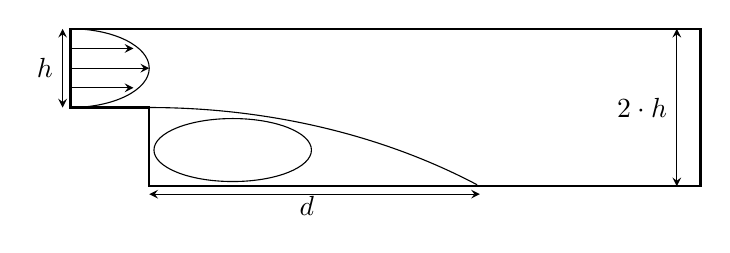
\begin{tikzpicture}[scale=1, every node/.style={scale=1}]
        \draw[thick] (0,2,0)--(0,1,0)--(1.0,1.0,0.0)--(1.0,0.0,0.0)--(8.0,0.0,0.0)--(8.0,2.0,0.0)--cycle;
            
        \draw (0.0,1.0) arc(-90:90:1cm and 0.5cm);
        \draw [->,>=stealth](0.0,1.5,0.0)-- (1,1.5,0.0);
        \draw [->,>=stealth](0.0,1.25,0.0)-- (0.8,1.25,0.0);
        \draw [->,>=stealth](0.0,1.75,0.0)-- (0.8,1.75,0.0);
        
        
        \draw (2.06,0.06) arc(-90:270:1cm and 0.4cm);
        \draw [<->,>=stealth](1,-0.1)--(5.2,-0.1);
        \draw (3,0.0,0) node[below] {$d$};
        
        \draw [<->,>=stealth](-0.1,1)--(-0.1,2);
        \draw (-0.1,1.5,0) node[left] {$h$};
        
        \draw [<->,>=stealth](7.7,0)--(7.7,2);
        \draw (7.7,1,0) node[left] {$2 \cdot h$};
        \draw (1.0,1.0) arc(90:53.5:7cm and 5cm);
    \end{tikzpicture}
    \caption{Схематичное изображение задачи с обратным уступом.}
    \label{fig:backwardStepSketch}
\end{figure}

\begin{figure}[!h]
    \centering
    \begin{subfigure}{\textwidth}
        \centering
        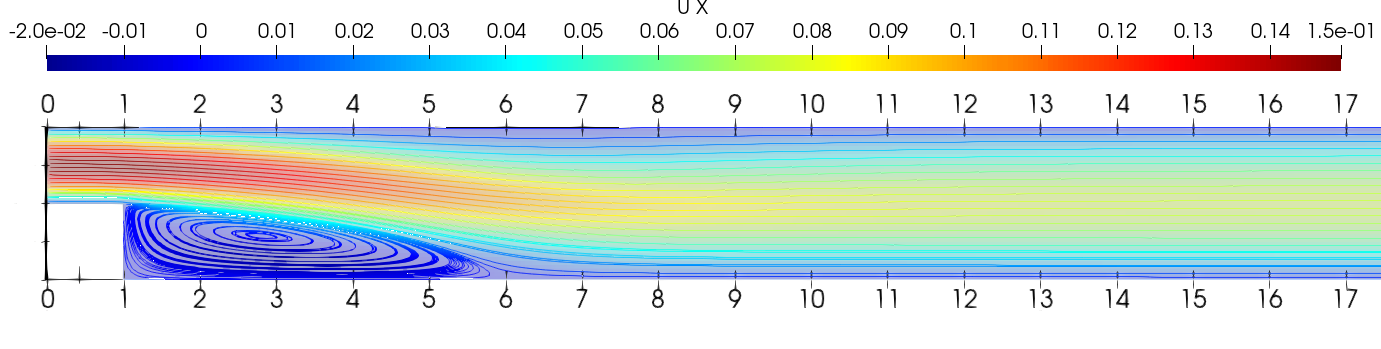
\includegraphics[scale=0.4]{pics/Re100.png}
        \caption{Re=100}
    \end{subfigure}
    \begin{subfigure}{\textwidth}
        \centering
        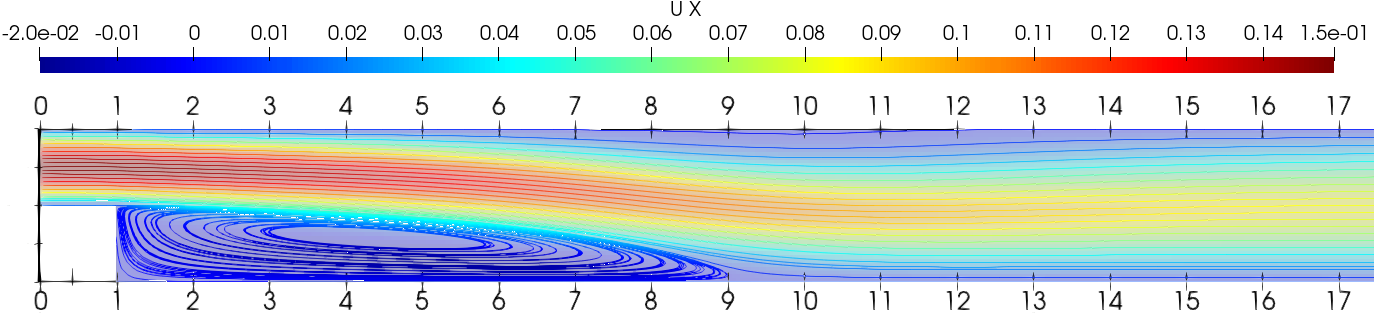
\includegraphics[scale=0.4]{pics/Re200.png}
        \caption{Re=200}
    \end{subfigure}
    \begin{subfigure}{\textwidth}
        \centering
        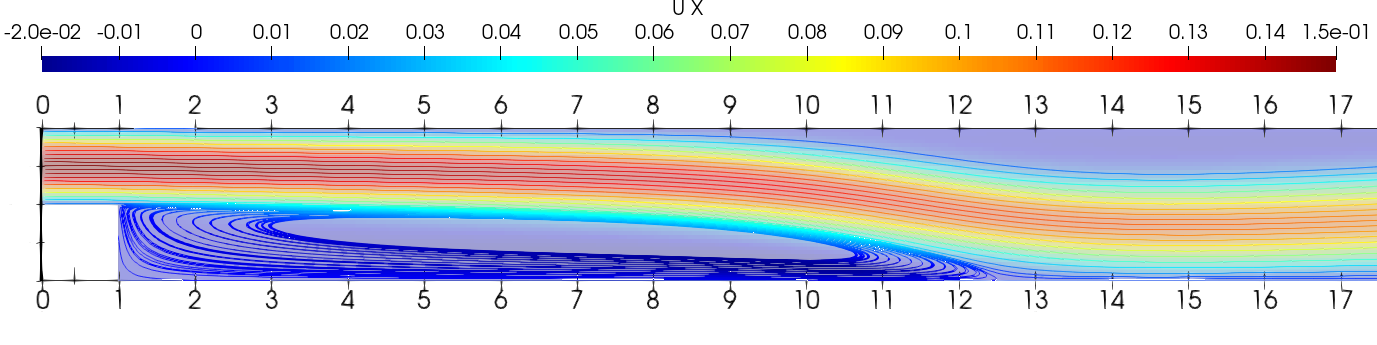
\includegraphics[scale=0.4]{pics/Re400.png}
        \caption{Re=400}
    \end{subfigure}
    \caption{Линии тока для задачи с обратным уступом}
    \label{StreamRe100}
\end{figure}


\begin{table}[!hb]
\caption {Сравнение результатов для задачи обратного уступа}
\noindent\begin{tabular}{l|ccc}
Research & $Re=100$ & $Re=200$  & $Re=400$ \\
\hline
QHDFoam & 5.0 & 8.25 & 11.9\\
Sparrow E. M. and Chuck W.\cite{Sparrow1987} & 5.0 & 7.5 & -\\
Kim J. and Moin P.\cite{Kim1985} & 5.0 & 8.3 & 12 \\
Hackman L. P. et al.\cite{Hackman1984} & 5.0 & 8.5 & -\\
\hline
Armaly B. F. et al.\cite{Armaly1983} & 5.0 & 8.5 & 14.2
\end{tabular}
\label{table:tabBackward}
\end{table}

\paragraph{Естественная конвекция}

Рассматривается задача естественной конвекции в каверне согласно \cite{ElizarBook} значение регуляризационного параметра было вычислено пропорционально обратному числу Грастгофа $Gr^{-1}$, которое было порядка $10^{-4}$ с. Сравнение максимумов горизонтальной и вертикальной скорости с данными из \cite{ElizarBook} и \cite{Vabishevich} показывают сеточную сходимость и хорошую согласованность между QHDFoam и рассматриваемыми в работах методами. Результаты сравнения видны в таблице \ref{table:tabHotCavityHor} . Линии тока изображены на рисунке \ref{fig:Nconv}. Схему расчетной области можно увидеть на рисунке \ref{fig:convectionScratch}

\begin{table}[!hb]
\caption { Сравнение максимума горизонтальной компоненты скорости для задачи естественной конвекции.}
\noindent\begin{tabular}{l|ccc}
Mesh & $U_x$ \cite{ElizarBook} & $U_x$ \cite{Vabishevich} & $U_x$ \textit{QHDFoam} \\
\hline
$20\times20$ & 15.938 & 16.144 & 16.040\\
$40\times40$ & 16.005 & 16.262 & 16.410\\
$80\times80$ & 16.070 & 16.219 & 16.225
\end{tabular}
\label{table:tabHotCavityHor}
\end{table}

 \begin{table}[!h]
\centering
\caption {Сравнение максимума вертикальной компоненты скорости для задачи естественной конвекции.}
\noindent\begin{tabular}{l|ccc}
Mesh & $U_y$ \cite{ElizarBook} & $U_y$ \cite{Vabishevich} & $U_y$ \textit{mulesQHDFoam} \\
\hline
$20\times20$ & 19.513 & 19.363 & 19.670\\
$40\times40$ & 19.663 & 19.602 & 19.910\\
$80\times80$ & 19.663 & 19.648 & 19.757
\end{tabular}
\label{table:tabHotCavityVer}
\end{table}

\begin{figure}
    \centering
    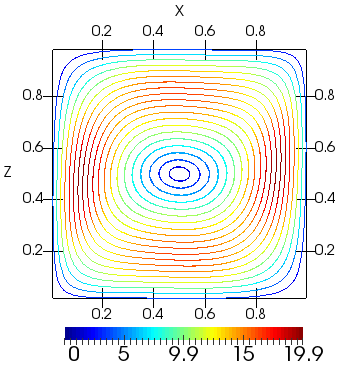
\includegraphics[scale=0.9]{pics/Umag.png}
    \caption{Линии тока для задачи естественной конвекции}
    \label{fig:Nconv}
\end{figure}

\begin{figure}
    \centering
    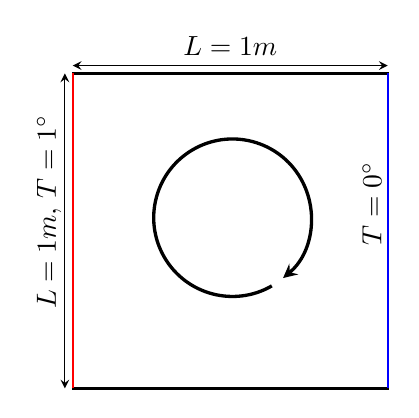
\begin{tikzpicture}[scale = 4]
        \draw[thick] (0,0,0) -- (1,0,0) -- (1,1,0) -- (0,1,0) -- cycle;
        
        \draw[thick, color = red] (0,0,0) -- (0,1,0);
        
        \draw[thick, color = blue] (1,0,0) -- (1,1,0);
        \draw (0.95,0.75) node[left,rotate=90] {$T=0^{\circ}$};
        
        \draw [<->,>=stealth](-0.025,0)--(-0.025,1);
        \draw (-0.075,0.9) node[left,rotate=90] {$L=1 m,$  $T=1^{\circ}$};
        
        \draw [<->,>=stealth](0,1.025)--(1,1.025);
        \draw (0.5,1.025) node[above] {$L=1 m$};
        \draw[ very thick,->, >=stealth] (0.15,0.9)  ++ (-50:.75) arc (300:-50:.25 and .25);
        
    \end{tikzpicture}
    \caption{Схематичное изображение задачи для естественной конвекции}
    \label{fig:convectionScratch}
\end{figure}

\subsection{Валидация}


Аттрактор внутренних волн -- это сложное явление, которое происходит после многократного отражения внутренних волн от стенок резервуара. PISO алгоритмы из предыдущего раздела не справляются с моделированием этого феномена, но результаты моделирования аттрактора с помощью решателя QHDFoam показывают неплохие результаты. Удалось добиться ошибки меньше 3\% см. Рис. \ref{fig:AdamsBashforthEulerNek3D}.

\begin{figure}[hbt!]
    \centering
        
    \begin{tikzpicture}[scale = 1,spy using outlines={circle, magnification=6, connect spies}]
        \begin{axis}
            [scale only axis, xlabel=Линия пробы $m \cdot 10^{-3}$, ylabel=$U_x\;\; m/s \cdot 10^{-3}$, grid=major,legend style={at={(0,1),font=\LARGE},anchor=north west}, ymin=-0.8, ymax=0.8,xmin=0,xmax=20,legend style={nodes={scale=0.5, transform shape}}, x post scale=1.6]

            \addplot[solid,color=black,thick] table [x=Points:1, y=U, col sep=comma] {CSV/NEK5000.csv};
            \addplot[solid,color=red,thick] table [x=Points:1, y=U, col sep=comma] {CSV/QHD480x320.csv};
            \addplot[solid,color=green!60!black,thick] table [x=Points:1, y=U, col sep=comma] {CSV/QHD240x160.csv};
            \addplot[solid,color=blue,thick] table [x=Points:1, y=U, col sep=comma] {CSV/QHD240x1602tau.csv};
            \legend{NEK500,QHDFoam 480x320, QHDFoam 240x160, QHDFoam 240x160 $\tau \cdot 2$}

            \coordinate (spypoint) at (axis cs:14.7,0.7);
            \coordinate (magnifyglass) at (axis cs:15.5,-0.3);
        \end{axis}
        \spy [blue, size=4cm] on (spypoint) in node[fill=white] at (magnifyglass);
    \end{tikzpicture} 
    \caption{Количественное сравнение результатов моделирования}
    \label{fig:AdamsBashforthEulerNek3D}
\end{figure}


Также количественные исследования демонстрируют сходимость решения получаемое с помощью квазигидродинамических уравнений к решению полученному с помощью метода высокого порядка (см. Рис. \ref{fig:tauAttr}) в отличии от результатов полученных с помощью PISO (см. Рис. \ref{fig:PISOattr}).

\begin{figure}
    \centering
        \begin{tikzpicture}[scale = 1.1]
          \begin{axis}
             [scale only axis, grid=major,legend style={at={(0,1),font=\LARGE},anchor=north west}, ymin=-0.8*10^-3, ymax=1.7*10^-3, xmin=0.0,legend style={nodes={scale=0.5, transform shape}}, x post scale=1.5,xlabel={$y$}, ylabel={$U_x$}];
            \addplot[solid,color=red,thick] table [x=Points:1, y=U:0, col sep=comma] {CSV/Ux300.5tau.csv};
            \addplot[solid,color=green,thick] table [x=Points:1, y=-U:0, col sep=comma] {CSV/Ux301tau.csv};
            \addplot[solid,color=blue,thick] table [x=Points:1, y=U:0, col sep=comma] {CSV/Ux302tau.csv};
            %\addplot[solid,color=violet,dashed,thick] table [x=Points:1, y=-U:0, col sep=comma] {CSV/Ux30tau001200sBackward.csv};
            \legend{$\tau = 0.005$,$\tau = 0.01$,$\tau = 0.02$,Adams-Bashforth}
          \end{axis}
          \begin{axis}
            [scale only axis, ymin=-0.8*10^-1, ymax=1.7*10^-1, xmin=0.0,  yticklabels={,,},xticklabels={,,},legend style={at={(0,0.75),font=\LARGE},anchor=north west},legend style={nodes={scale=0.5, transform shape}},x post scale=1.5];
            \addplot[solid,thick] table [x=Points:1, y=x_velocity, col sep=comma] {CSV/Ux30Nek500T200.csv};
            \legend{NEK5000}
          \end{axis}
        \end{tikzpicture} 
    \caption{Распределение скорости вдоль линии AB. Демонстрируется сходимость по $\tau$.}
    \label{fig:tauAttr}
\end{figure}


\section{Критические частоты и диапазон существования аттракторов внутренних волн}

Для фокусировки внутренних гравитационных волн используется стратифицированная жидкость с линейным профилем стратификации и трапециевидный резервуар, который может, служит линзой для внутренних гравитационных вол и фокусировать их в аттракторы внутренних гравитационных вол. При этом эффект фокусировки зависит от угла распространения внутренних волн и геометрических параметров резервуара. Аттрактор образуется далеко не при каждой комбинации этих параметров. Возможные геометрии резервуаров подробно описаны в работе Лео Мааса\cite{Maas1995}. Также там описывается процедура перехода к универсальным координатам $(d,\tau)$ это резко сокращает количество определяющих задачу параметров. Предполагается, что параметры резервуара являются фиксированными, а варьируется лишь частота колебания волнопродуктора причем этого достаточно чтобы управлять формой аттрактора. В данном разделе осуществляется поиск универсальных частот волнопродуктора, которые бы обеспечивали образование аттрактора внутренних гравитационных волн. 

Для поиска использовалась диаграмма из работы Лео Мааса\cite{Maas1997}. Найдем такие параметры системы, чтобы аттрактор вырождался в отрезки для этого положим $\tau=2$. Выбор такого значения обусловлен углом распространения внутренних волн $\theta = 45^{\circ}$. Это значит, что волна пущенная из левого верхнего угла упрется в правый нижний угол так как длинна резервуара $=2$ от $-1$ до $1$(см рис. \ref{fig:trivAttr}). Если в уравнение (\ref{eq:transformZ}) подставить вместо $z$ высоту резервуара $H$ то получим:

\begin{equation}
    \tau=\frac{2H}{L} \sqrt{\frac{N^2}{\omega^2}-1}.
\end{equation}

Теперь подставим $\tau=2$:

\begin{equation}
    1=\frac{H}{L} \sqrt{\frac{N^2}{\omega^2}-1}.
\end{equation}

Выразим отсюда $\omega$:

\begin{equation}
    \omega=\frac{NH}{\sqrt{L^2+H^2}}.
\end{equation}

\begin{figure}
    \centering
    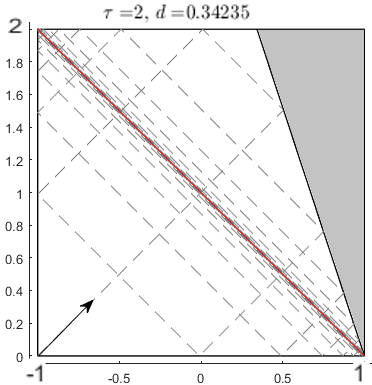
\includegraphics[scale=0.8]{Figs/CritAttrFreq.png}
    \caption{Вырожденный аттрактор внутренних волн.}
    \label{fig:trivAttr}
\end{figure}

Теперь найдем второй случай, при котором аттрактор зажимается между двумя противоположными углами. Это означает что луч пущенный из левого нижнего угла должен попасть в точку $d$. То есть $\tau = 1+d$:

\begin{equation}
    1+d=\frac{2H}{L} \sqrt{\frac{N^2}{\omega^2}-1}.
\end{equation}

Выразим отсюда частоту $\omega$:

\begin{equation}
    \omega = \frac{NH}{\sqrt{\left( 1-H\cdot tg(\alpha) \right)^2+H^2}}.
\end{equation}

После процедуры рейтрейсинга(см рис. \ref{fig:attrTriv})
    
\begin{figure}
    \centering
    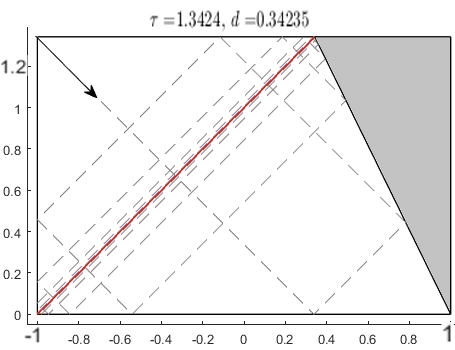
\includegraphics[scale=0.6]{Figs/AttrCritFreq.png}
    \caption{Вырожденный аттрактор внутренних волн.}
    \label{fig:attrTriv}
\end{figure}


Также с помощью метода спектральных элементов случаи вырожденных аттракторов были смоделированы(см. рис. \ref{fig:critNekfr}).

\begin{figure}
    \centering
    
    \begin{subfigure}[с]{1\textwidth}
        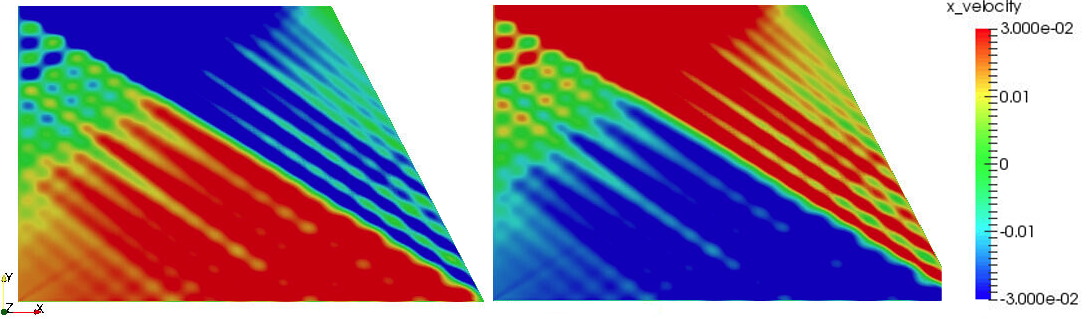
\includegraphics[scale=0.45]{Figs/AttrNEKcrit1.png}
        \caption{Расчет при помощи метода спектральных элементов с первой критической частотой}
    \end{subfigure}
    
    \begin{subfigure}[r]{1\textwidth}
        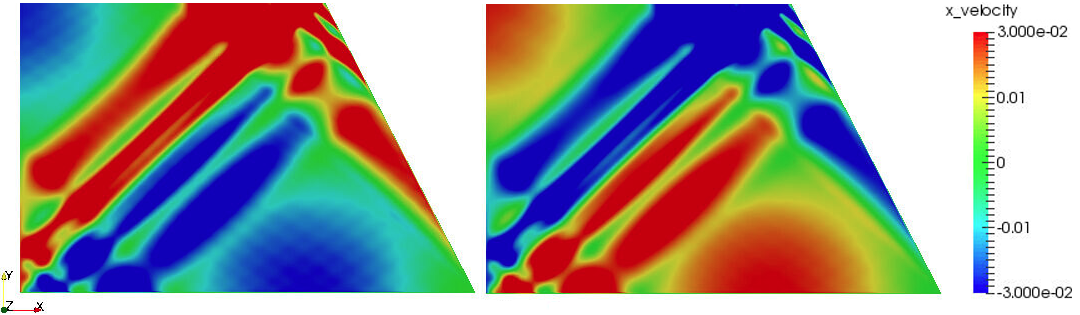
\includegraphics[scale=0.45]{Figs/AttrNekCrit2.png}
        \caption{Расчет при помощи метода спектральных элементов со второй критической частотой}
    \end{subfigure}
    \caption{Результаты расчетов при колебании волнопродуктора с критическими частотами}
    \label{fig:critNekfr}
\end{figure}

Критические значения замыкают собой диапазон частот, колебания волнопродуктора с которыми будет приводить к образованию аттрактора:

\begin{equation}
    \omega_{c_{1}}=\frac{NH}{\sqrt{L^2+H^2}}, \;\;\;\;\;\;\;\;\; \omega_{c_{2}} = \frac{NH}{\sqrt{\left( 1-H\cdot tg(\alpha) \right)^2+H^2}},
\end{equation}


\begin{equation}
    \omega_{c_{1}} \leq \omega_A \leq \omega_{c_{2}}.
\end{equation}

Этот раздел дает ответ на вопрос о том какие частоты приводят к образованию аттрактора внутренних гравитационных волн в резервуаре. Эти частоты зависят только от геометрических параметров резервуара и частоты плавучести.

\section{Волновые движения в замкнутом резервуаре при воздействии с двумя частотами}

Известно, что в океане существует великое множество волн. Вопрос будут ли волны различных частот мешать образовываться аттрактору до сих пор остается открытым. В данной работе изучается вопрос совместного воздействия на стратифицированную жидкость волнопродуктора с двумя различными частотами и одинаковой амплитудой. 

Постановка задачи несколько меняется. Для моделирования используется конфигурация представленная на рисунке \ref{fig:domainup}. Условие на волнопродукторе будет теперь записываться следующим образом:

\begin{equation}
    U_z = A_1\cdot cos\left(\frac{\pi \cdot z}{L_1}\right)\cdot \omega_1 \cdot  sin(\omega_1 t) + A_2\cdot cos\left(\frac{\pi \cdot z}{L_1}\right)\cdot \omega_2 \cdot  sin(\omega_2 t)
\end{equation}

Посчитаны различные режимы:

\begin{itemize}
    \item Режим разнесенными частотами, $\omega_1/N=0.58$ $\omega_2/N=0.66$ и малой амплитудой $a=0.02$ см. 
    \item Режим с совпадающими частотами, $\omega_1=\omega_2=0.628$ и амплитудой $a=0.05$ см.
    \item Режим с приближенными частотами, $\omega_1/N=0.66$ $\omega_2/N=0.68$ и амплитудой $a=0.05$ см.
    \item Режим с близкими частотами $\omega_1/N=0.628$ $\omega_2/N=0.641$ и  амплитудой $a=0.05$ см.
\end{itemize}

Первый режим демонстрирует общую картину течения при взаимодействии с двумя частотами. На рисунке \ref{fig:biharmVyamp02} показано, что в одном резервуаре допустимо существования сразу двух аттракторов внутренних волн. Это видно по характерному распределению поля скоростей и давлений в резервуаре. В середине первого(том что соединяет нижнюю и наклонную стенку) луче аттрактора помещена точка пробы. Видно, что существует задержка между частотой колебания волнопродуктора и частотой колебаний в середине первого луча аттрактора. Помимо этого, построен спектр частот колебаний скорости, частоты на этом графике осреднены по большей из частот. Сама точка пробы также размещена на первом луче аттрактора, который возникает под воздействием большей из частот. Это объясняет то почему второй пик меньше. На протяжении всей частотно-временной диаграммы наблюдается доминация этих двух частот.

\begin{figure}
  \centering
    \begin{subfigure}[с]{0.45\textwidth}
        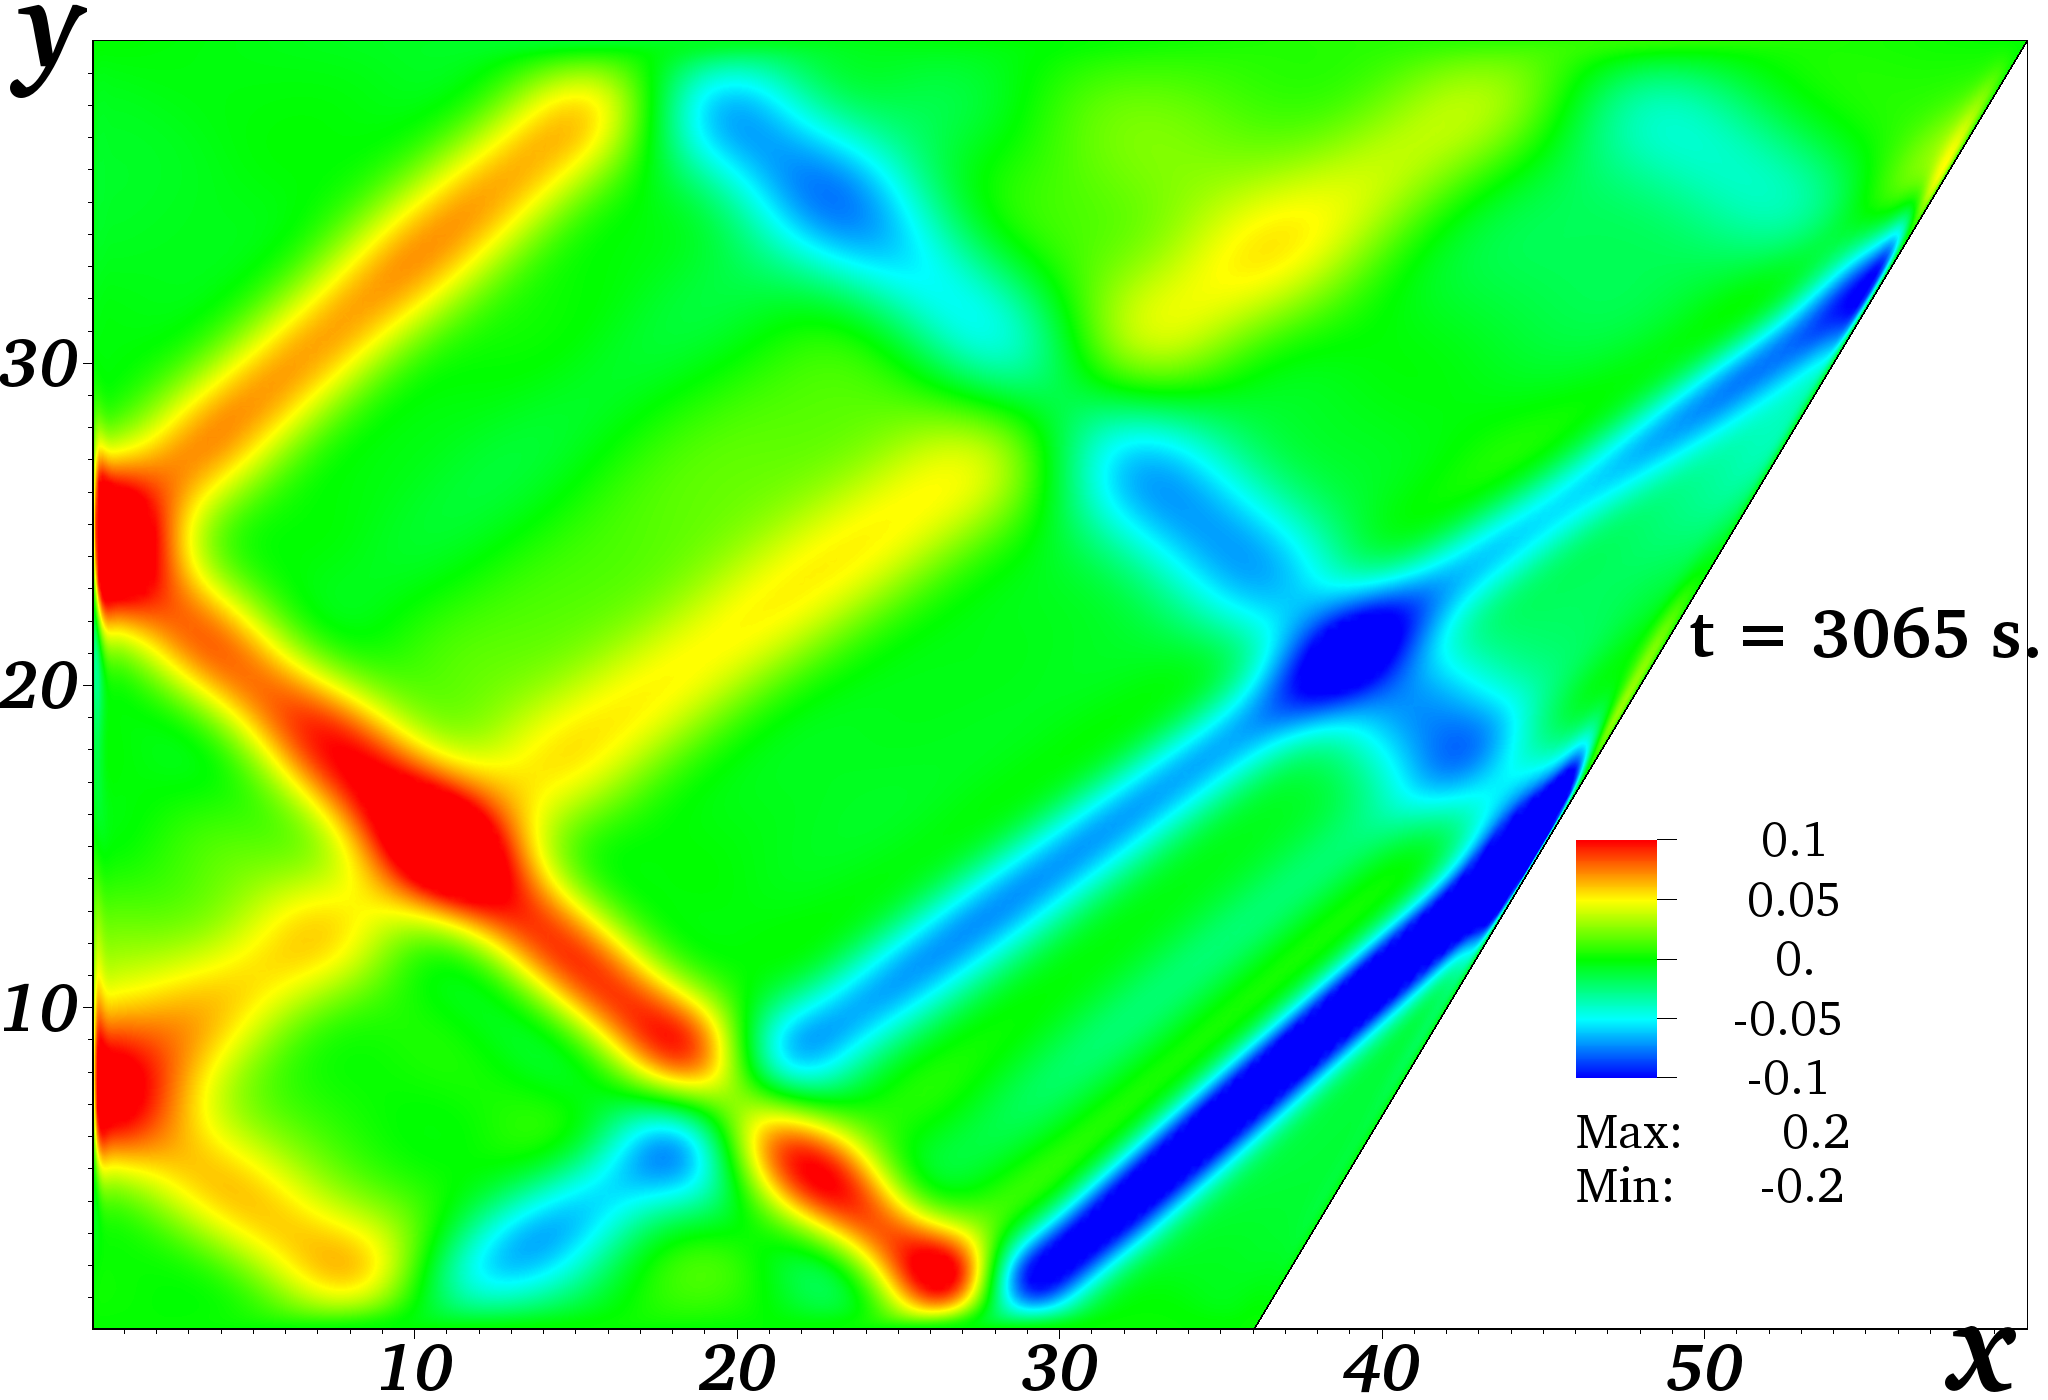
\includegraphics[width=1\textwidth]{pics/H40L60N1ap02dp20w1p58w2p66Biharm/2D36x36DiagramH40L60N1ap02dp20w1p58w2p66BiharmVyn06129.png}
        \caption{Вертикальная компонента скорости}
    \end{subfigure}
    \begin{subfigure}[с]{0.45\textwidth}
        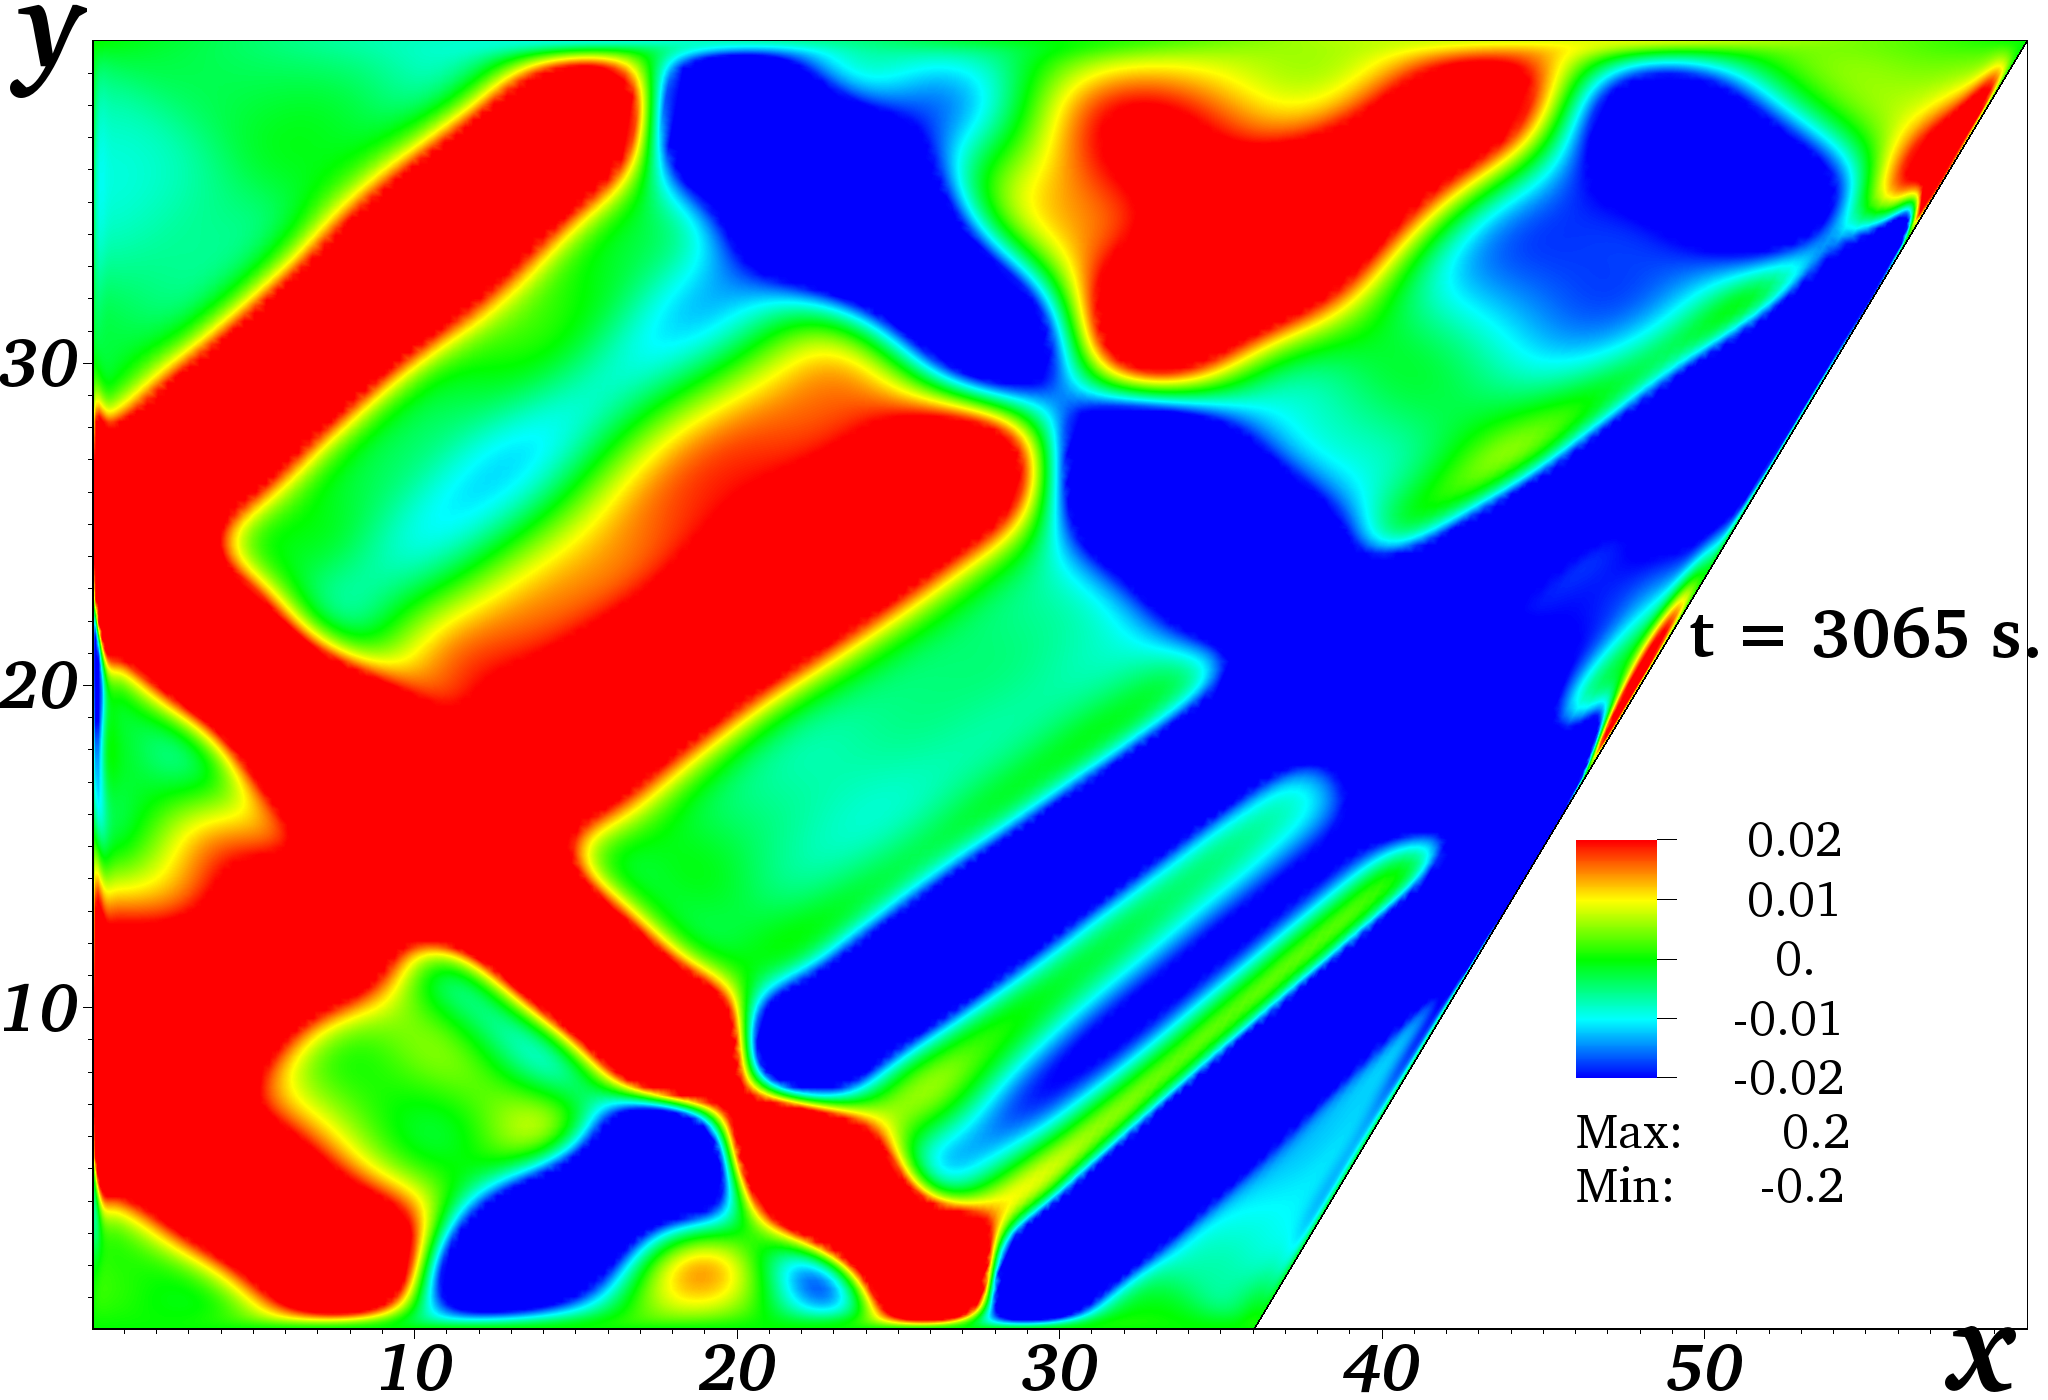
\includegraphics[width=1\textwidth]{pics/H40L60N1ap02dp20w1p58w2p66Biharm/2D36x36DiagramH40L60N1ap02dp20w1p58w2p66BiharmVy6129.png}
        \caption{Поле давления}
    \end{subfigure}
    \par
    \begin{subfigure}[с]{0.45\textwidth}
        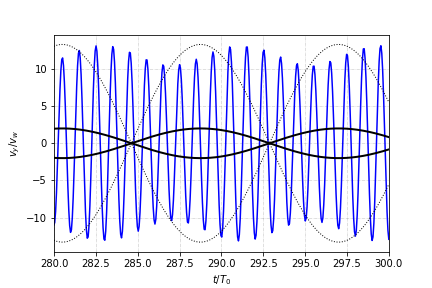
\includegraphics[width=1\textwidth]{pics/H40L60N1ap02dp20w1p58w2p66Biharm/vyX36p49Y7p94frm280to300.png}
        \caption{Вертикальная компонента скорости в середине первого луча аттрактора}
    \end{subfigure}
    \begin{subfigure}[с]{0.45\textwidth}
        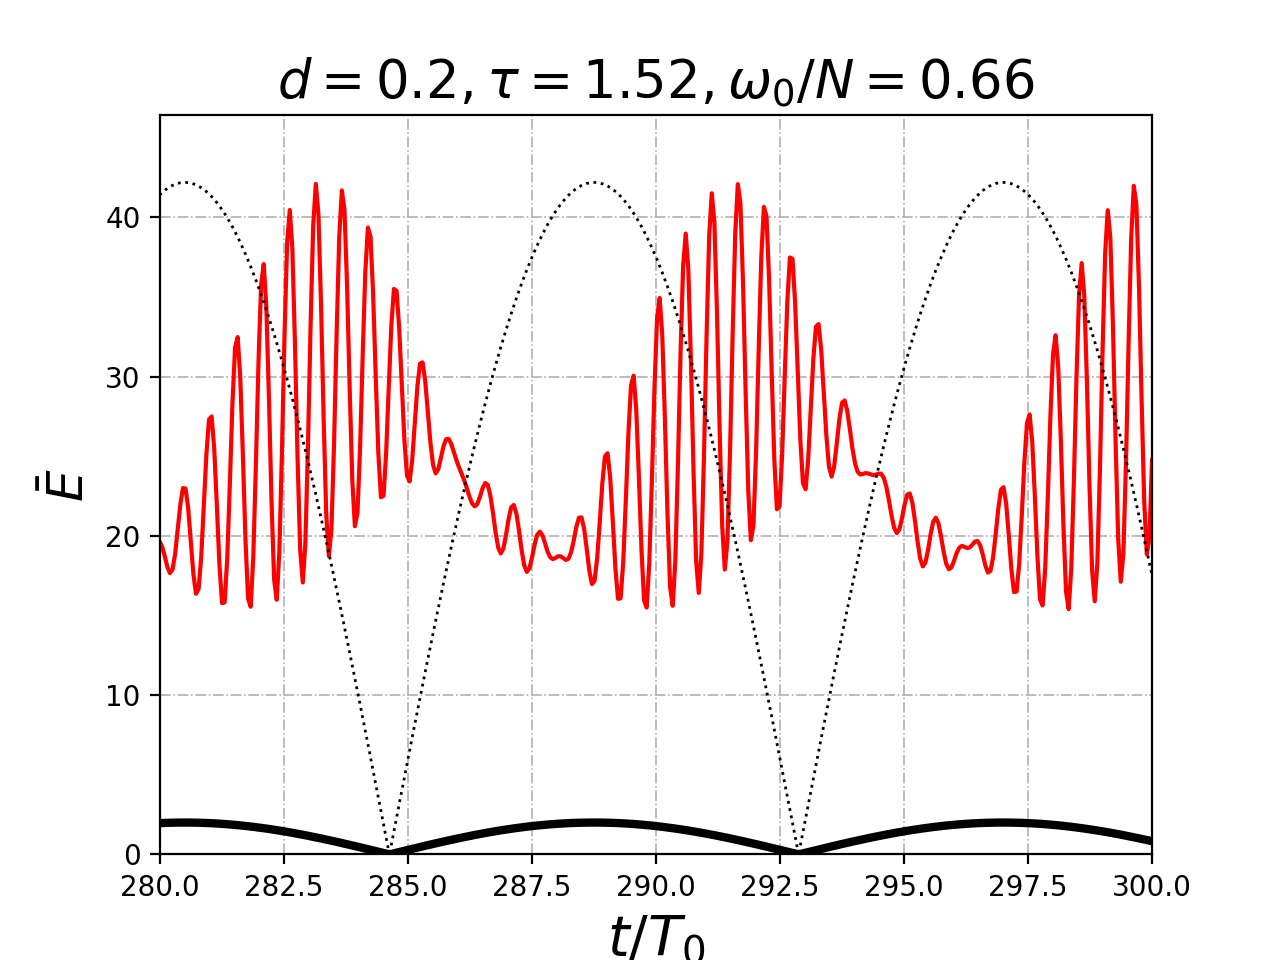
\includegraphics[width=1\textwidth]{pics/H40L60N1ap02dp20w1p58w2p66Biharm/2D36x36DiagramH40L60N1ap02dp20w1p58w2p66BiharmtotKEnonDim.png}
        \caption{Средняя кинетическая энергия в резервуаре}
    \end{subfigure}
    \par
    \begin{subfigure}[с]{0.45\textwidth}
        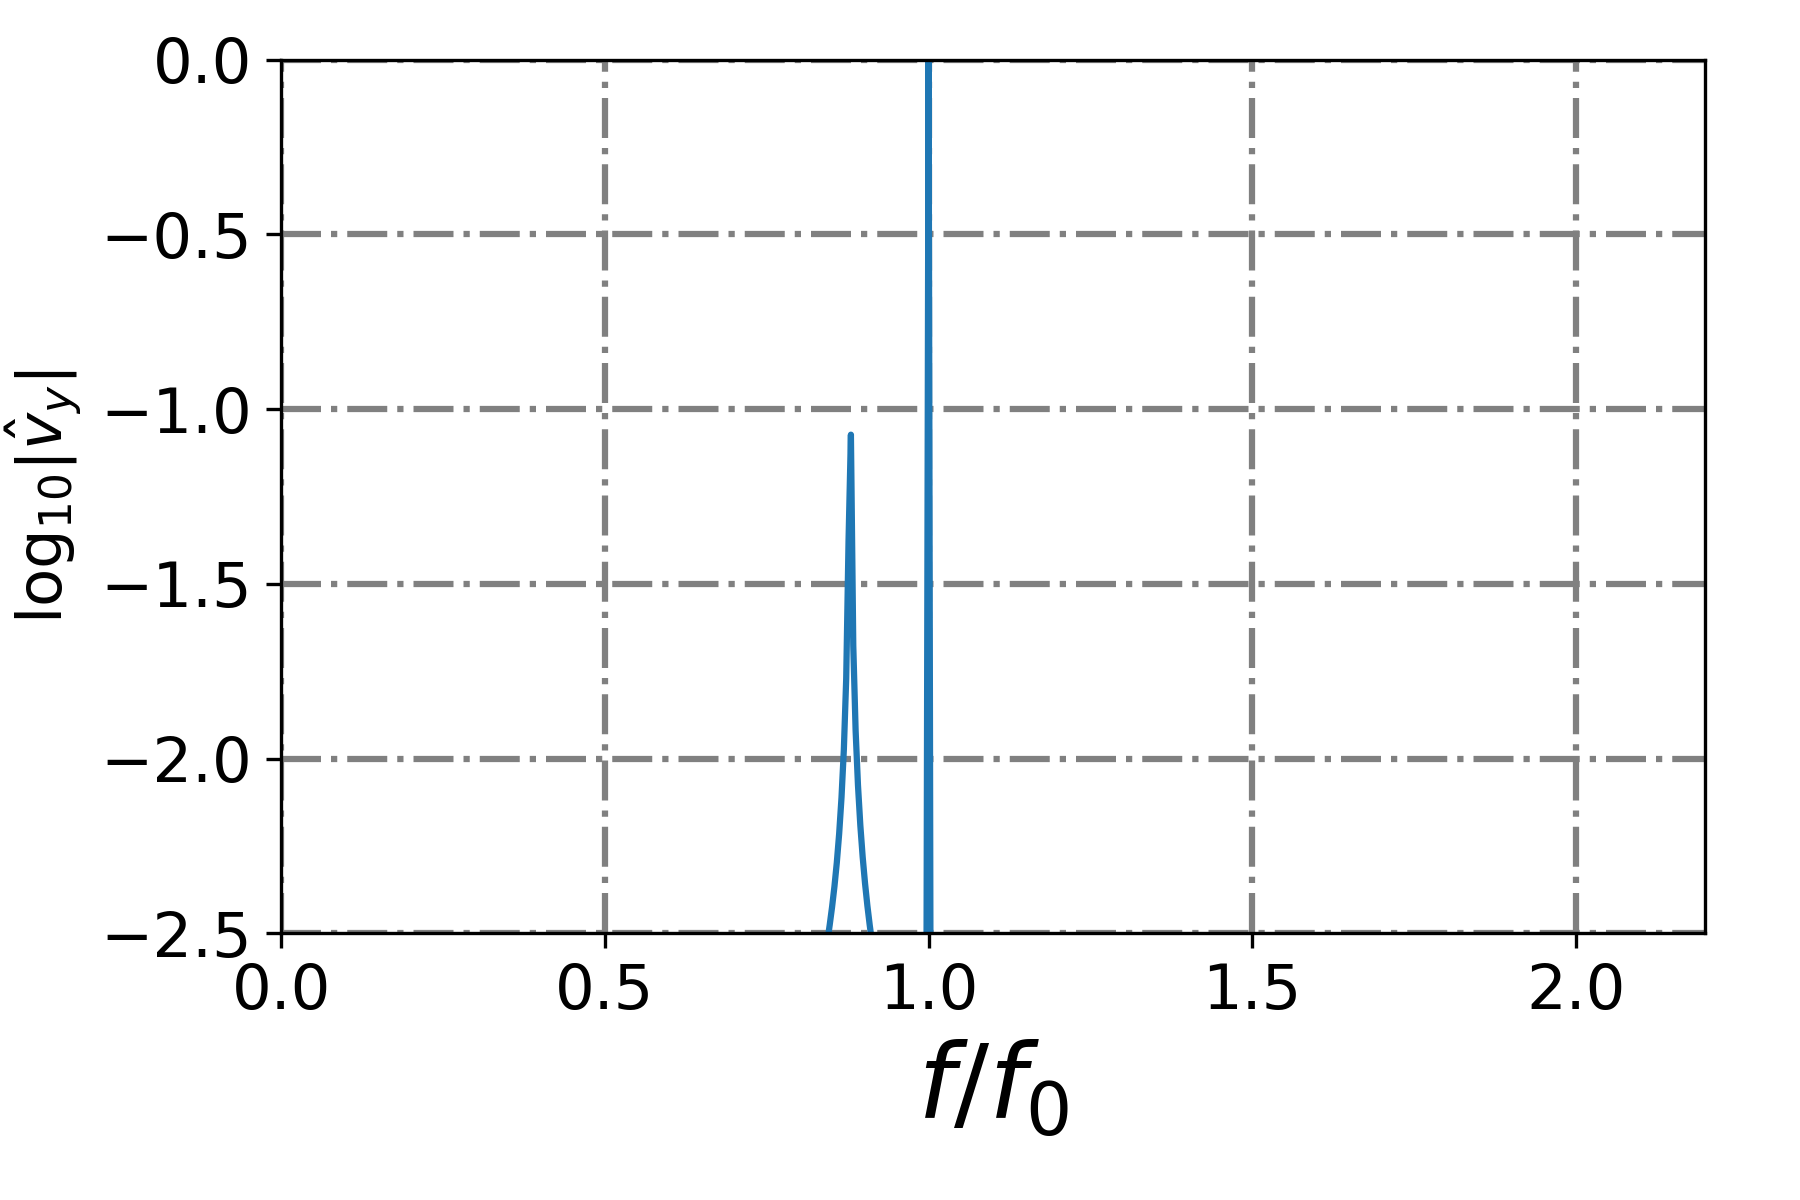
\includegraphics[width=1\textwidth]{pics/H40L60N1ap02dp20w1p58w2p66Biharm/spectrumX36p4Y8p0.png}
        \caption{Спектр}
    \end{subfigure}
    \begin{subfigure}[с]{0.45\textwidth}
        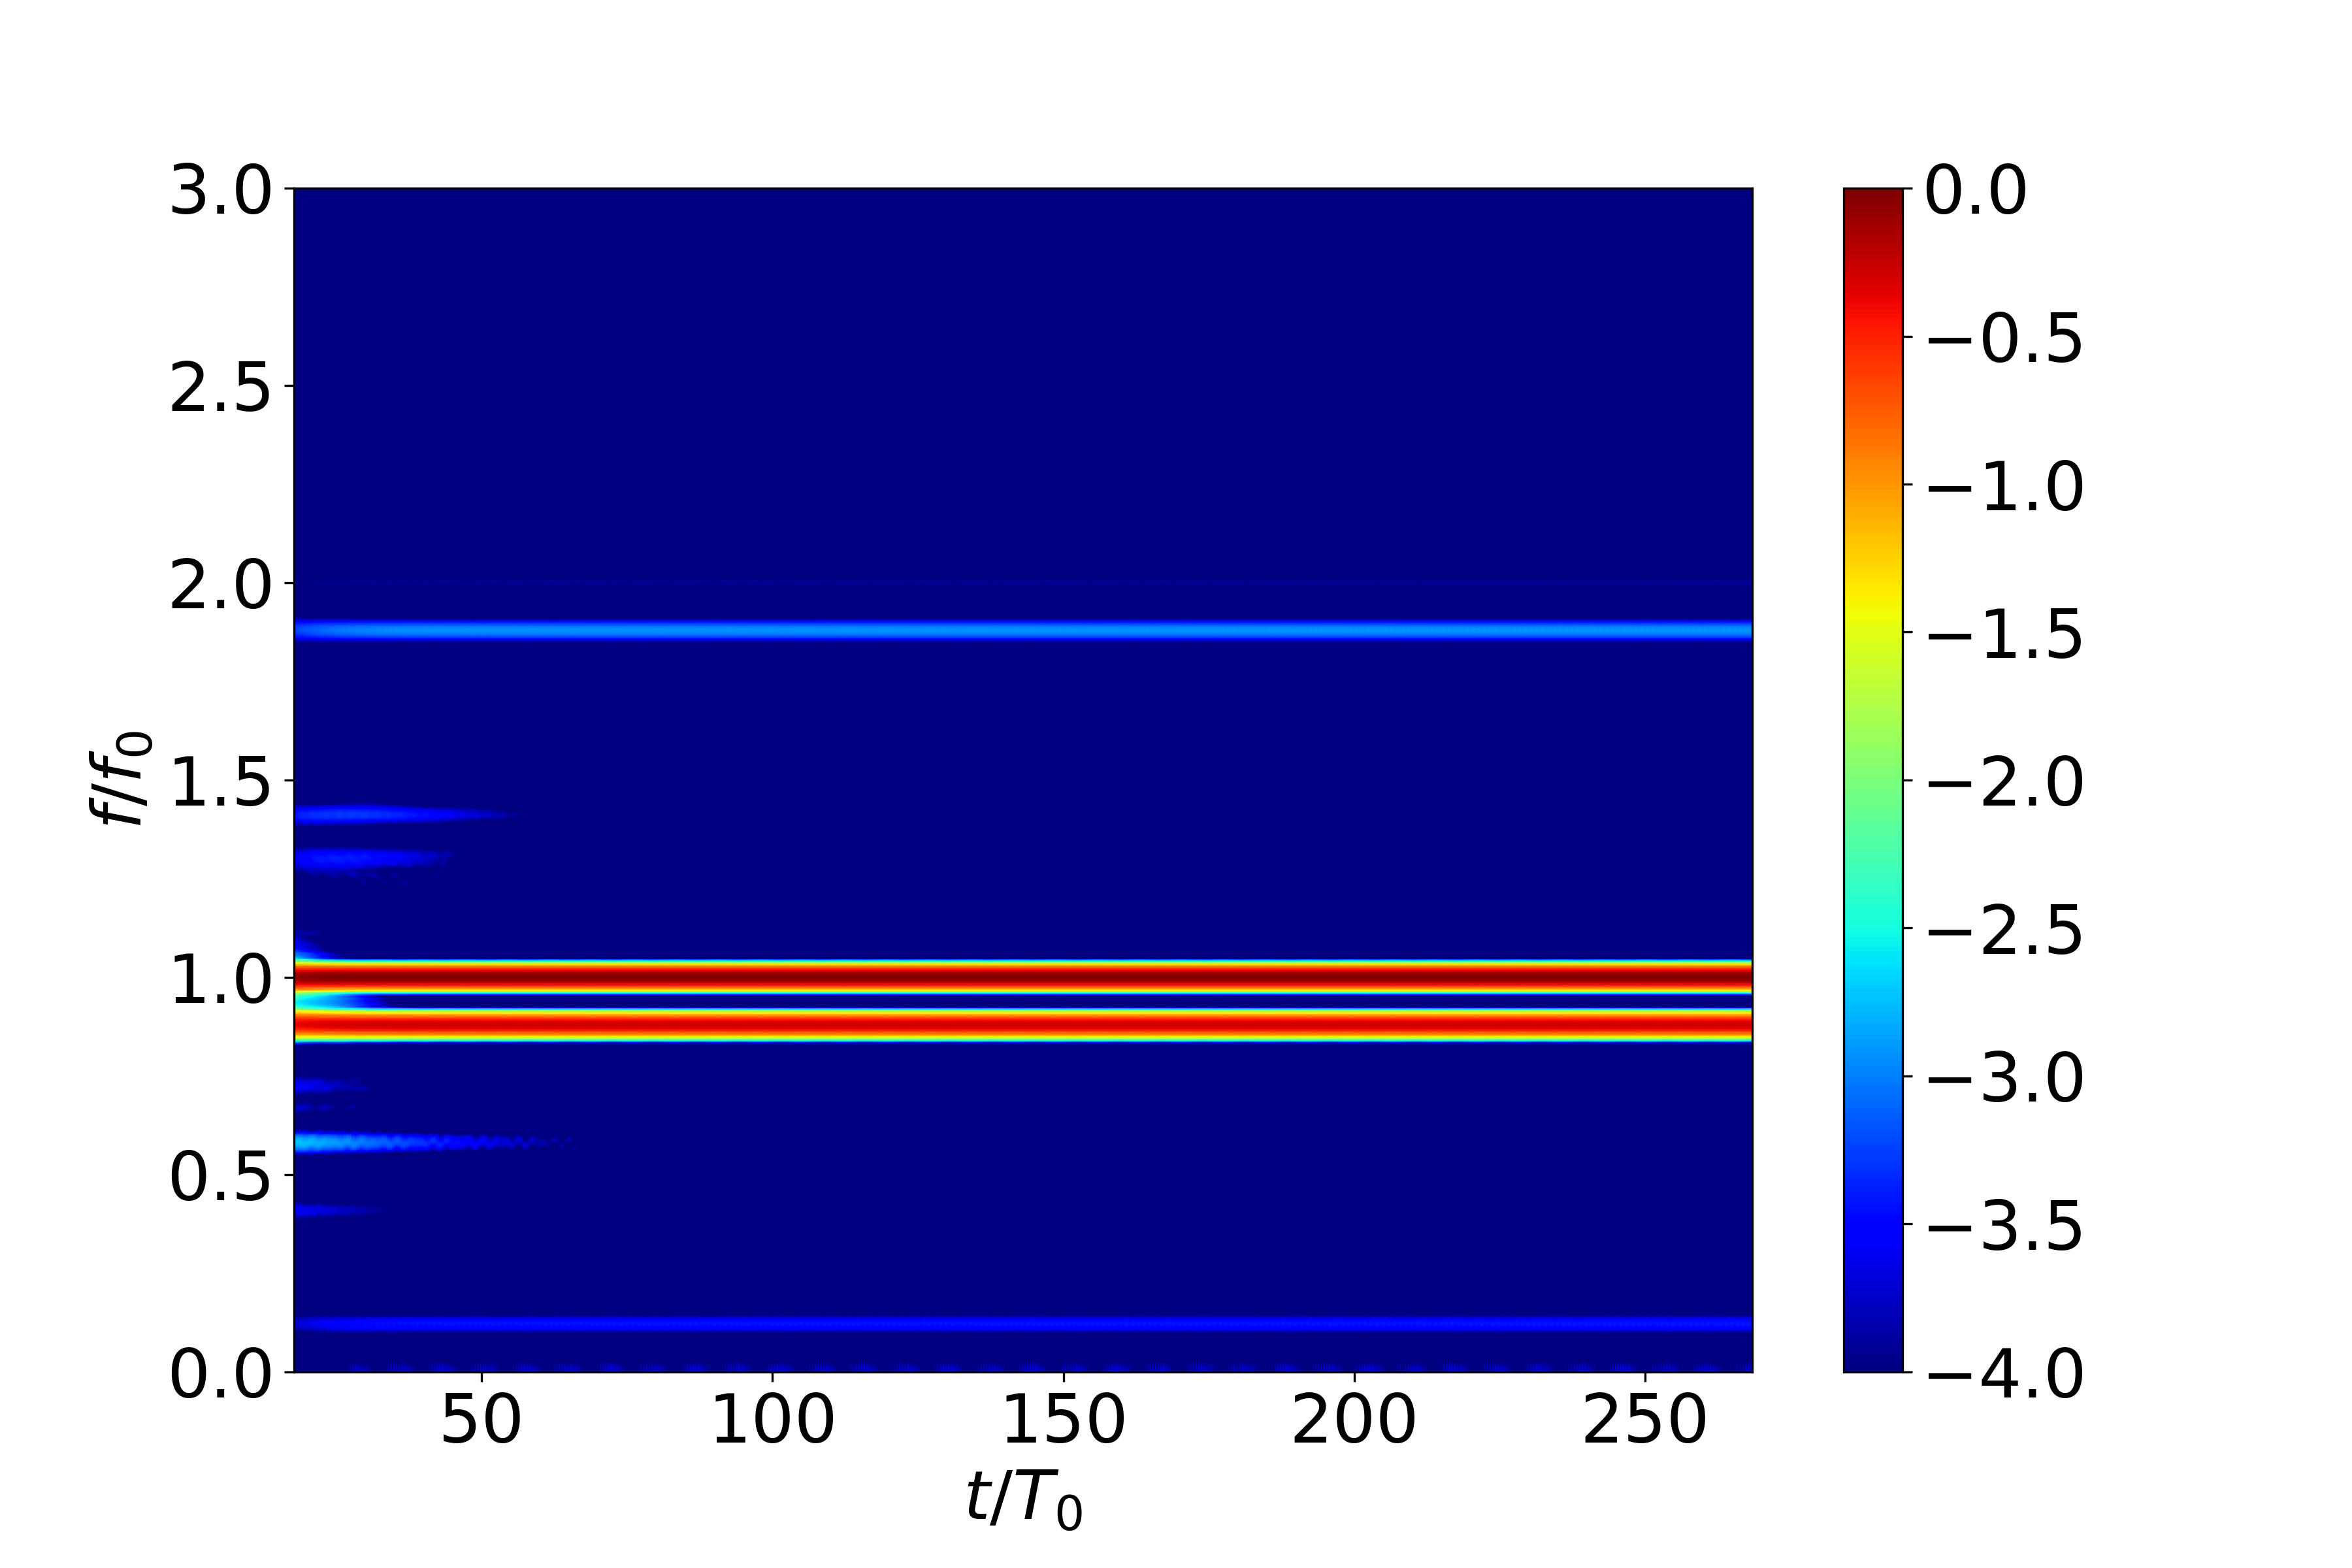
\includegraphics[width=1\textwidth]{pics/H40L60N1ap02dp20w1p58w2p66Biharm/TFspectrumX36p4Y8p0N768.png}
        \caption{Частотно-временная диаграмма}
    \end{subfigure}
    \caption{Результаты количественного исследования характеристик течения стратифицированной жидкости в трапециевидном резервуаре при внешнем воздействии с двумя разнесенными частотами $\omega_1/N=0.58$,  $\omega_2/N=0.66$. Черной линией  на графиках вертикальной скорости и кинетической энергии показана огибающая амплитуды колебаний волнпородуктора.}
    \label{fig:biharmVyamp02}
\end{figure}

Совпадение частот означает, что амплитуда колебаний удваивается значение $a=0.05$ cm. При $a=0.1$ на рисунке \ref{fig:Vyamp1} наблюдается неустойчивость этот режим характеризуется россыпью частот на спектре и частотно-временной диаграмме.

\begin{figure}
	\centering
	\begin{subfigure}[с]{0.45\textwidth}
	    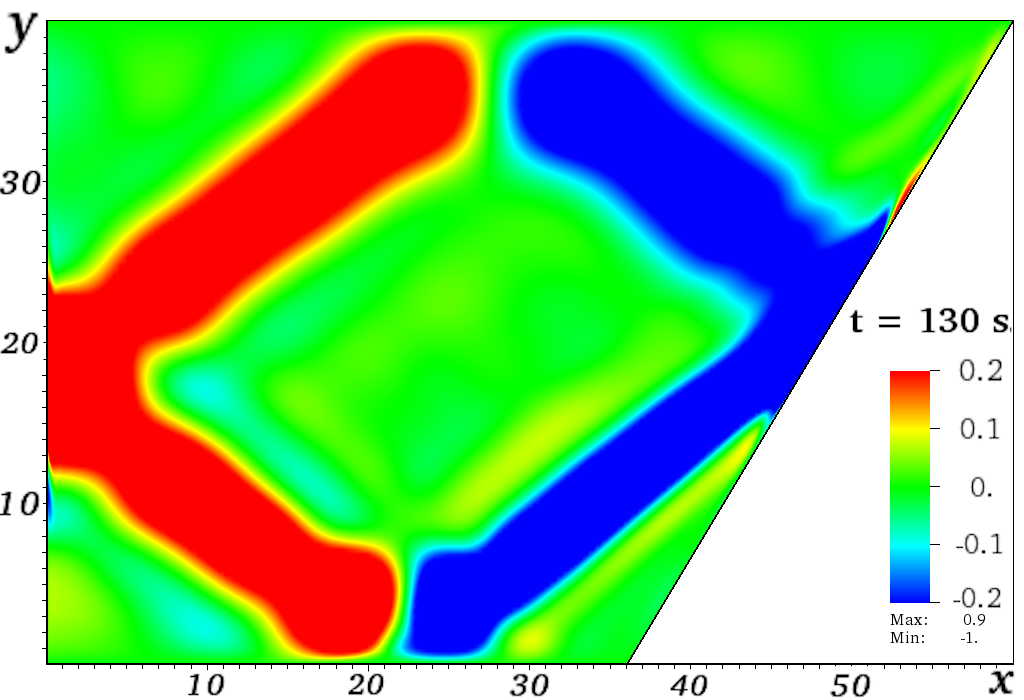
\includegraphics[width=1\textwidth]{pics/H40L60N1ap10dp20w0p63/2DH40L60N1ap10dp20w0p63Vyn00012.png}
	    \caption{Поле вертикальной скорости при образовании аттрактора}
	\end{subfigure}
	\begin{subfigure}[с]{0.45\textwidth}
	    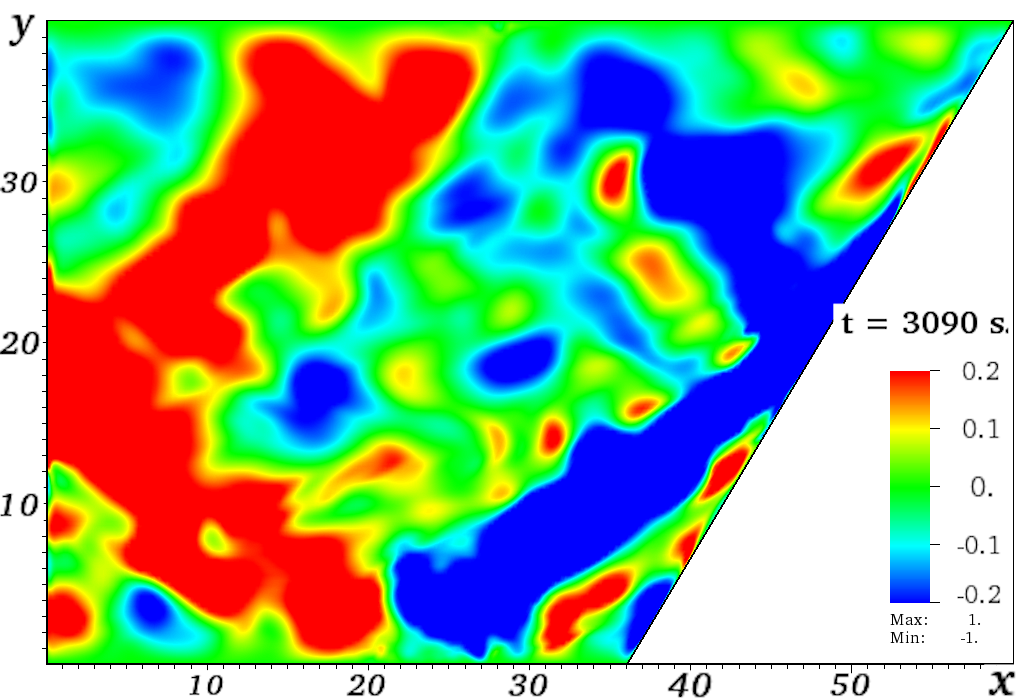
\includegraphics[width=1\textwidth]{pics/H40L60N1ap10dp20w0p63/2DH40L60N1ap10dp20w0p63Vyn00308.png}
	    \caption{Поле вертикальной скорости при образовании неустойчивостей}
	\end{subfigure}
	\par
	\begin{subfigure}[с]{0.45\textwidth}
	    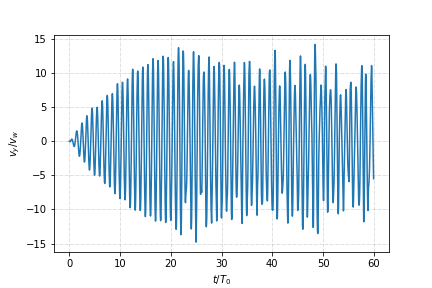
\includegraphics[width=1\textwidth]{pics/H40L60N1ap10dp20w0p63/vyX35p6Y11p3t1200.png}
	    \caption{зависимость скорости в середине первого луча аттрактора от времени}
	\end{subfigure}
	\begin{subfigure}[с]{0.45\textwidth}
	    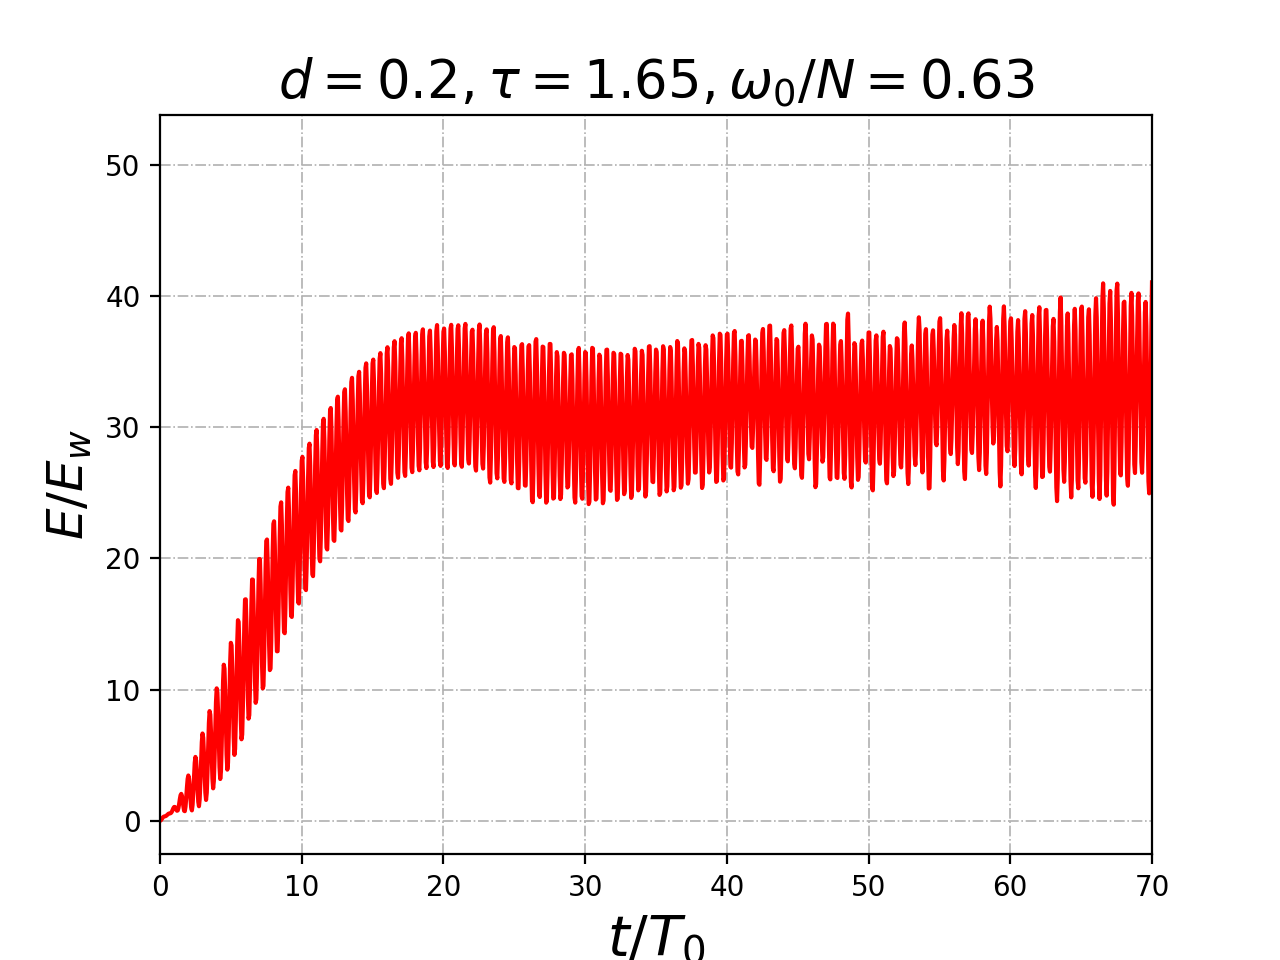
\includegraphics[width=1\textwidth]{pics/H40L60N1ap10dp20w0p63/2D36x36DiagramH40L60N1ap10dp20w0p63totKEnonDim.png}
	    \caption{Зависимость кинетической энергии от времени}
	\end{subfigure}
	\par
	\begin{subfigure}[с]{0.45\textwidth}
	    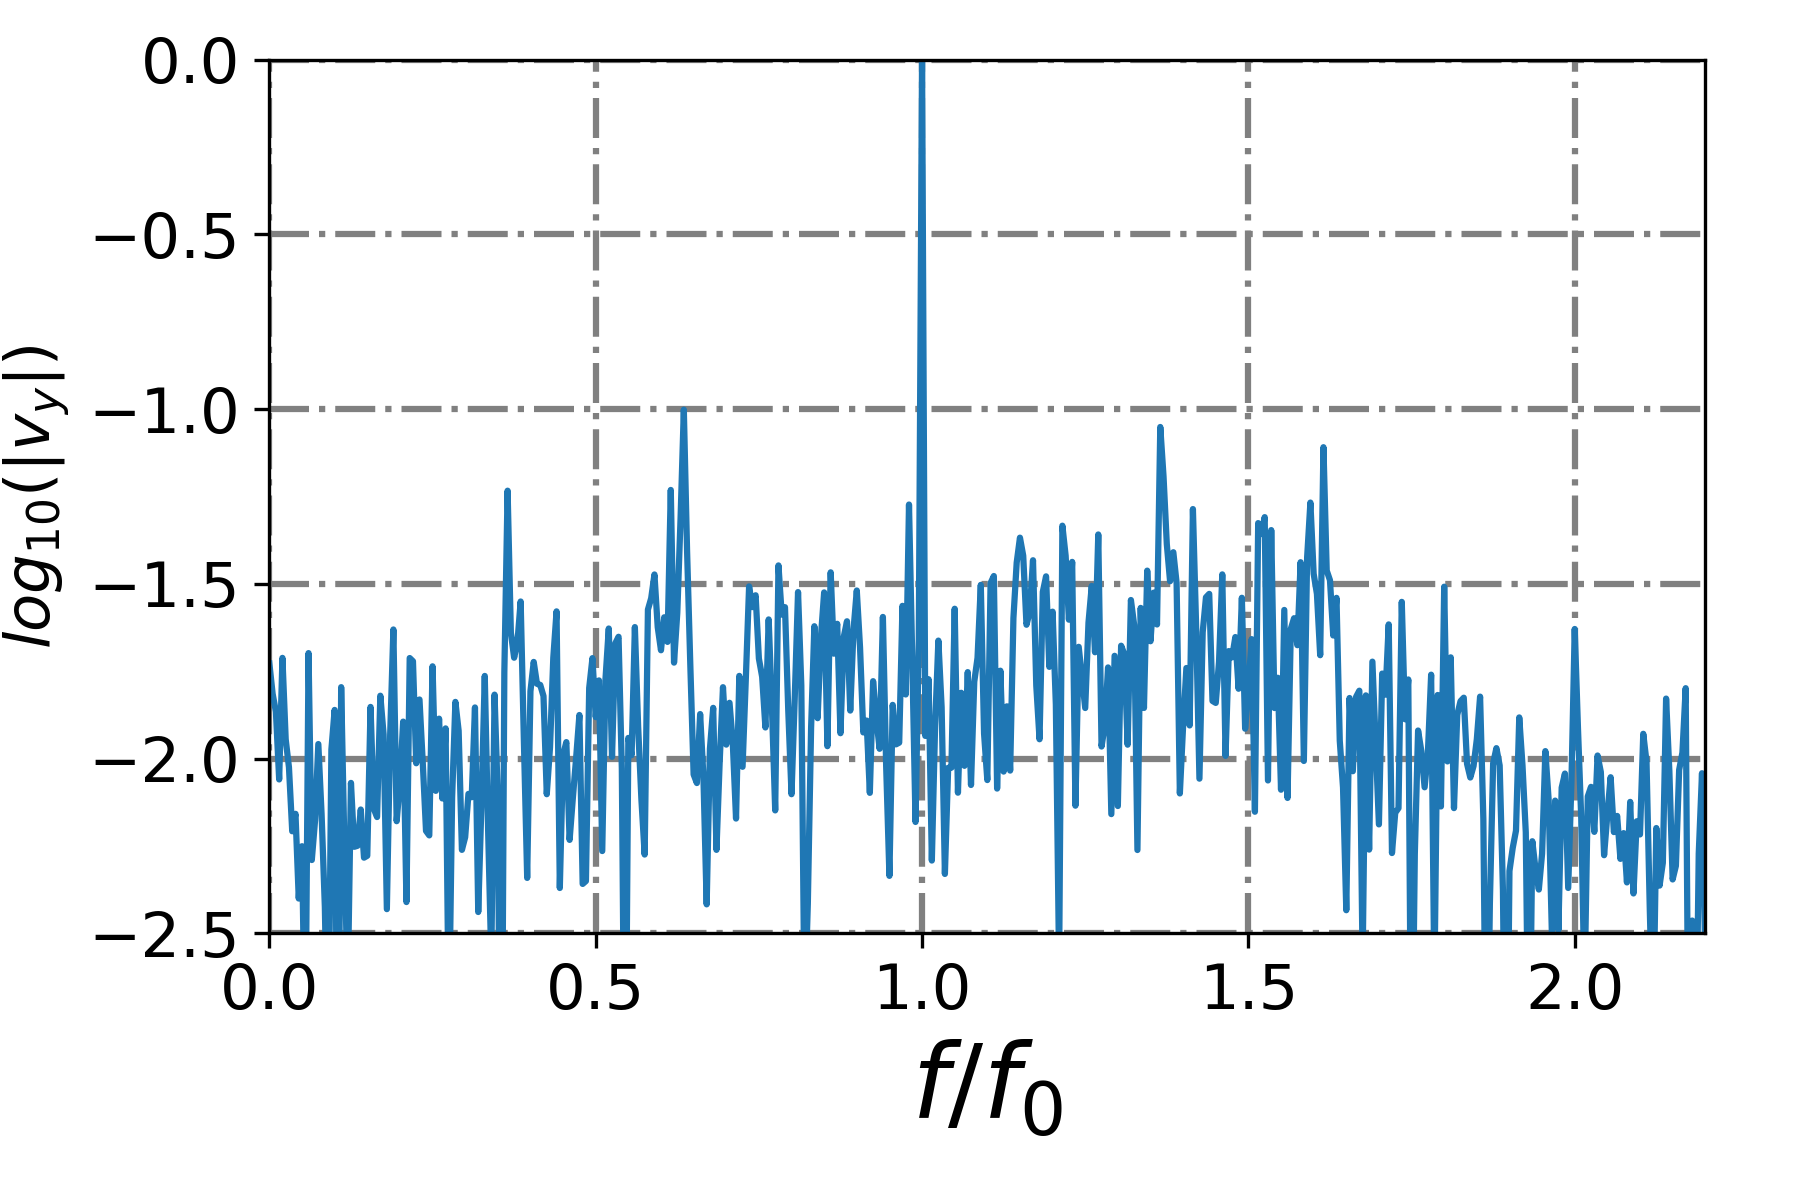
\includegraphics[width=1\textwidth]{pics/H40L60N1ap10dp20w0p63/spectrumX35p6Y11p2n4000.png}
	    \caption{Частотный спектр скорости}
	\end{subfigure}
	\begin{subfigure}[с]{0.45\textwidth}
	    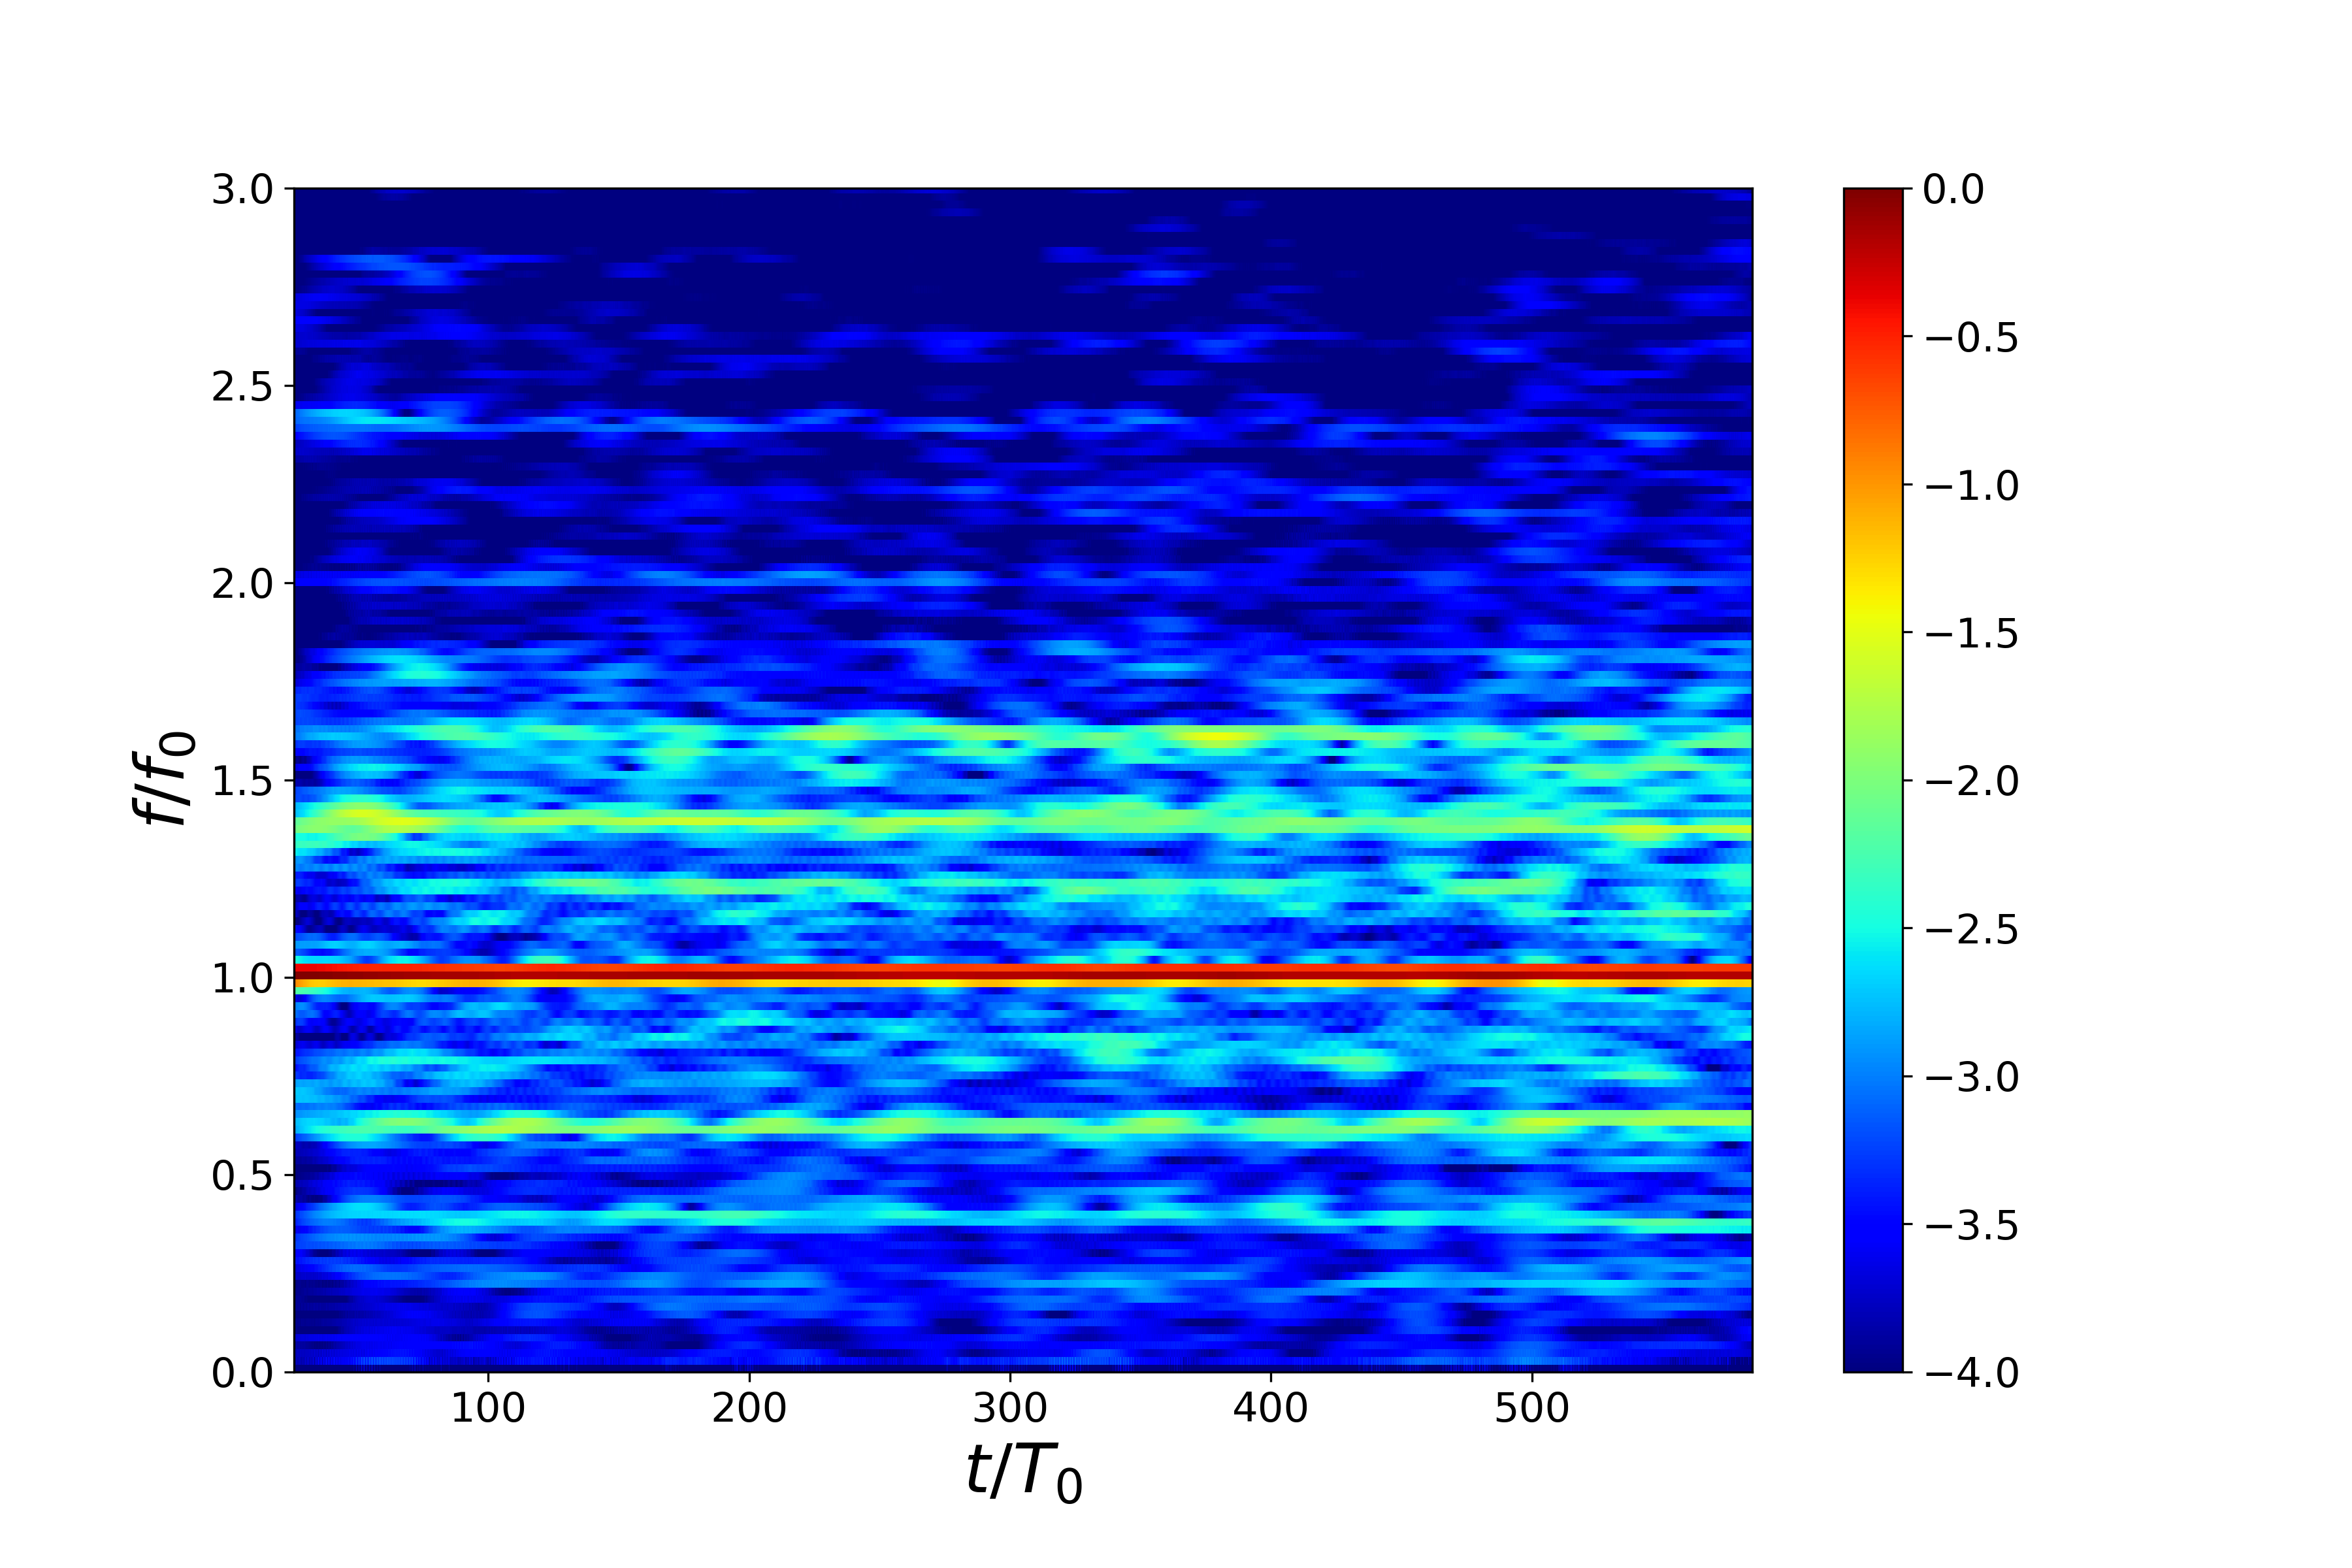
\includegraphics[width=1\textwidth]{pics/H40L60N1ap10dp20w0p63/TFspectrumX35p6Y11p2N1024.png}
	    \caption{Частотно-временная диаграмма}
	\end{subfigure}
	\label{fig:Vyamp1-1}
	\caption{Количественное исследования аттрактора с совпадающими частотами и образование неустойчивости}
	\label{fig:Vyamp1}
\end{figure}

Последующие режимы это попытка постепенно приблизить две частоты друг к другу и зафиксировать момент возникновения неустойчивости в зависимости от близости частот друг к другу. На рисунке \ref{fig:biharmVyap005-1} представлена картина течения при относительной разности частот в 0.05. При этом режиме наблюдаются дочерние волны как на изображении с вертикальной компонентой скорости, спектре так и на частотно временной диаграмме. При этом на последней наблюдаются  амплитудные <<всплески>>. Это объясняется совпадением фаз двух волновых процессов.

\begin{figure}
  \centering
  \begin{subfigure}[с]{0.45\textwidth}
    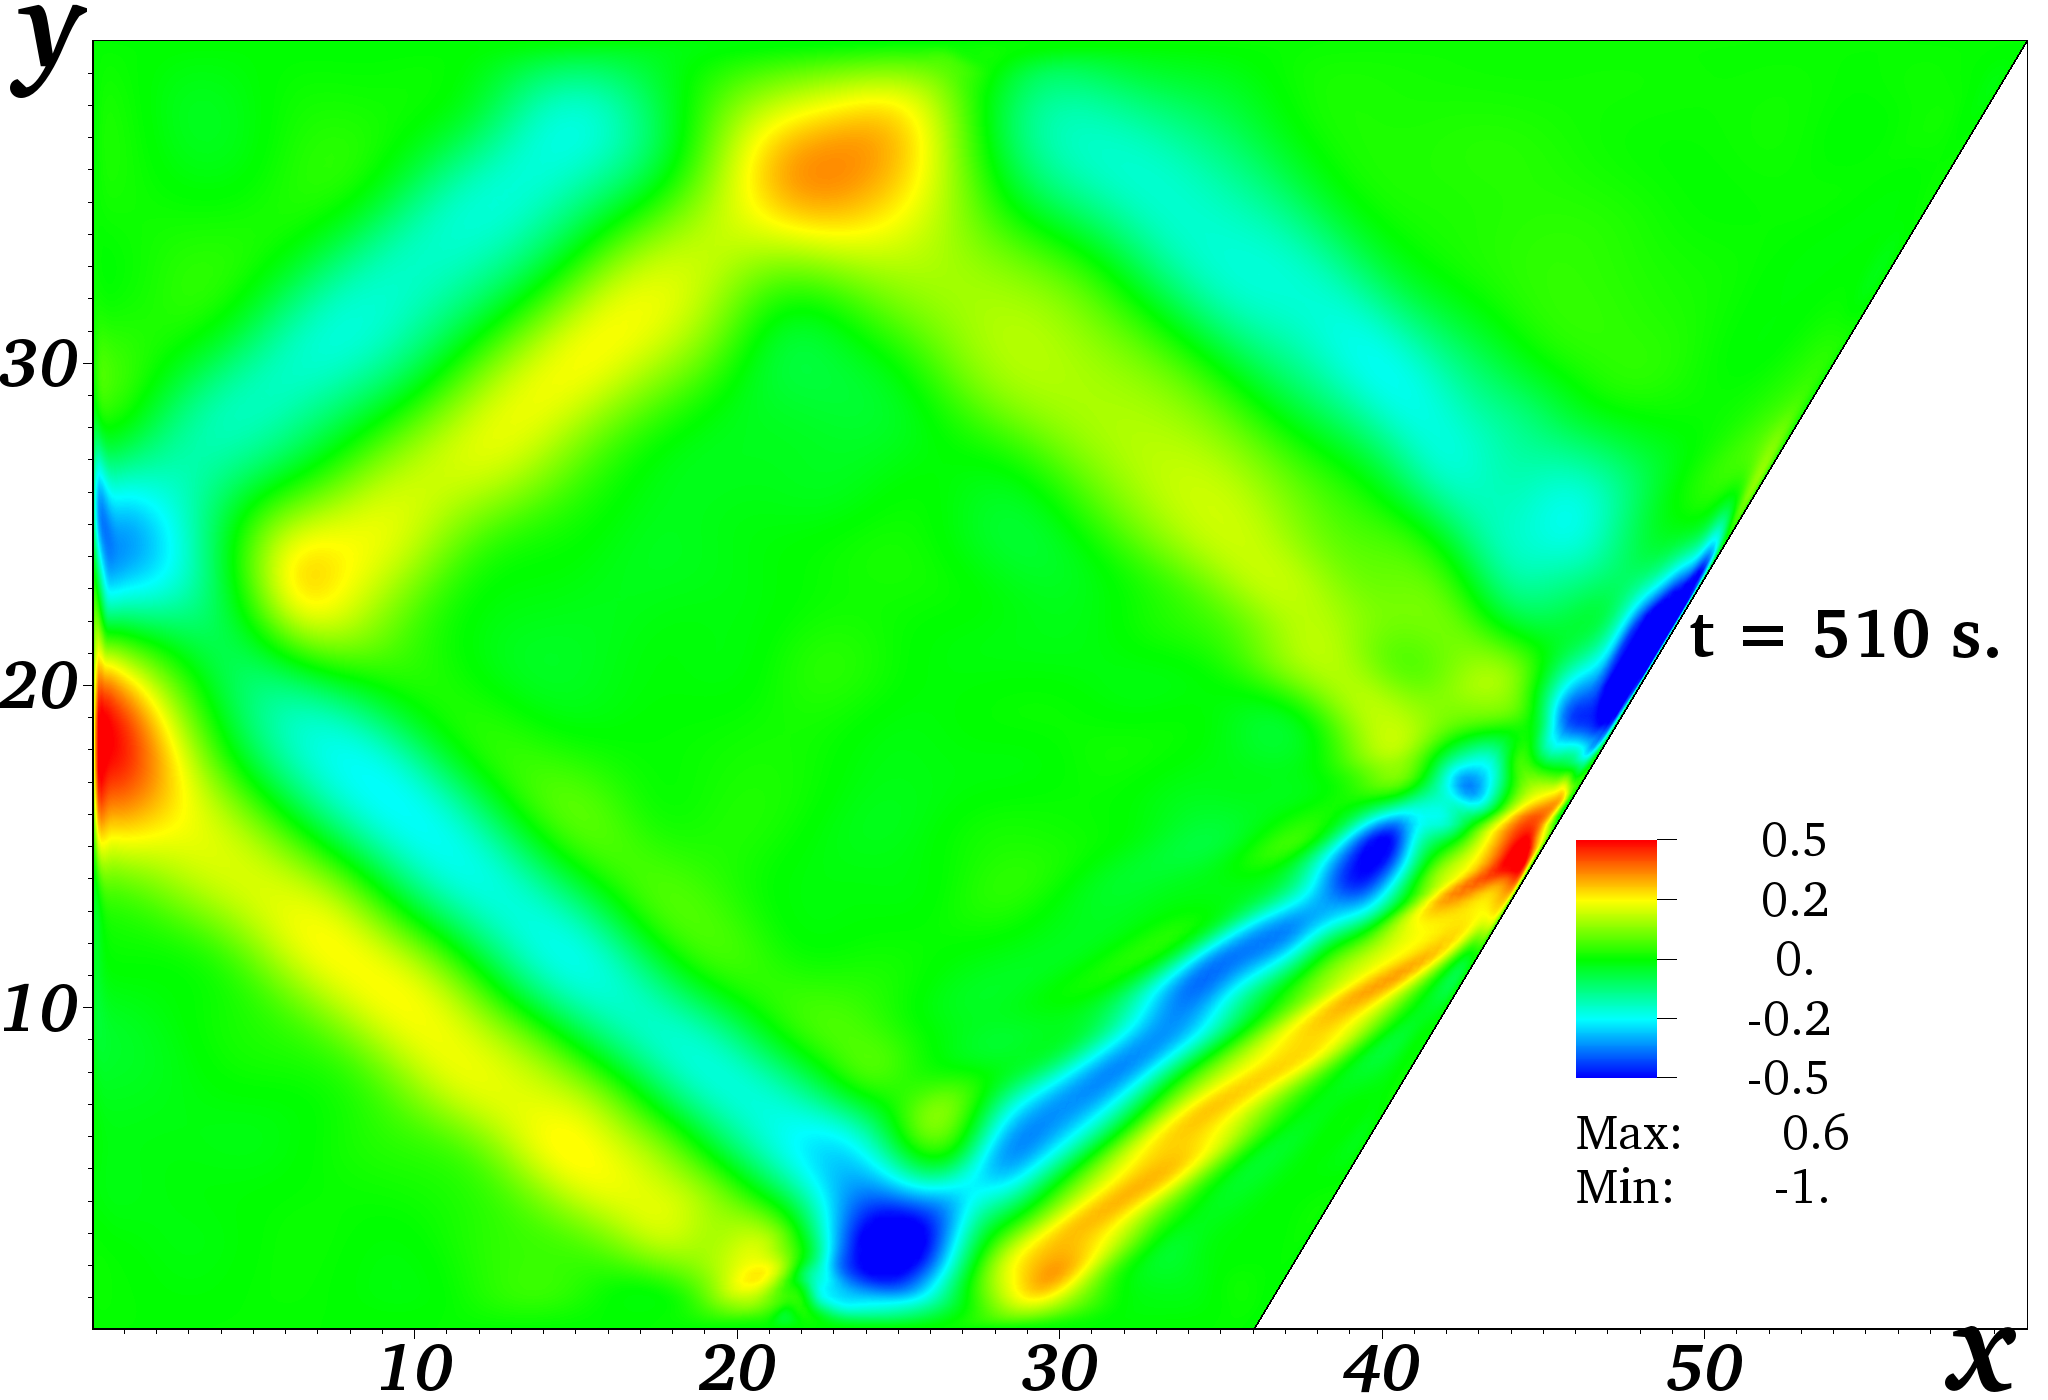
\includegraphics[width=1\textwidth]{pics/H40L60N1ap05dp20w1p63Deltawp05Biharm/2D36x36DiagramH40L60N1ap05dp20w0p63Deltawp3315BiharmVyn01019.png}
    \caption{Вертикальная компонента скорости при формировании аттрактора}
  \end{subfigure}
  \begin{subfigure}[с]{0.45\textwidth}
    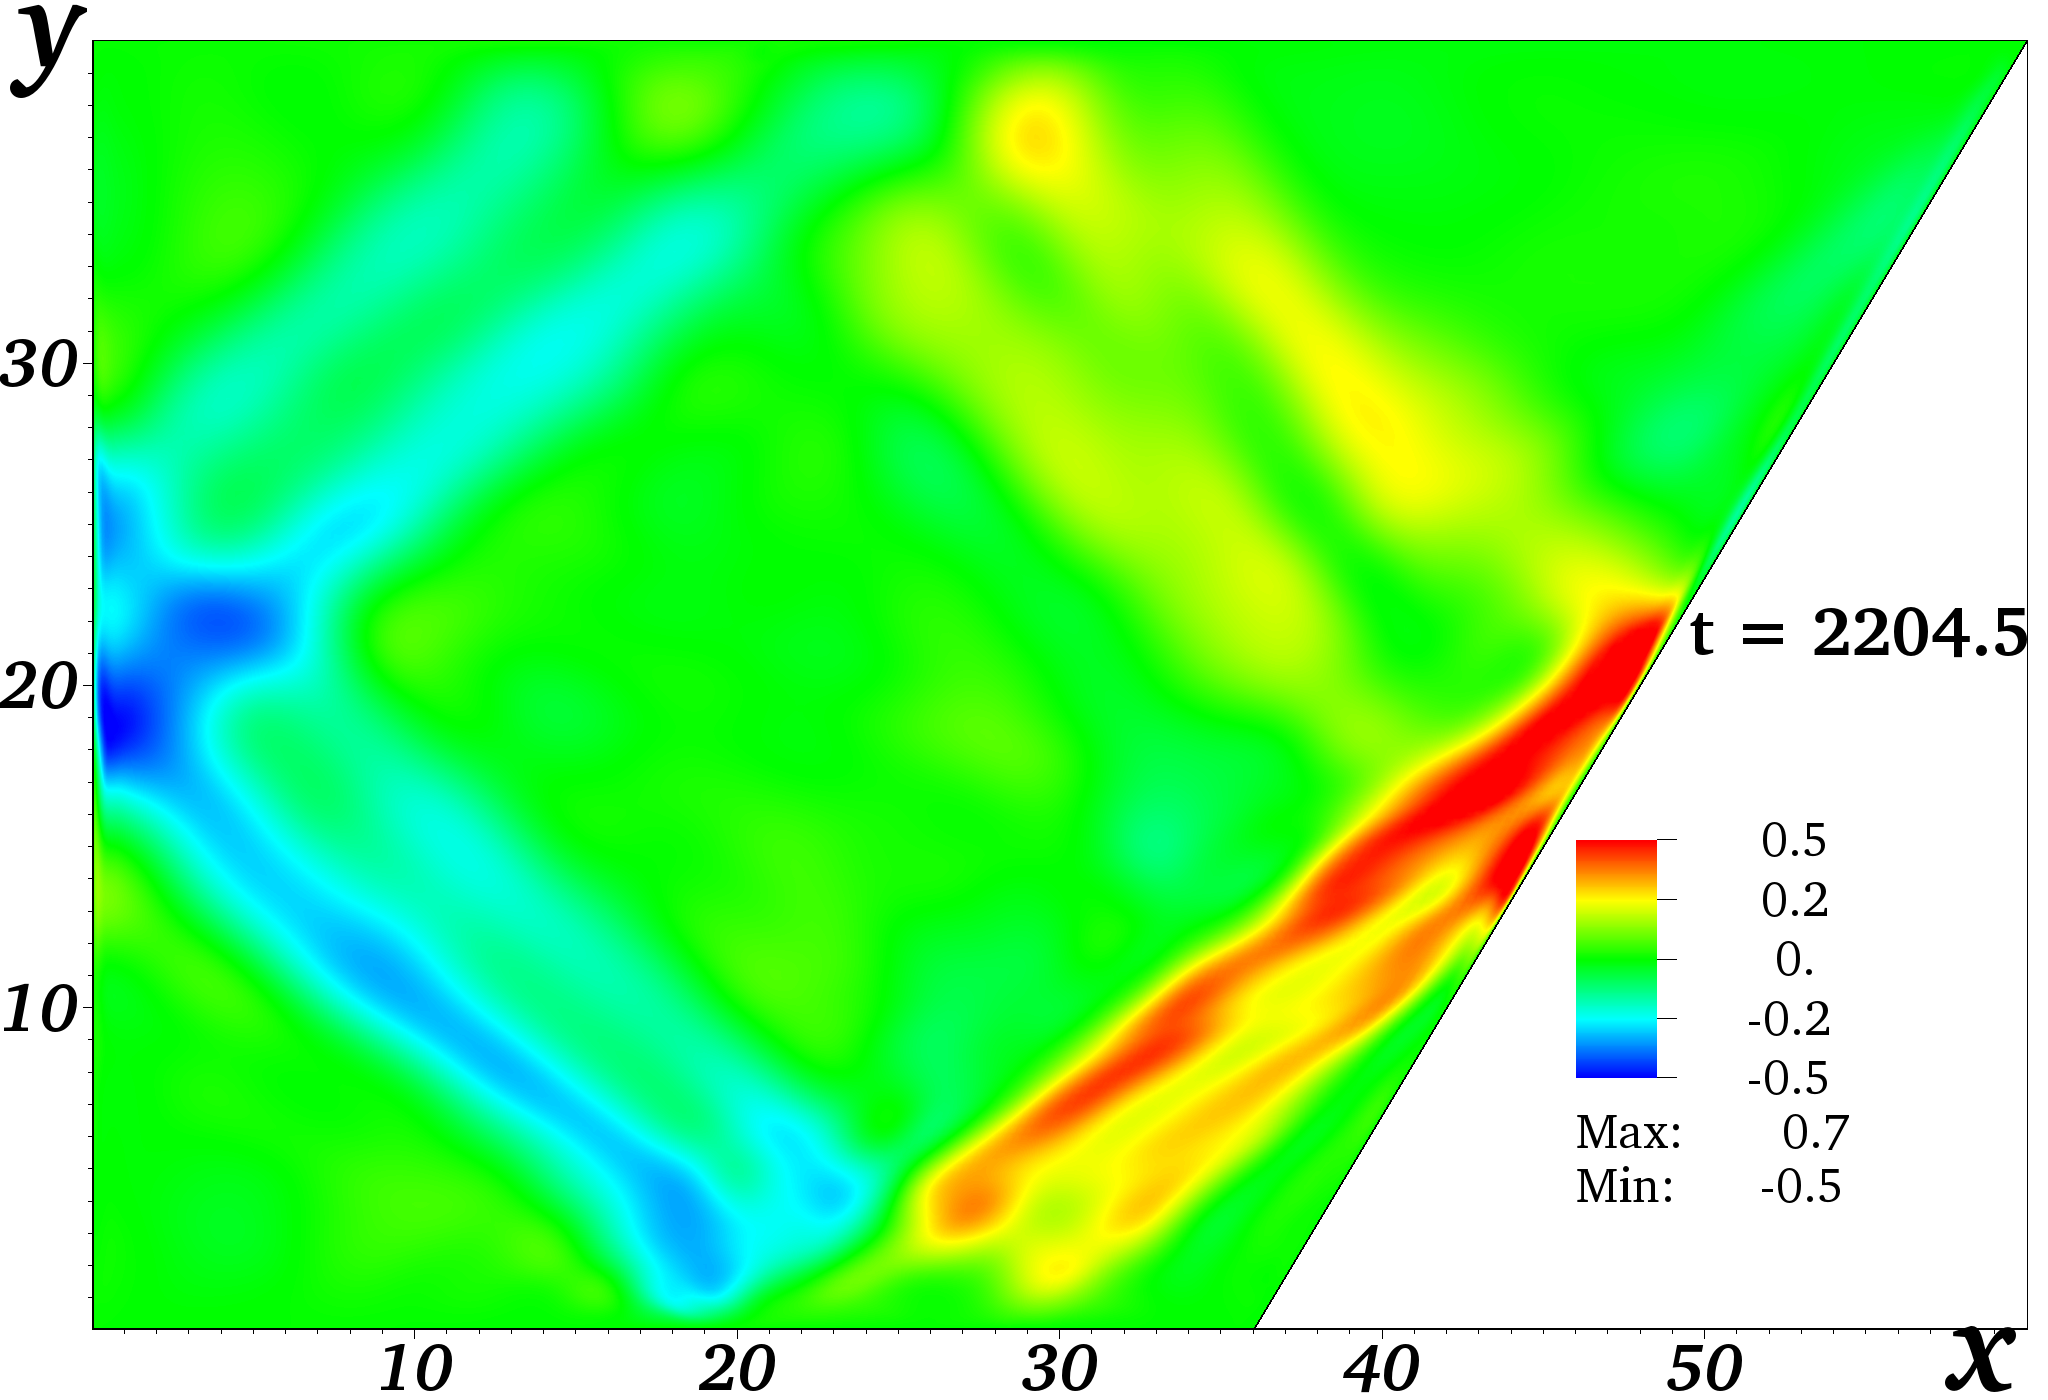
\includegraphics[width=1\textwidth]{pics/H40L60N1ap05dp20w1p63Deltawp05Biharm/2D36x36DiagramH40L60N1ap05dp20w0p63Deltawp3315BiharmVyn04408.png}
    \caption{Вертикальная компонента скорости при установлении аттрактора}
  \end{subfigure}
  \par
  \begin{subfigure}[с]{0.45\textwidth}
    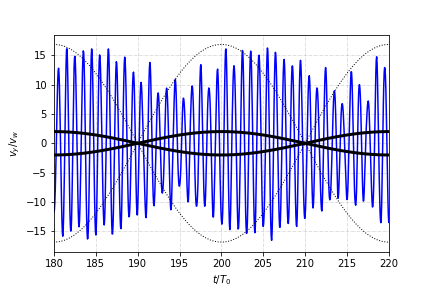
\includegraphics[width=1\textwidth]{pics/H40L60N1ap05dp20w1p63Deltawp05Biharm/vyX35p57Y11p27t4412.png}
    \caption{Вертикальная скорость}
  \end{subfigure}
  \begin{subfigure}[с]{0.45\textwidth}
    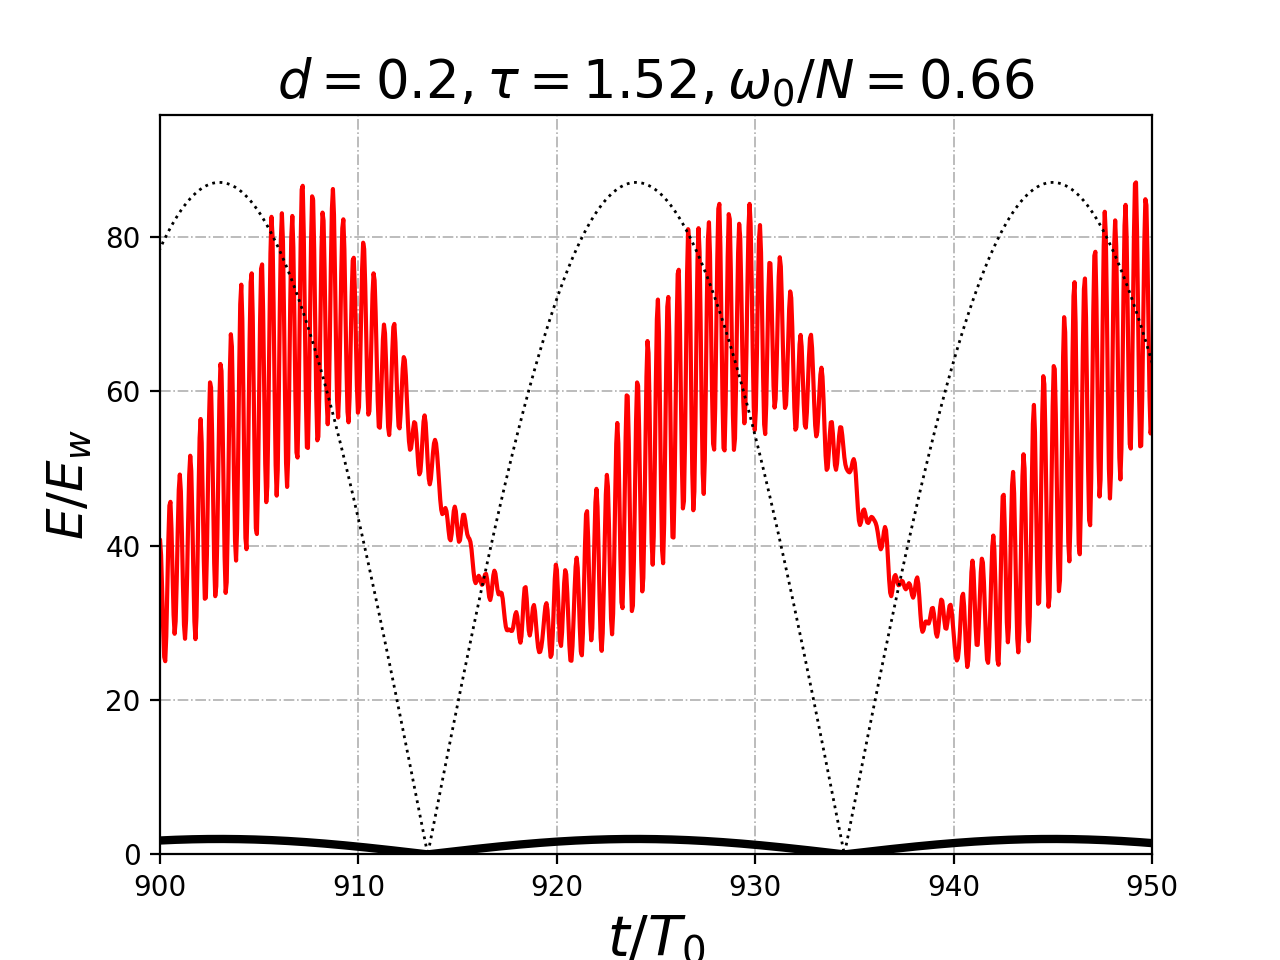
\includegraphics[width=1\textwidth]{pics/H40L60N1ap05dp20w1p63Deltawp05Biharm/2D36x36DiagramH40L60N1ap05dp20w1p63Deltawp05BiharmtotKEnonDim.png}
    \caption{Кинетическая энергия}
  \end{subfigure}
  \par
  \begin{subfigure}[с]{0.45\textwidth}
    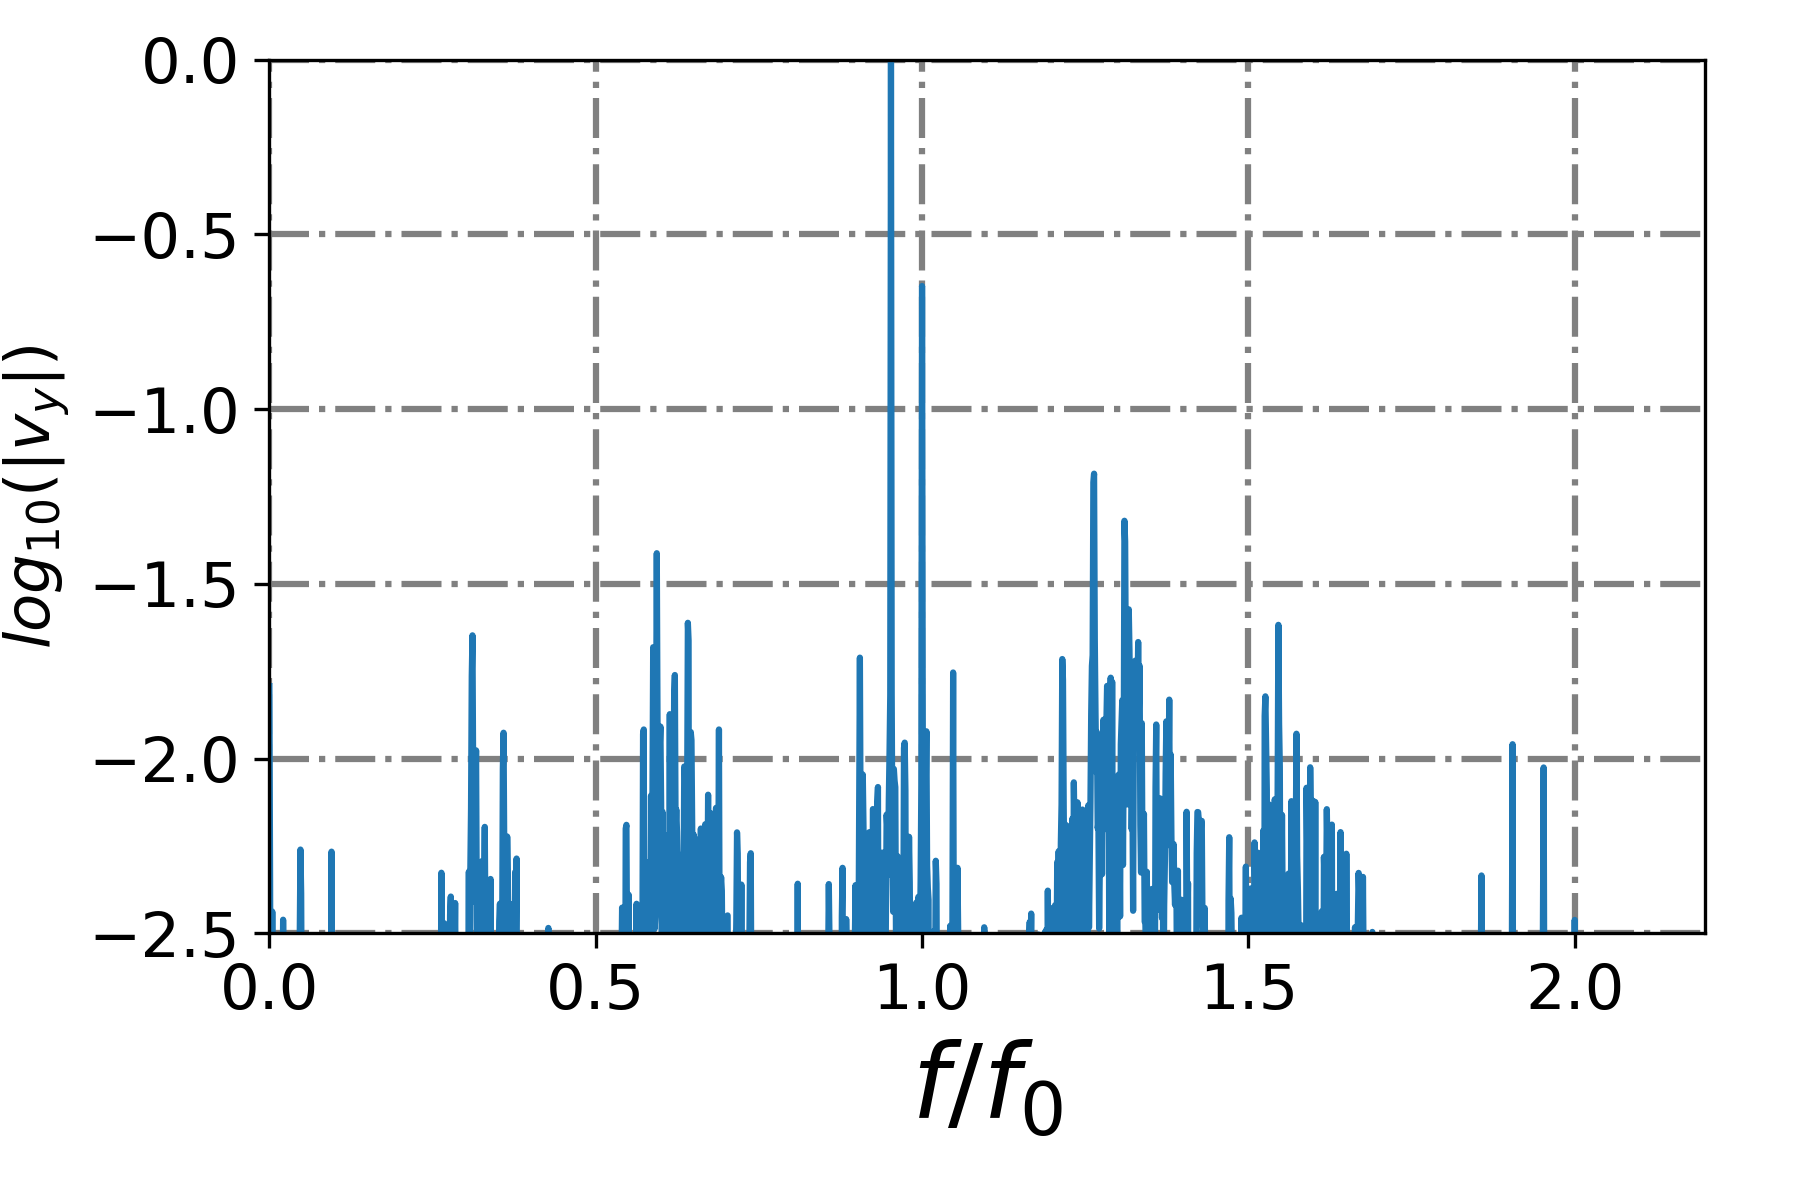
\includegraphics[width=1\textwidth]{pics/H40L60N1ap05dp20w1p63Deltawp05Biharm/spectrumX35p6Y11p2.png}
    \caption{Спектр}
  \end{subfigure}
  \begin{subfigure}[с]{0.45\textwidth}
    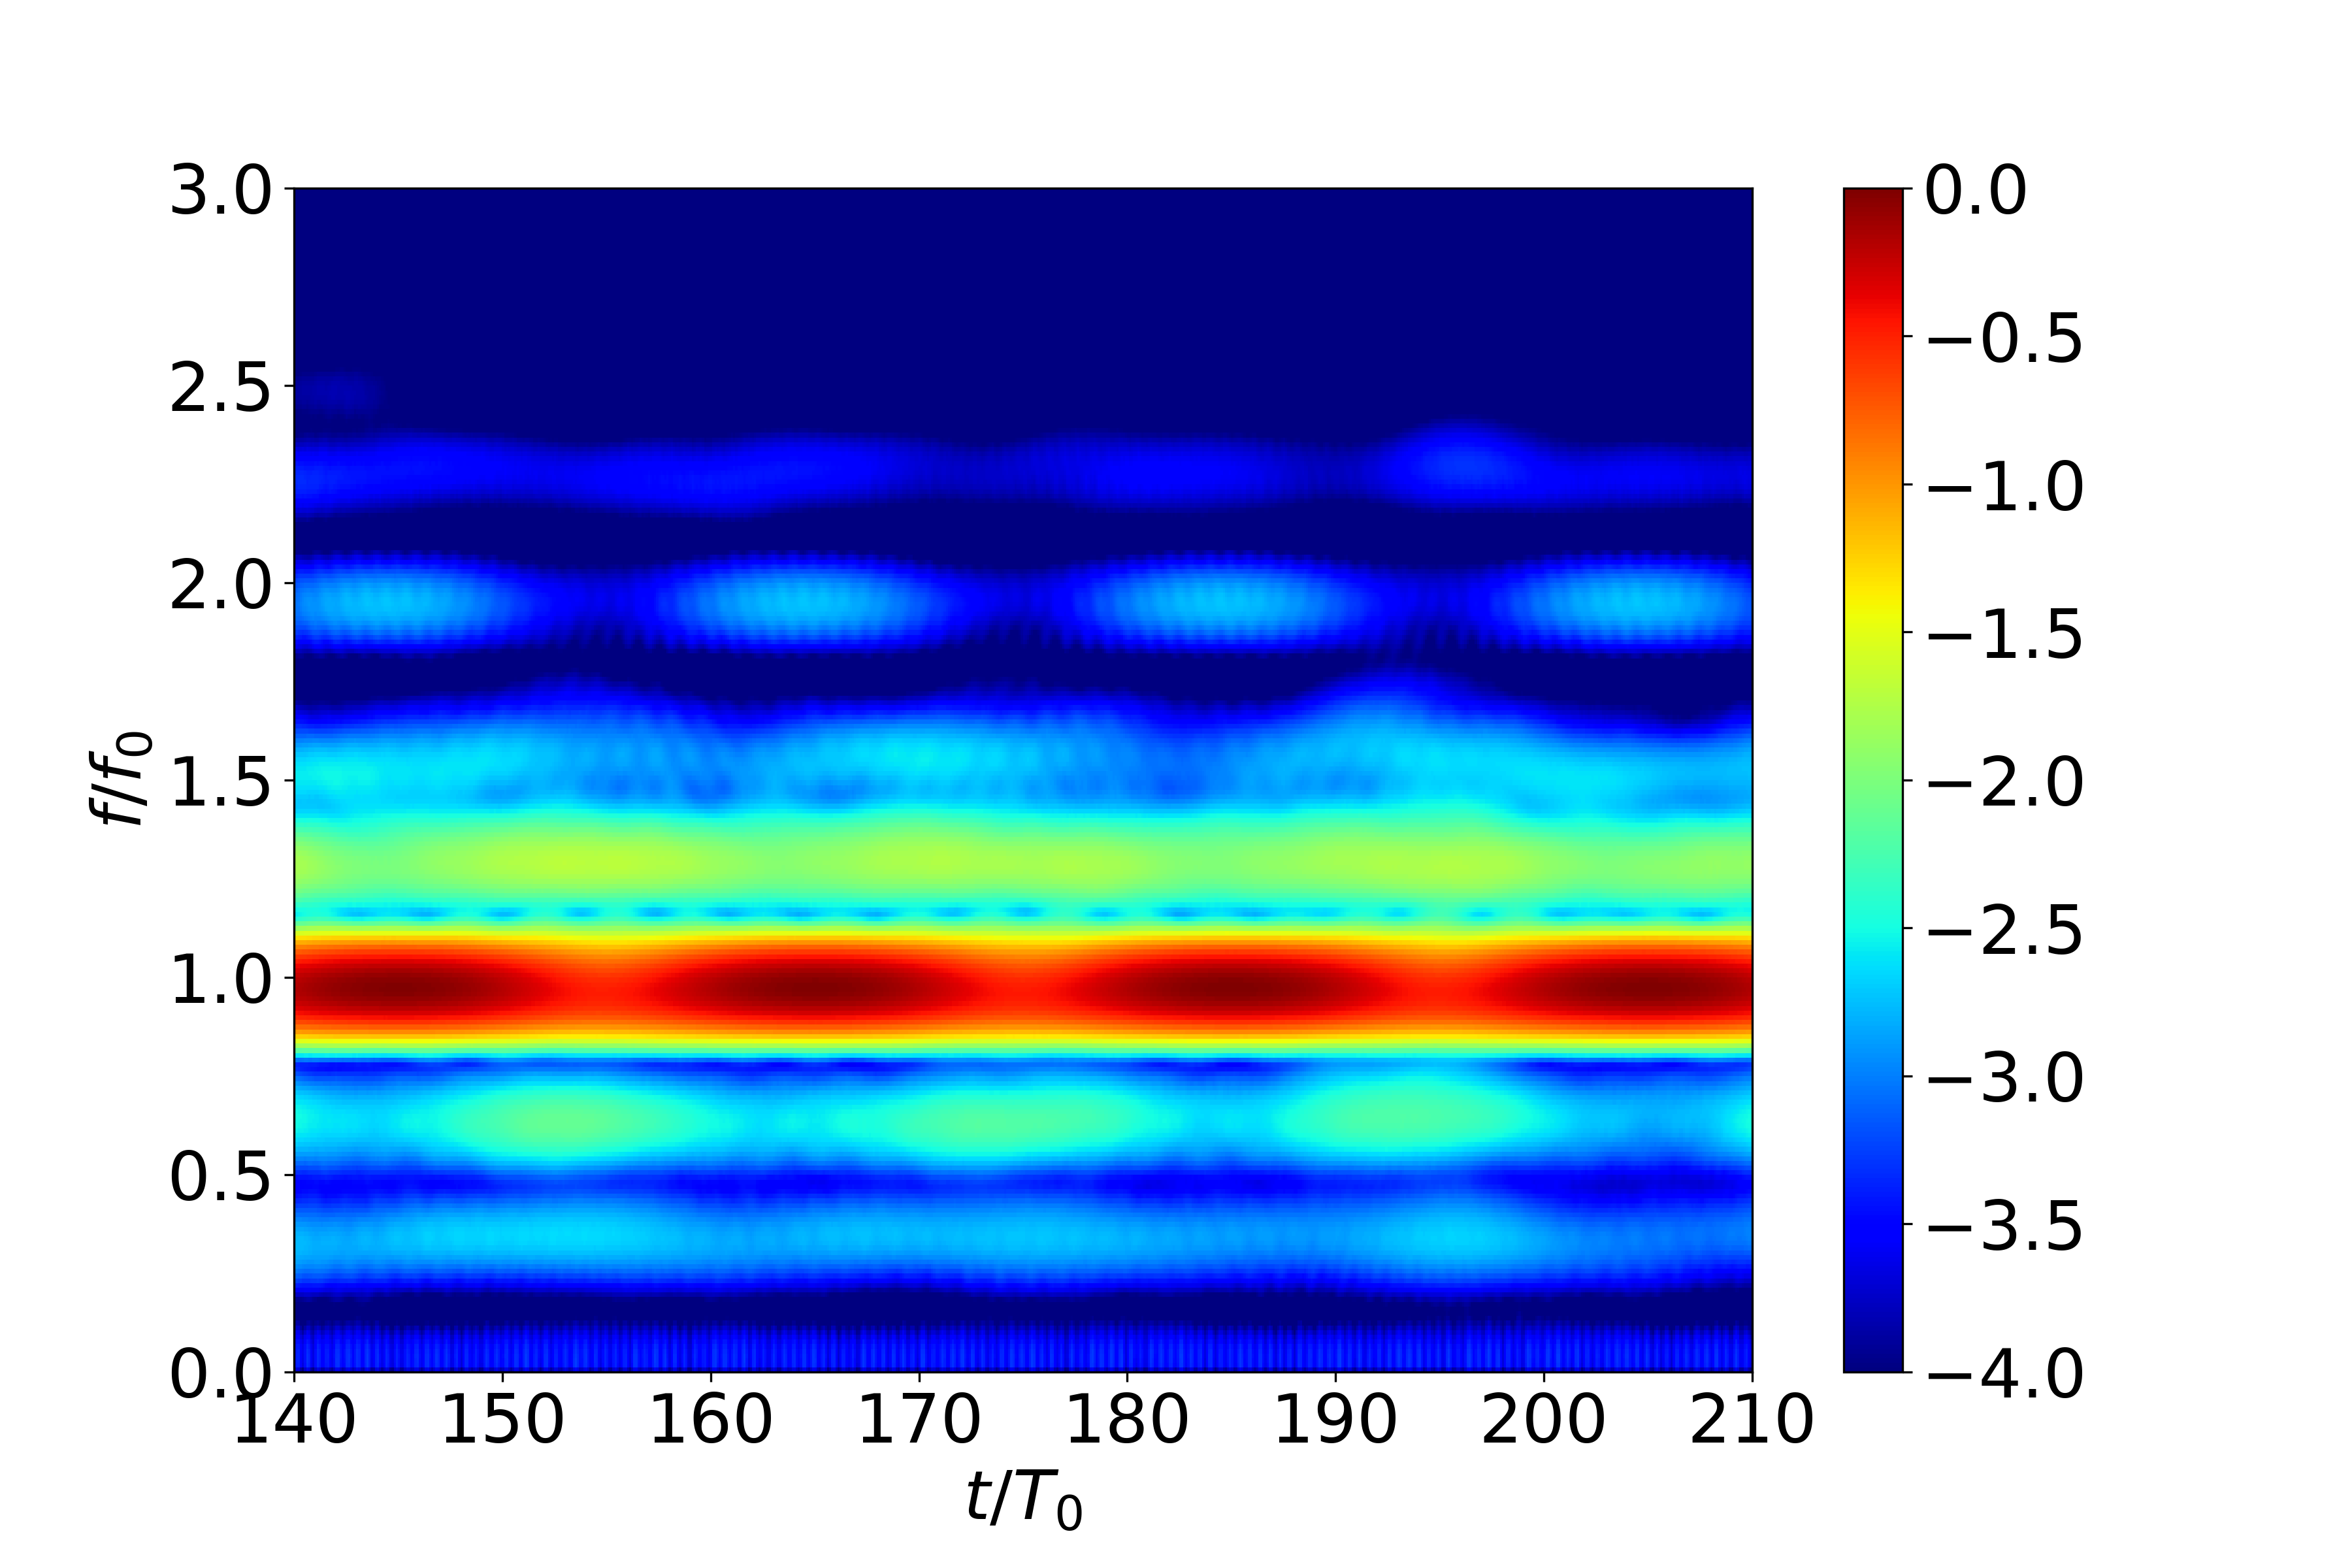
\includegraphics[width=1\textwidth]{pics/H40L60N1ap05dp20w1p63Deltawp05Biharm/TFspectrumX35p6Y11p2N200.png}
    \caption{Частотно-временная диаграмма}
    \label{}
  \end{subfigure}
  \caption{Результаты количественного исследования характеристик течения стратифицированной жидкости в трапециевидном резервуаре при внешнем воздействии с двумя приближенными частотами $\omega_1/N=0.66$ $\omega_2/N=0.68$. Черной линией  на графиках вертикальной скорости и кинетической энергии показана огибающая амплитуды колебаний волнпородуктора.}

  \label{fig:biharmVyap005-1}
\end{figure}

С приближением частот друг к другу(см. рис. \ref{fig:biharmVyap005-2}) появляются дополнительные дочерние волны, но режим успевает стабилизироваться во временной промежуток разности фаз двух частот. 

\begin{figure}
  \centering
  \begin{subfigure}[с]{0.45\textwidth}
    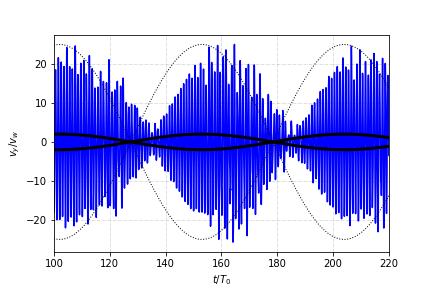
\includegraphics[width=1\textwidth]{pics/H40L60N1ap05dp20w1p63Deltawp02Biharm/vyX35p57Y11p27t4400.png}
    \caption{Вертикальная компонента скорости в зависимости от времени}
  \end{subfigure}
  \begin{subfigure}[с]{0.45\textwidth}
    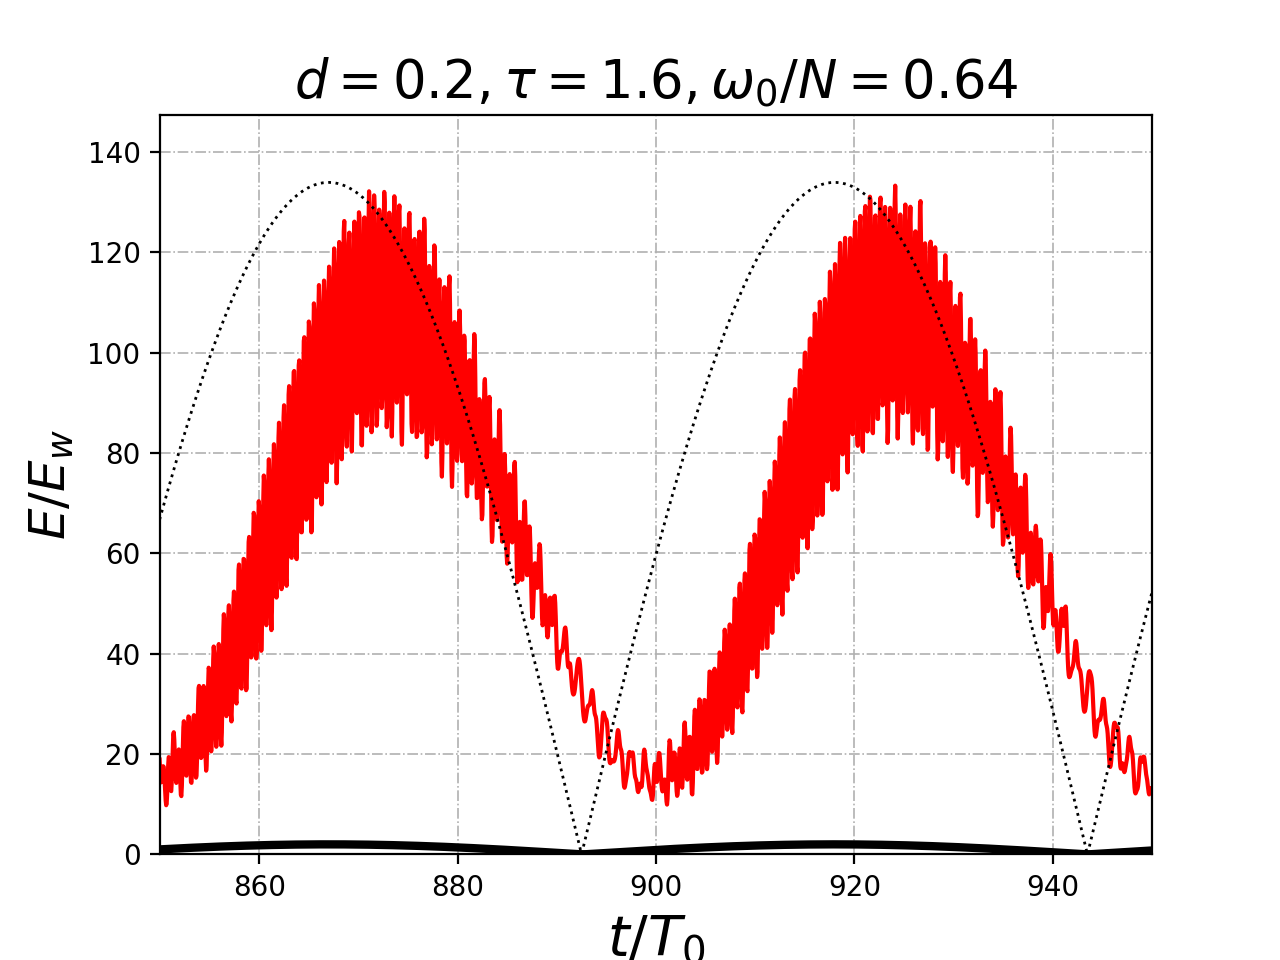
\includegraphics[width=1\textwidth]{pics/H40L60N1ap05dp20w1p63Deltawp02Biharm/2D36x36DiagramH40L60N1ap05dp20w1p63Deltawp02BiharmtotKEnonDim.png}
    \caption{Средняя кинетическая энергия в резервуаре в зависимости от времени}
  \end{subfigure}
  \par
  \begin{subfigure}[с]{0.45\textwidth}
    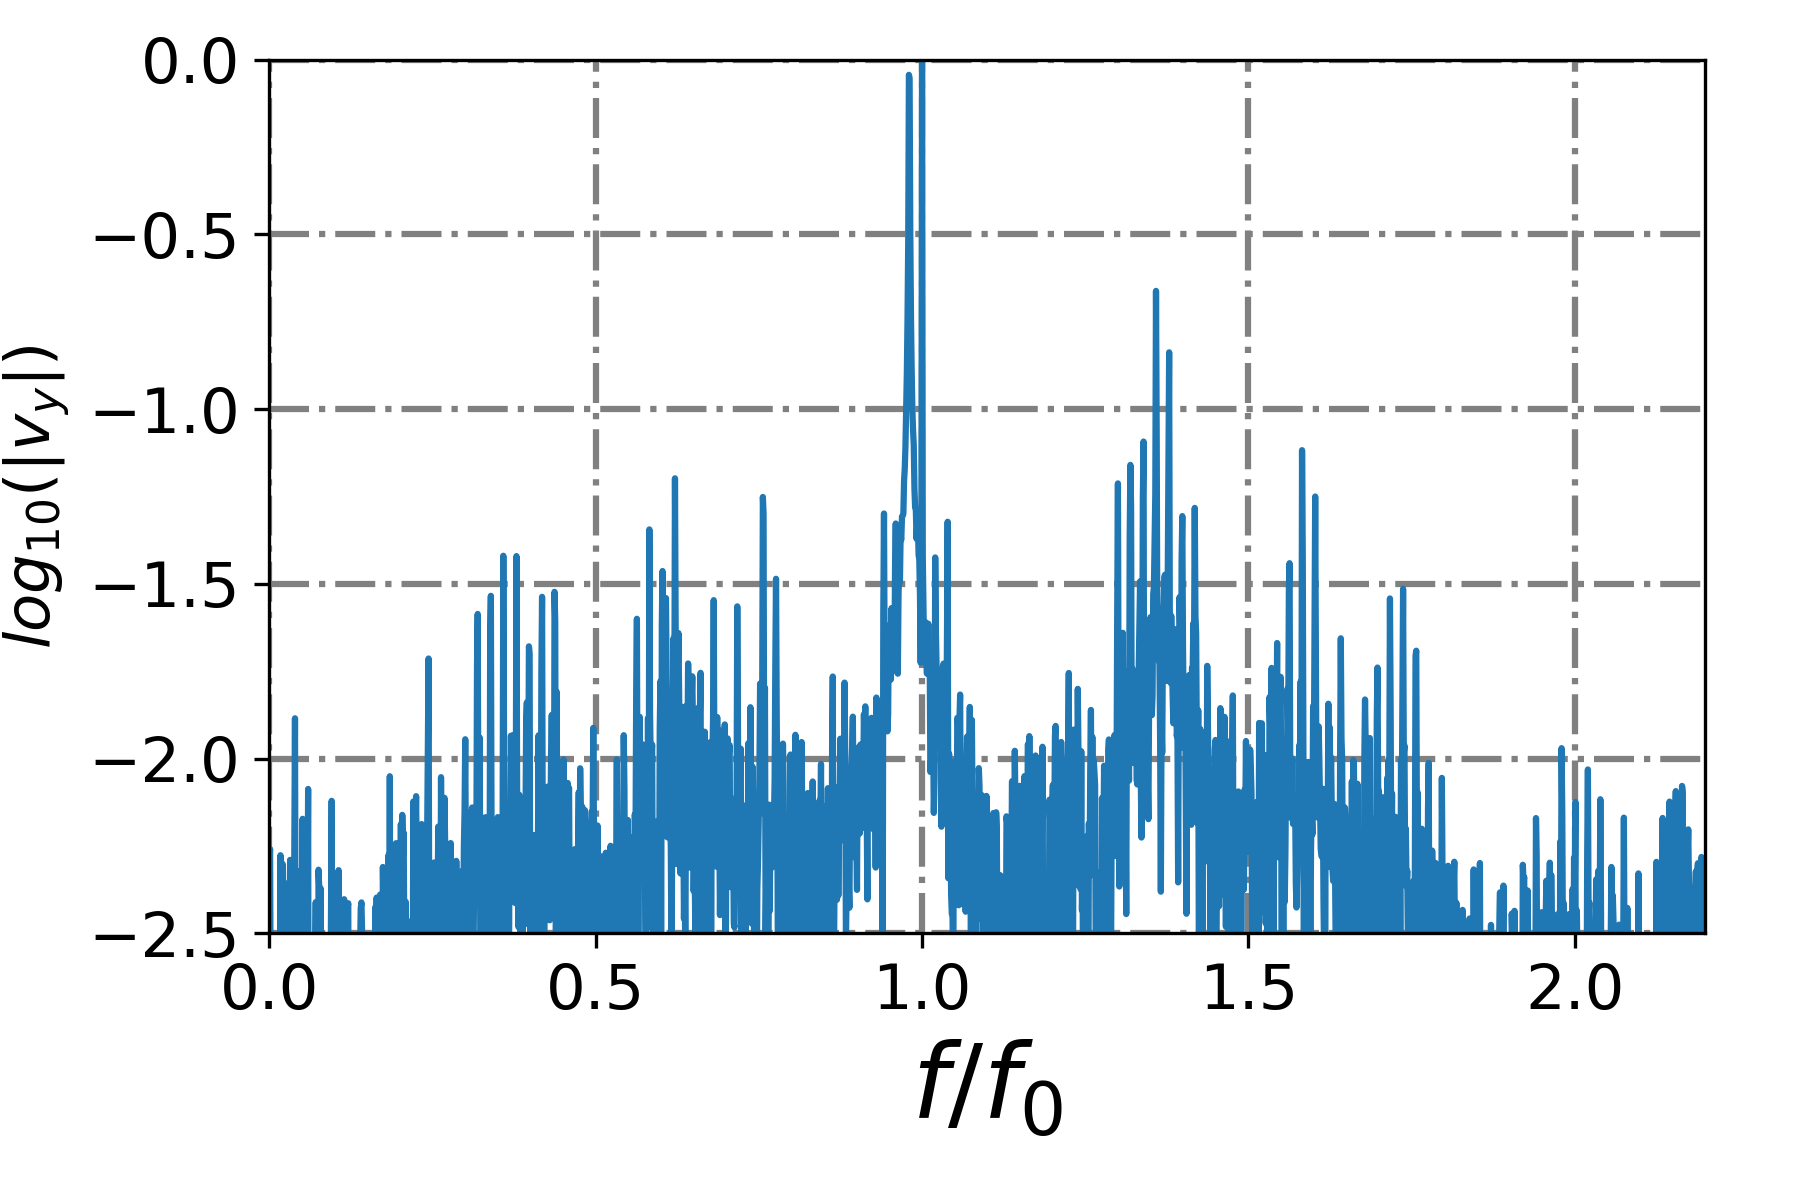
\includegraphics[width=1\textwidth]{pics/H40L60N1ap05dp20w1p63Deltawp02Biharm/spectrumX35p6Y11p2.png}
    \caption{Спектр}
  \end{subfigure}
  \begin{subfigure}[с]{0.45\textwidth}
    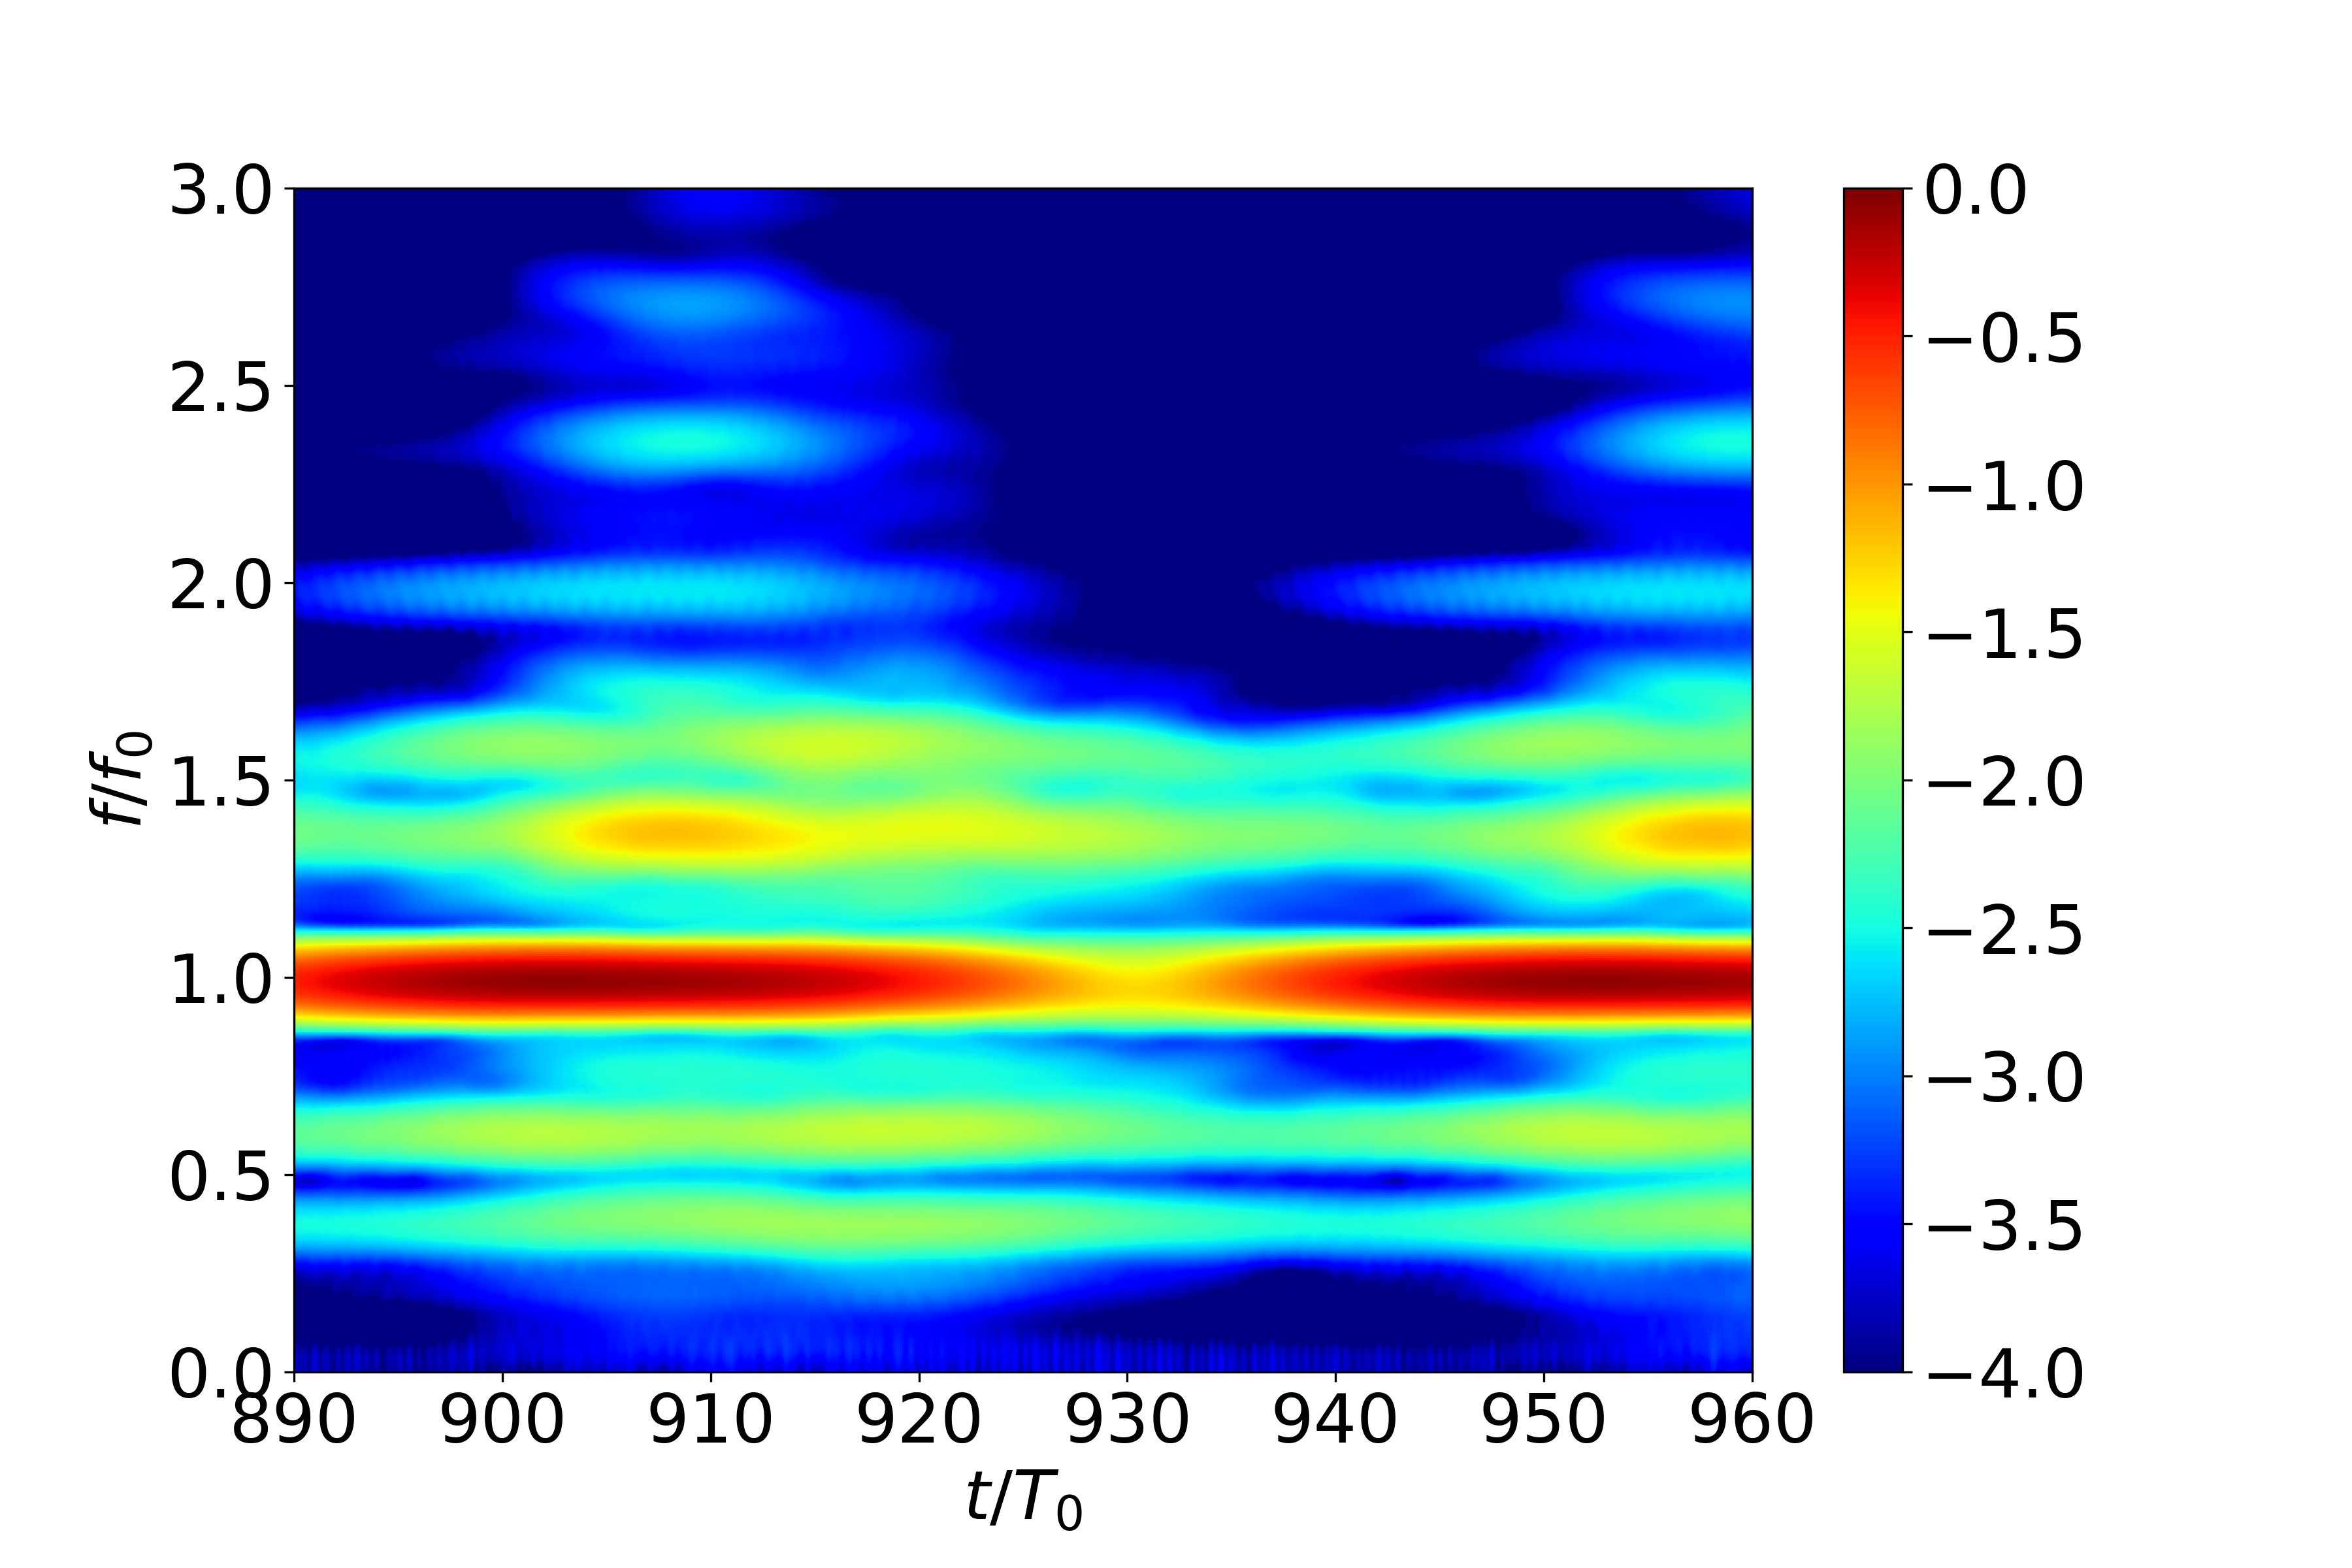
\includegraphics[width=1\textwidth]{pics/H40L60N1ap05dp20w1p63Deltawp02Biharm/TFspectrumX35p6Y11p2N256.png}
    \caption{Частотно-временная диаграмма}
  \end{subfigure}
  \caption{Количественные результаты исследования бигармонического аттрактора внутренних волн с двумя близкими частотами $\omega_1/N=0.628$,  $\omega_2/N=0.641$.}
  \label{fig:biharmVyap005-2}
\end{figure}

Помимо детального анализа результатов моделирования бигармонических аттракторов полученных с помощью метода спектральных элементов, были получены результаты моделирования с помощью метода конечного объема (см. рис. \ref{fig:biharm}). Из рисунка видно, что качественно картина течения совпала с предсказанной при помощи трассировки лучей. 

\begin{figure}
    \centering
    \scalebox{0.95}{
    \begin{tikzpicture}[scale=1.187, z={(-.707,-.5)}]
        \node[anchor=south west,inner sep=0] at (0,0) {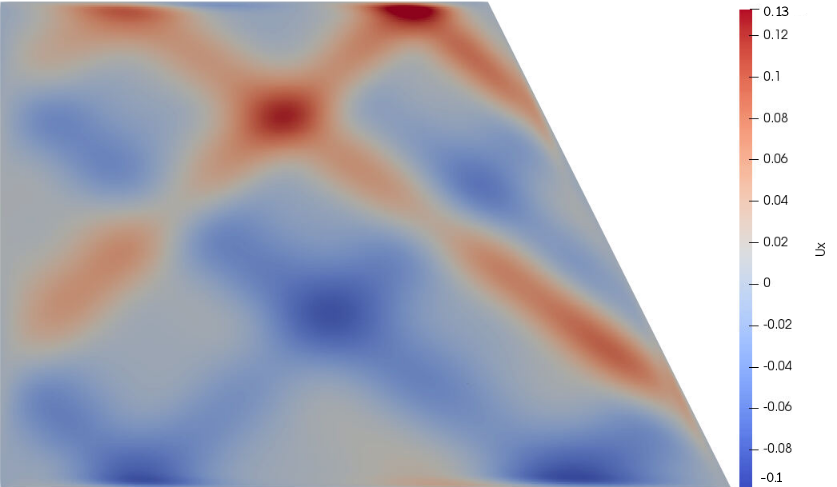
\includegraphics[width=\textwidth]{pics/Biharm.png}};
        \draw (0,0,0) -- (12*0.98,0,0) -- (8*0.98,8*0.98,0)--(0,8*0.98,0) --cycle;
        \draw[style = dashed] (9*0.98,0,0)   -- (0,6.4*0.98,0) -- (2.0*0.98,8*0.98,0) -- (5.65*2*0.98,1.4*0.98,0)-- cycle;
        \draw[style = dashed] (0,0.985*2*0.98,0) -- (6.6*0.98,8*0.98,0) -- (9*0.98,6*0.98,0) -- (2.2*0.98,0,0)  -- cycle;
        \draw[thick,->] (9,6,0) -- (11.1,6,0) node[anchor=north east]{$x$};
        \draw[thick,->] (9,6,0) -- (9.1,8,0) node[anchor=north west]{$z$};
    \end{tikzpicture}
    }
    \caption{Поле горизонтальной компоненты скорости для бигармонического аттрактора и трассировка лучей.}
    \label{fig:biharm}
\end{figure}


\section{Кинетическая энергия для монохроматического и бигармонического режимов}

 Для геометрии, показанной на рис.\ref{fig:domainup}, нижняя и верхняя границы диапазона существования аттрактора соответствуют $\omega_{cr1}/N=0.55$ и $\omega_{cr2}/N=0.74$. При достижении этих критических значений частот происходит вырождение параллелограмма в диагональ трапеции. В качестве интегральной размерной меры эффективности генерации аттрактора при постоянной амплитуде волнопродуктора и неизменной форме резервуара принята кинетическая энергия жидкости, проинтегрированная по площади трапеции $S$: $E_{k}(t)=\int_{S}\frac{\rho_{m}}{2}\left[v_{y}^2(t)+v_{x}^2(t)\right]dS$. Для этой меры можно ввести значение, осредненное в скользящем временном окне по достаточно большому числу периодов колебаний $<E_{k}(t)>$, и вариацию относительно среднего, рассчитываемую как $r=D(E_{k}(t)-<E_{k}(t)>)/<E_{k}(t)>$, где $D(E_{k}(t)-<E_{k}(t)>)$ -- дисперсия относительно среднего. Безразмерные величины $\overline{E}_{k}(t)$ и $<\overline{E}_{k}(t)>$ определены путем нормировки на величину $\rho_{m}S(a\omega)^2/2$. Известно, что режимы движения в аттракторах могут быть близки как к прогрессивным, так и к стоячим волнам ~\cite{Brouzetetal2017}. Величина $r$ позволяет дать количественную оценку близости наблюдаемого режима к одному из этих предельных случаев \cite{Brouzetetal2017}. 


Характерный вид зависимостей, наблюдаемых в монохроматическом режиме при малой амплитуде колебаний показан на 

рис. \ref{fig:domainup}
для  $a=0.02$cм ($a/H=5\cdot 10^{-4}$), $\omega/N=0.63$. Характерное время выхода системы на установившийся режим составляет порядка $30$ периодов колебаний, спектр сигнала является с высокой точностью монохроматическим, колебания кинетической энергии относительно среднего имеют небольшую амплитуду ($r=0.103$). За первую ветвь аттрактора принят пучок с наибольшим значением плотности энергии, возникающий после фокусирующего отражения от наклонной стенки. Величины интегральных параметров, характеризующих линейные монохроматические режимы при фиксированном значении $a/H=5\cdot 10^{-4}$ в частотном диапазоне от $\omega_{cr1}/N=0.55$ до $\omega_{cr2}/N=0.74$ приведены в таблице \ref{tab:bolts002}. Видно, что при фиксированной амплитуде колебаний величина кинетической энергии аттрактора максимальна при $\omega/N=0.63$. Очевидно, что при этом значении частоты возмущающего воздействия следует ожидать сильных нелинейных эффектов при увеличении амплитуды колебаний волнопродуктора. Величина $r$ при $\omega/N=0.63$ достигает минимума: движение в аттракторе представлено прогрессивной волной.  Характерные картины течения и зависимости, наблюдаемые в случае слабонелинейного режима при $\omega/N=0.63$ приведены на рис.\ref{fig:Vyamp05} для $a=0.05$см ($a/H=1.25\cdot 10^{-3}$). В слабонелинейном режиме имеет место триадный резонанс \cite{Dauxoisetal2018}, при котором генерируются две дочерние субгармонические волны малой амплитуды.  Частотно-временная диаграмма, показанная на рис. \ref{fig:Vyamp05}, представляет собой спектр сигнала, вычисленный в скользящем окне и осредненный по окрестности точки, лежащей в середине первой ветви аттрактора. Частотный спектр внутренних волн при данном режиме является дискретным, с доминирующим вкладом, соответствующим частоте возмущения $\omega_{0}$, двумя дочерними субгармоническими частотами $\omega_{1}^{*}+\omega_{2}^{*}=\omega_{0}$, двумя супергармоническими частотам $\omega_{1}^{**}=\omega_{1}^{*}+\omega_{0}$, $\omega_{2}^{**}=\omega_{2}^{*}+\omega_{0}$ и удвоенной частотой $2\omega_{0}$. 


\begin{figure}
	\centering
	\begin{subfigure}[с]{0.45\textwidth}
	    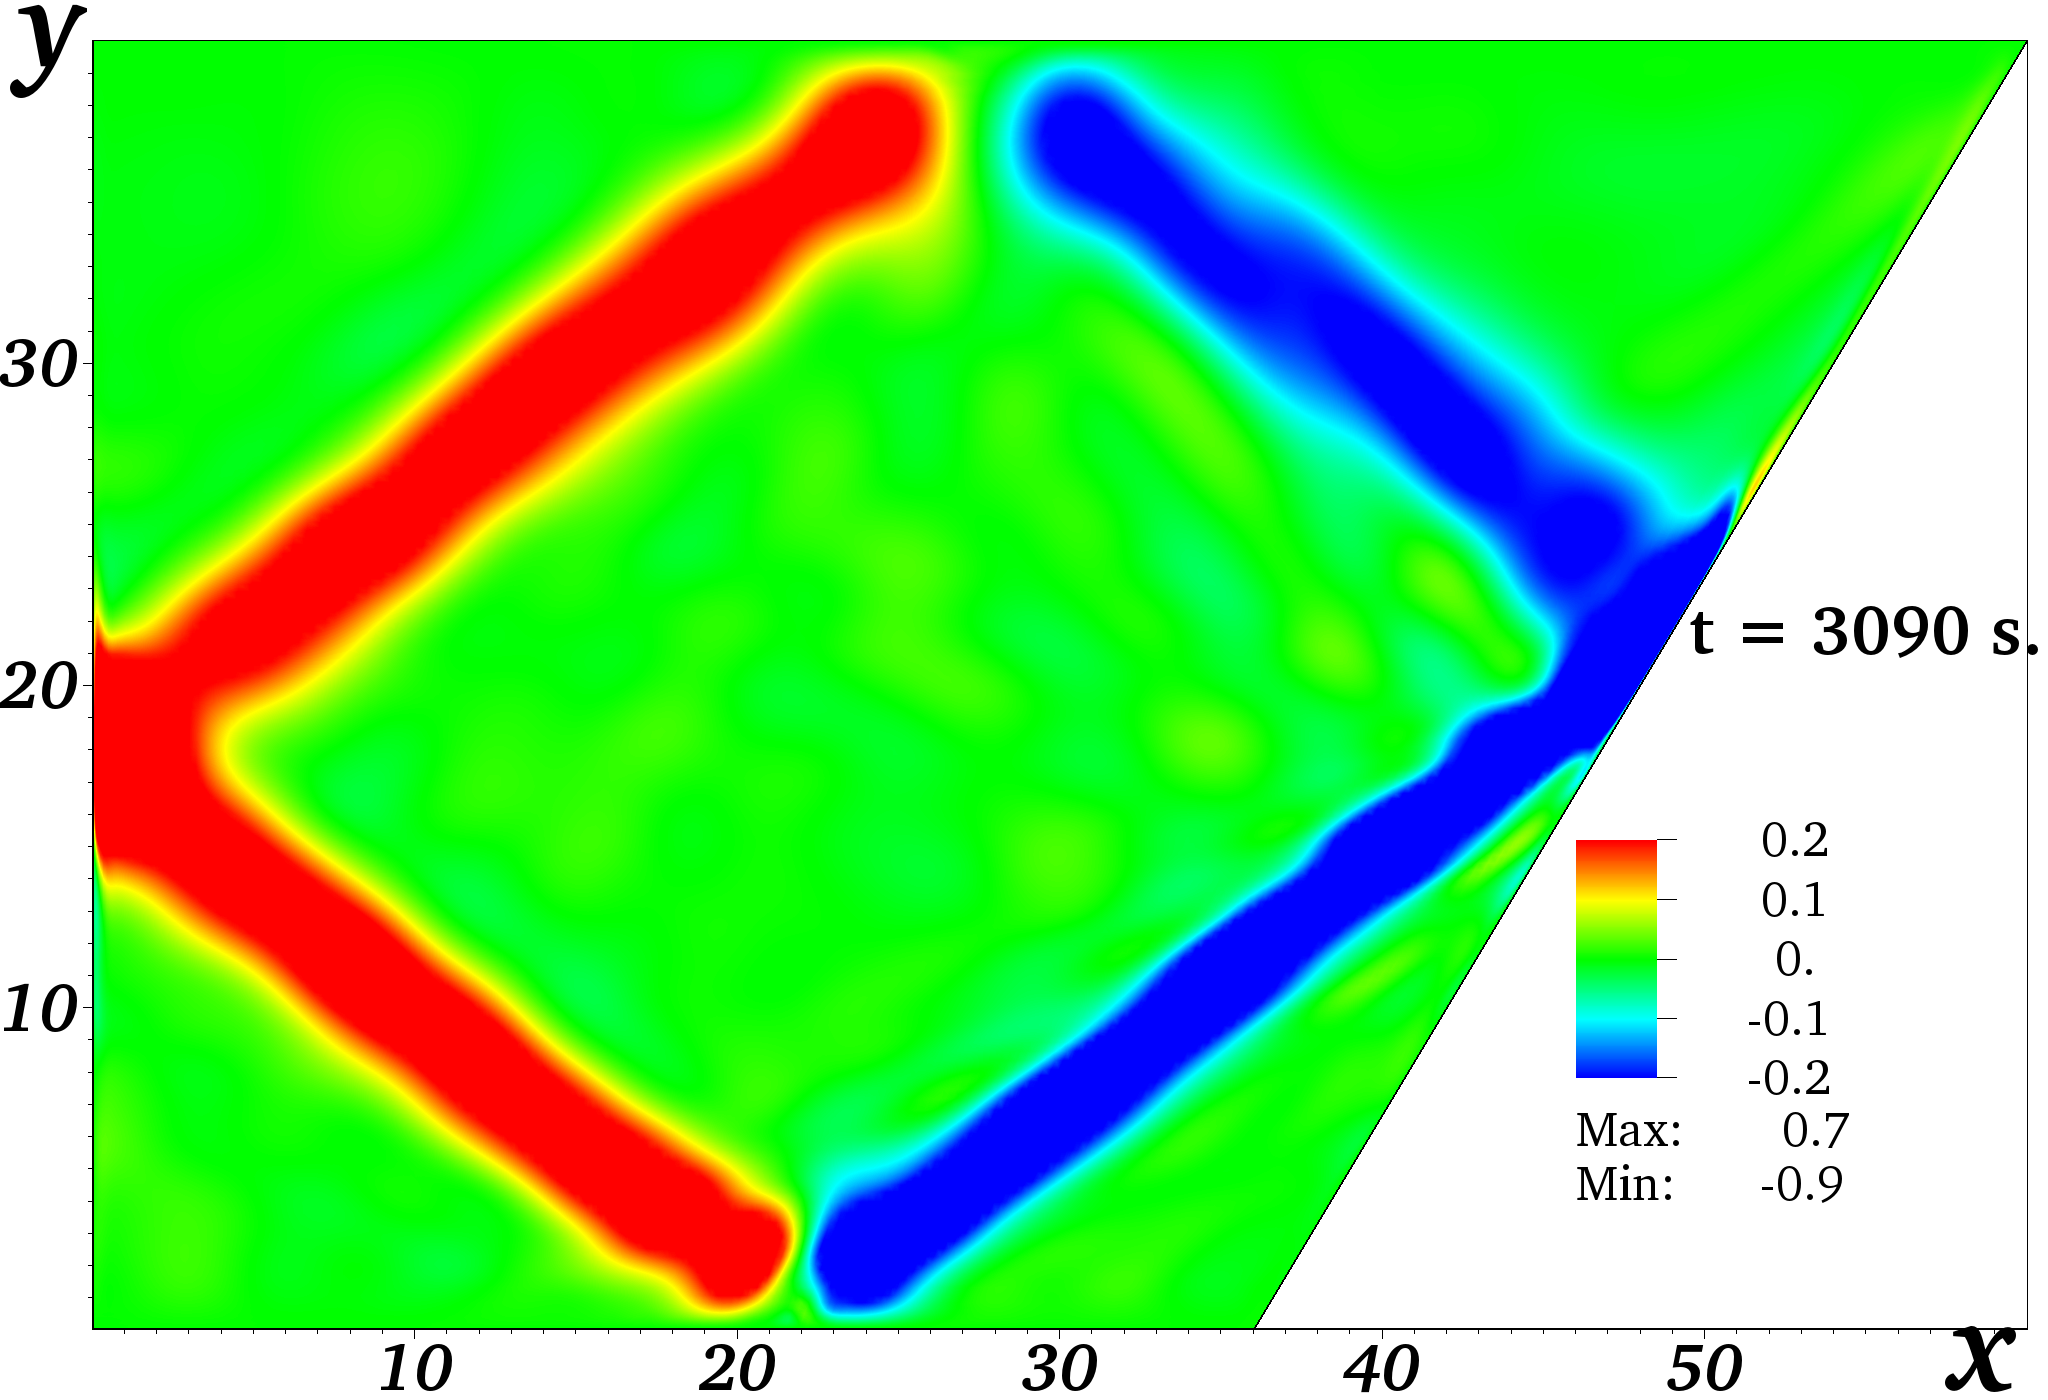
\includegraphics[width=1\textwidth]{pics/H40L60N1ap05dp20w0p63/2D36x36DiagramH40L60N1ap05dp20w0p63Vyn00308.png}
	    \caption{Поле вертикальной компоненты скорости при монохроматическом внешнем воздействии с амплитудой($a/H=5\cdot 10^{-4}$)}
	\end{subfigure}
	\begin{subfigure}[с]{0.45\textwidth}
	    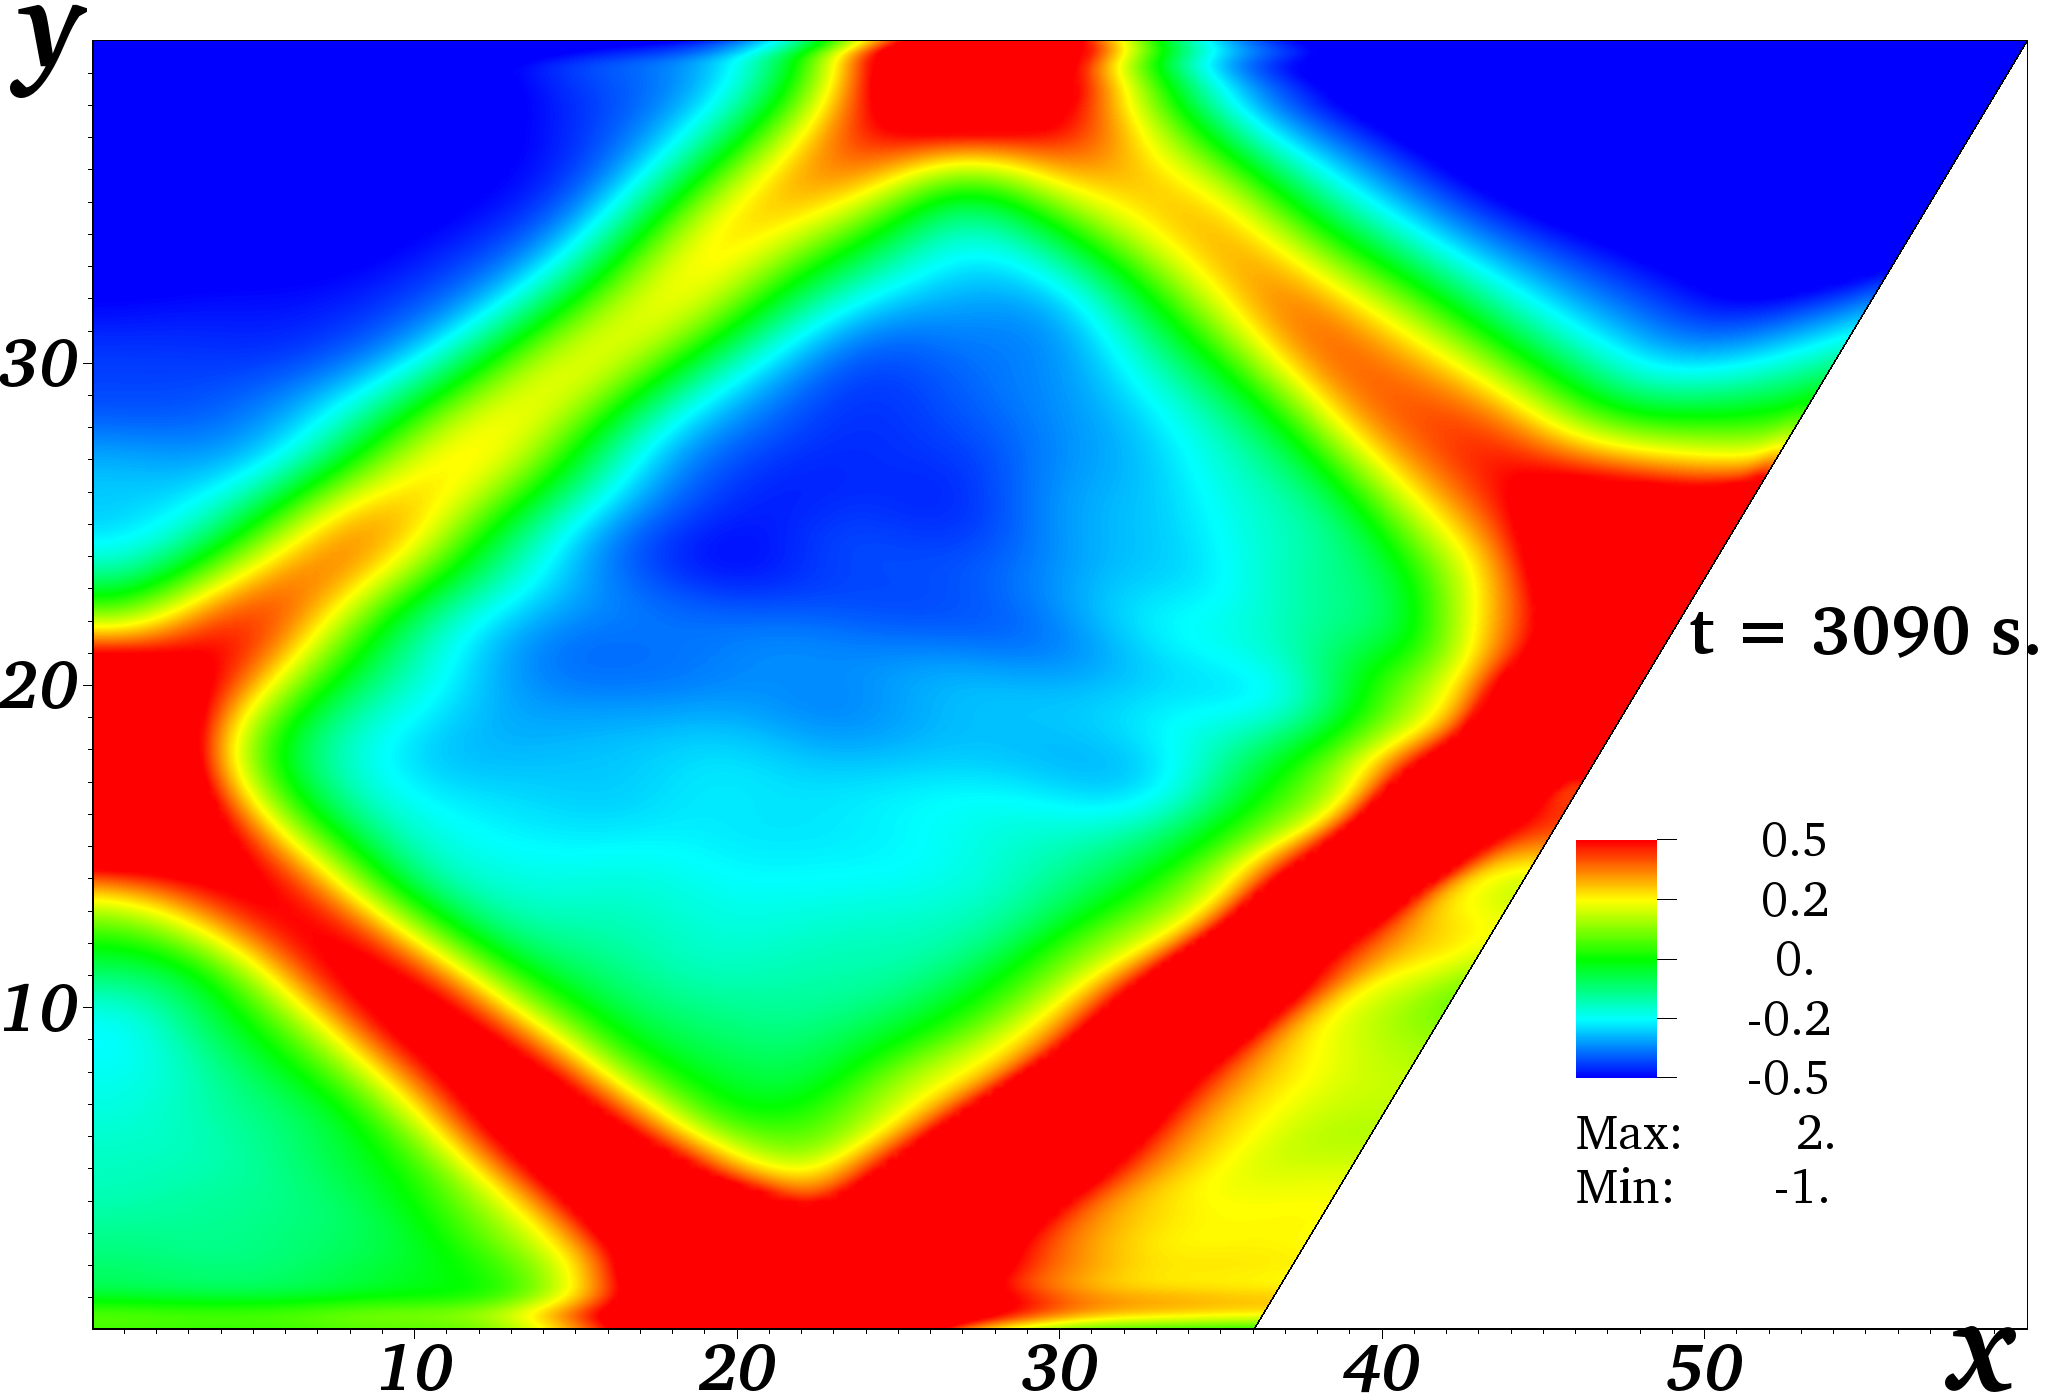
\includegraphics[width=1\textwidth]{pics/H40L60N1ap05dp20w0p63/2D36x36DiagramH40L60N1ap05dp20w0p63Pn00308.png}
	    \caption{Поле давления при монохроматическом внешнем воздействии с амплитудой ($a/H=5\cdot 10^{-4}$)}
	\end{subfigure}
	\par
	\begin{subfigure}[с]{0.45\textwidth}
	    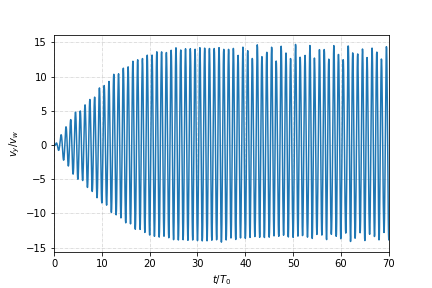
\includegraphics[width=1\textwidth]{pics/H40L60N1ap05dp20w0p63/vyX35p57Y11p27t4400.png}
	    \caption{Скорость в середине первого луча аттрактора}
	\end{subfigure}
	\begin{subfigure}[с]{0.45\textwidth}
	    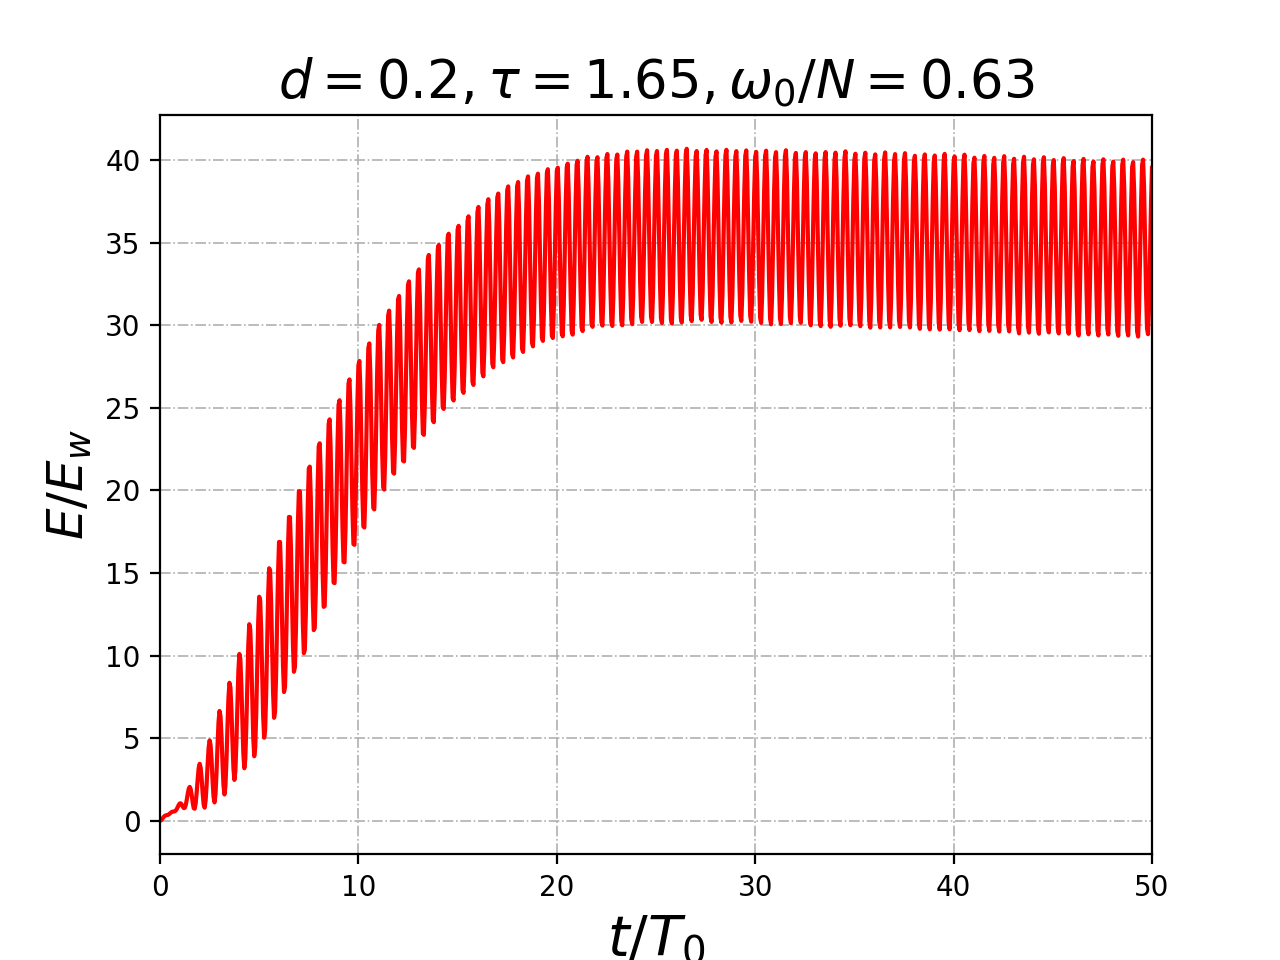
\includegraphics[width=1\textwidth] {pics/H40L60N1ap05dp20w0p63/2D36x36DiagramH40L60N1ap05dp20w0p63totKEnonDim.png}
	    \caption{Кинетическая энергия в середине первого луча аттрактора}
	\end{subfigure}
	\par
	\begin{subfigure}[с]{0.45\textwidth}
	    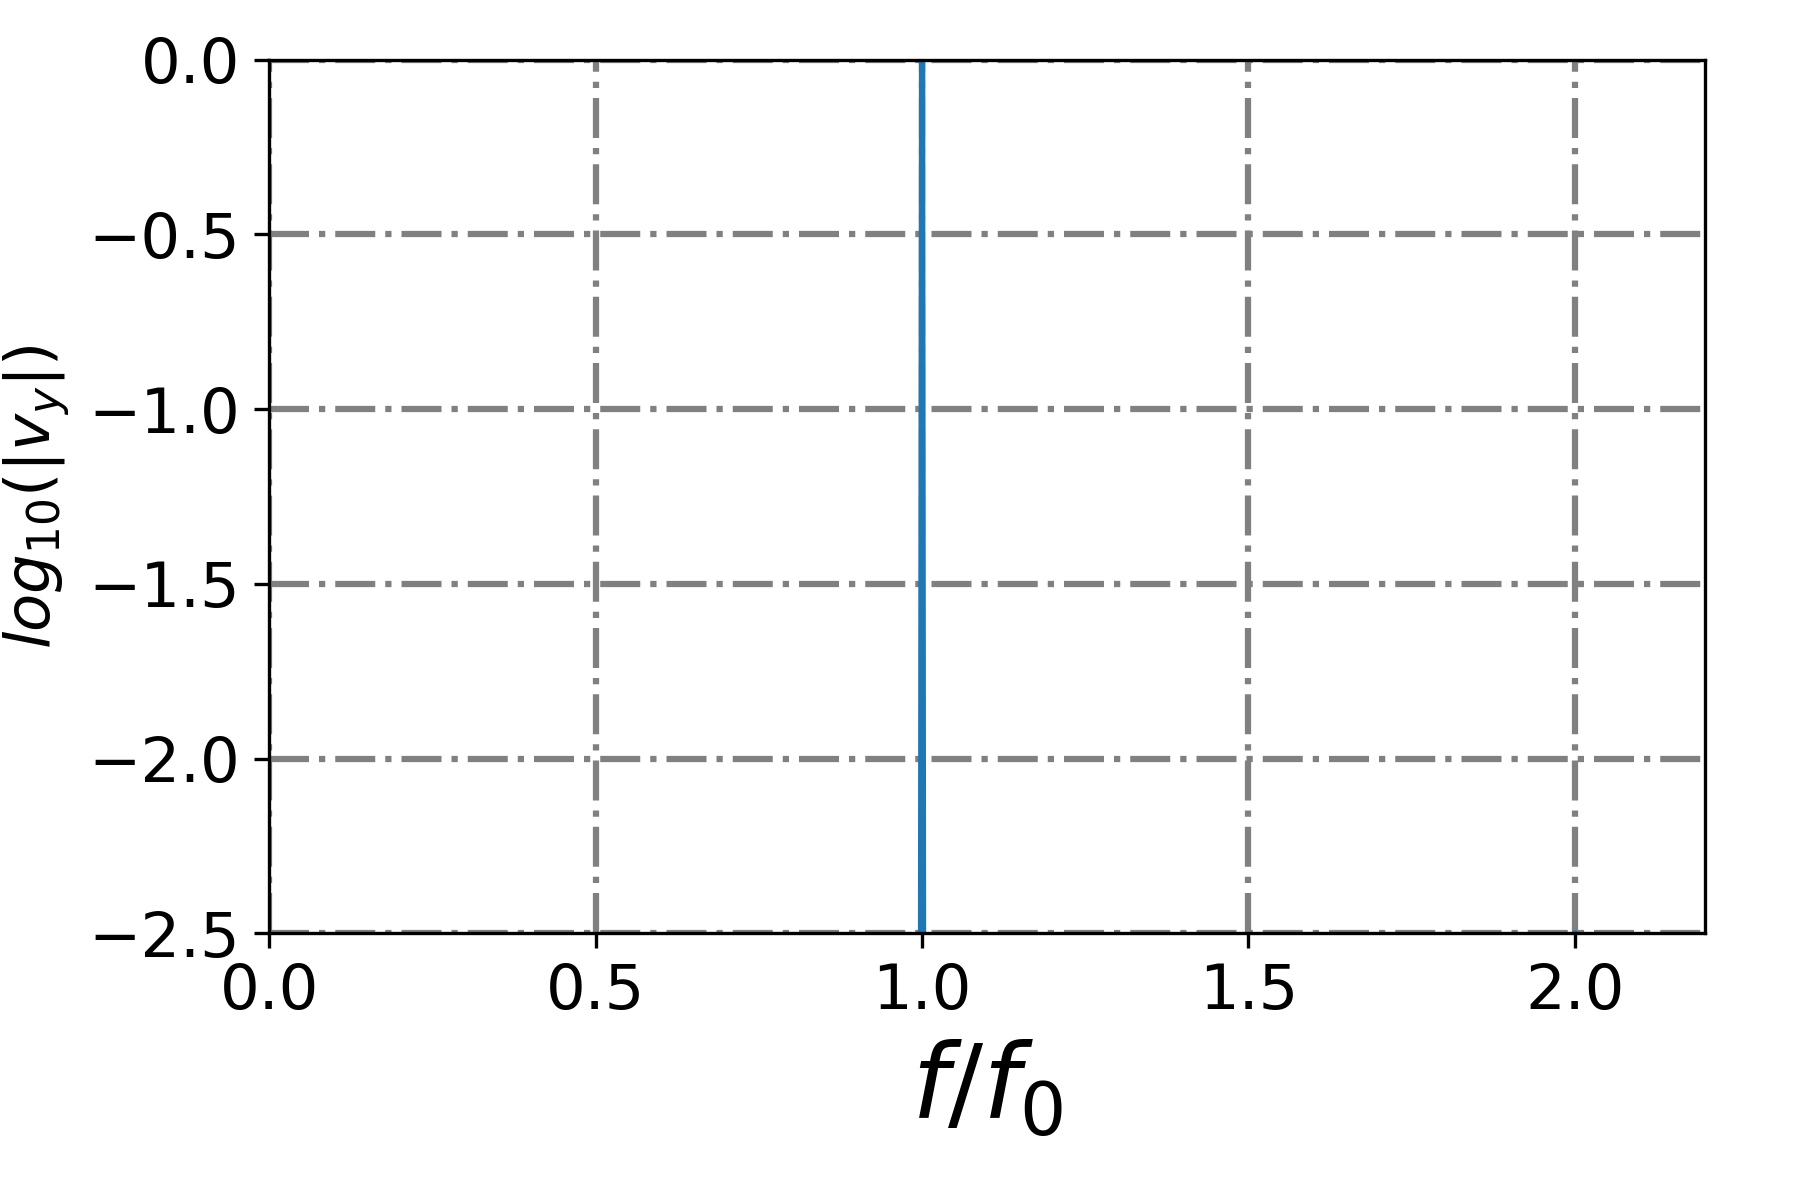
\includegraphics[width=1\textwidth]{{pics/H40L60N1ap05dp20w0p63/spectrumX35.6Y11.2}.png}
	    \caption{Спектр}
	\end{subfigure}
	\begin{subfigure}[с]{0.45\textwidth}
	    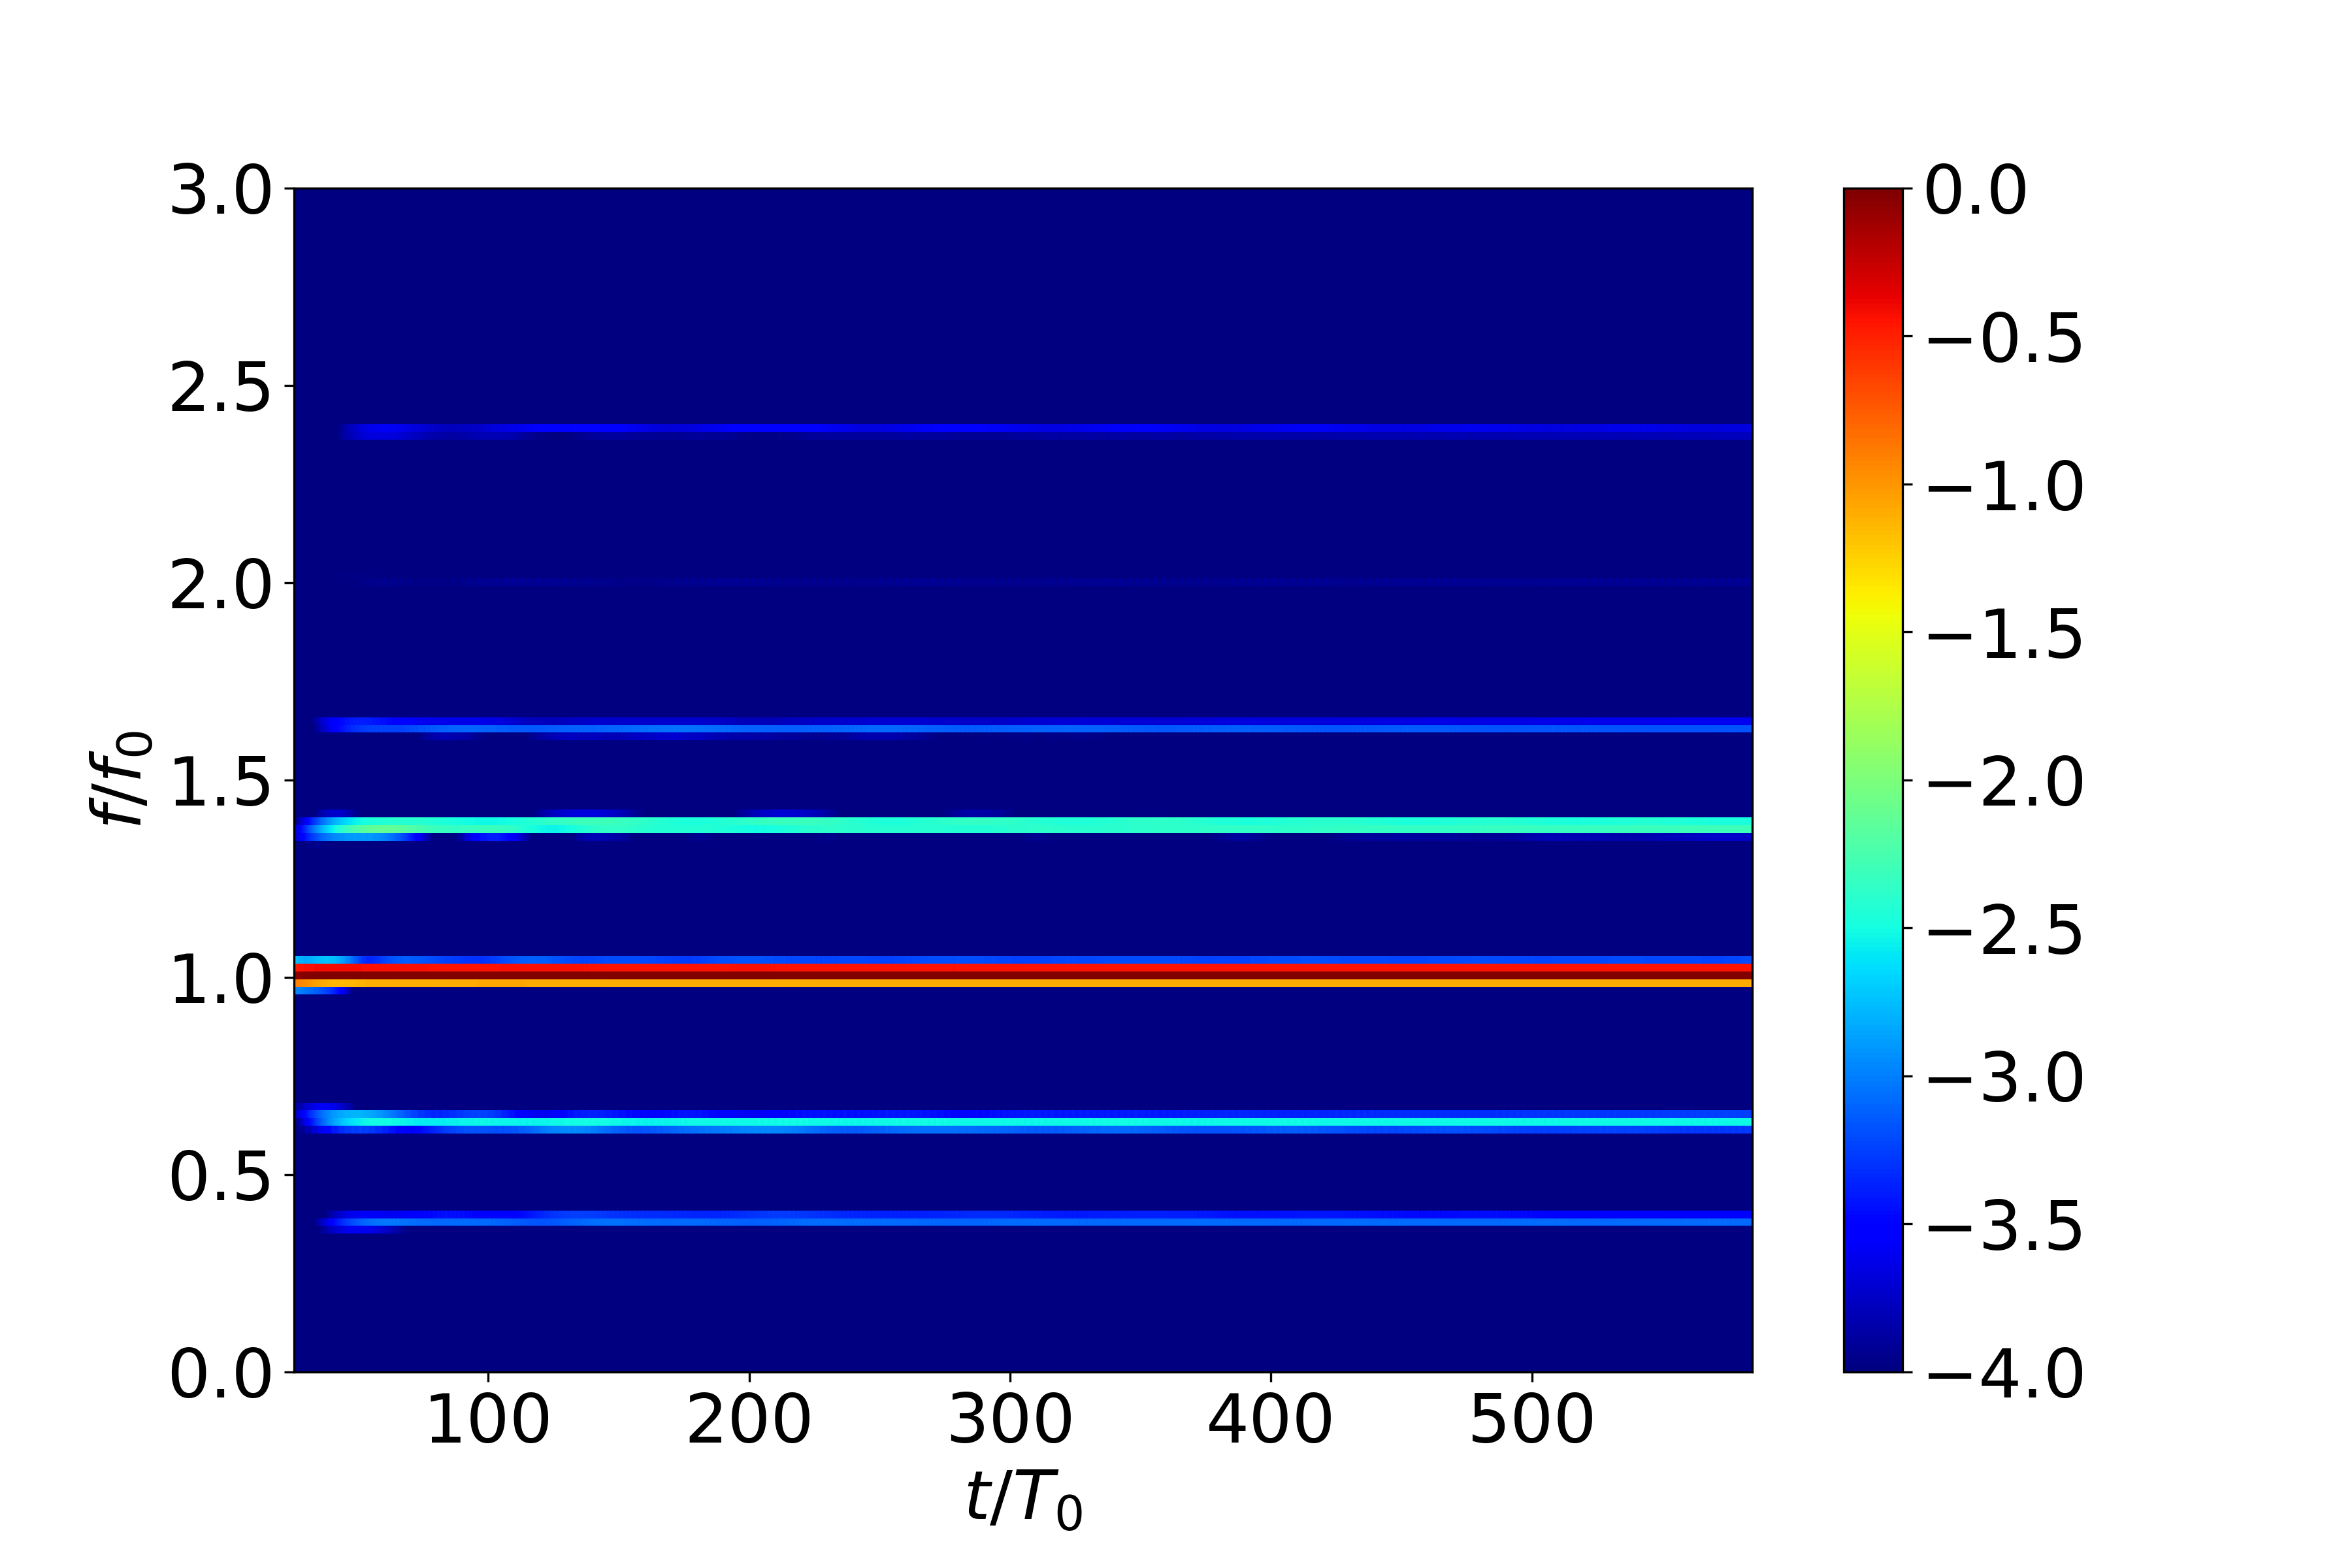
\includegraphics[width=1\textwidth]{{pics/H40L60N1ap05dp20w0p63/TFspectrumX35.6Y11.2N1024}.png}
	    \caption{Частотно-временная диаграмма}
	\end{subfigure}
	\caption{Характерная картина течения при монохроматическом воздействии }
	\label{fig:Vyamp05}
\end{figure}

\begin{table}
	\caption{ Кинетическая энергия при монохроматических воздействиях с амплитудой $a=0.02 cm$}. 
	\begin{center}
		\begin{tabular}{|c|c|c|c|c|c|}
			\hline
			$\displaystyle \frac{\omega_0}{N}$ & $E_k $ &  $<\overline{E}_{k}>$ & r\\
			0.55 ($\omega_{cr,1}$) & $1.32 \cdot 10^{-4}   $& 2.151    & 0.618     \\
			0.58                   & $8.45 \cdot 10^{-4}   $& 12.56    & 0.281     \\
			0.59                   & $ 12  \cdot 10^{-4}   $& 17.33    & 0.3       \\
			0.63                   & $29   \cdot 10^{-4}   $& 36.68    & 0.103     \\
			0.641                  & $23   \cdot 10^{-4}   $& 28.55    & 0.1129    \\
			0.66                   & $13.2 \cdot 10^{-4}   $& 15.14    & 0.152     \\
			0.70                   & $2.84 \cdot 10^{-4}   $& 2.896    & 0.295     \\
			0.74 ($\omega_{cr,2}$) & $1.50 \cdot 10^{-4}   $& 1.356    & 0.215     \\
			\hline
		\end{tabular}
	\end{center}
	\label{tab:bolts002}
\end{table}

При дальнейшем увеличении амплитуды возмущения до $a=0.1$см ($a/H=2.5\cdot 10^{-3}$) происходит развитие каскада триадных взаимодействий. Характерные картины волновых полей, спектров и развития во времени процесса колебаний и кинетической энергии системы приведены на рисунках \ref{fig:Vyamp1}. В частотном спектре сигнала доминируют дискретные компоненты, соответствующие частотам дочерних волн, возникающих при триадном резонансе аналогичные компонентам спектра, возникающим в слабонелинейном случае ($a/H=1.25\cdot 10^{-3}$). При этом полный спектр сигнала представляет собой суперпозицию дискретного и непрерывного спектра. Наличие непрерывного спектра свидетельствует о возникновении режима развитой волновой турбулентности \cite{Brouzet2016,Brouzetetal2017}. Соответствующие характеристики для кинетической энергии системы в сильно нелинейном режиме приведены в таблице \ref{tab:bolts01}. Из сопоставления таблиц \ref{tab:bolts002} и \ref{tab:bolts01} видно, что величины глобальных безразмерных энергетических характеристик системы (средней энергии  $<\overline{E}_{k}>$ и вариации относительно среднего $r$) в случае режима развитой волновой турбулентности слабо отличаются от безразмерных величин, характерных для линейного режима. Сопоставление волновых картин в линейном и нелинейном случаях показывает, что во втором случае энергия более равномерно распределена по изучаемой области: ветви аттрактора имеют большую ширину, а дочерние волны заполняют все пространство.

\begin{table}
	\caption{  Кинетическая энергия при монохроматических воздействиях с амплитудной $a=0.1 cm$. }
	\begin{center}
		\begin{tabular}{|c|c|c|c|c|}
			\hline
			$\displaystyle \frac{\omega_0}{N}$ & $E_k (erg)$ &  $<\overline{E}_{k}>$  & r\\
			%          $a$ &    $\displaystyle \frac{\omega_0}{N}$   & $E_k$ & ${E_k}/{\frac{(a\omega_0)^2}{2}}$ & $D_k$ & r\\
			0.55 ($\omega_{cr,1}$) & $33.0 \cdot 10^{-4}              $& 2.14  & 0.6193     \\
			0.63                   & $725 \cdot 10^{-4}              $& 36.7  & 0.1346     \\
			0.74 ($\omega_{cr,2}$) & $37.0 \cdot 10^{-4}              $& 1.35  & 0.2192     \\
			\hline
		\end{tabular}
	\end{center}
	\label{tab:bolts01}
\end{table}

Характерный пример волновой картины и основных качественных и количественных характеристик системы в линейном случае при бигармоническом внешнем воздействии приведен на рис.\ref{fig:biharmVyamp02} для следующих значений параметров: $\omega_1/N=0.58, \omega_2/N=0.66, a=0.02$см. Видно, что система выходит на режим квазистационарных биений за время порядка $40$ периодов колебаний, что близко к характерному времени выхода на процесс стационарных колебаний в монохроматическом случае. На частотном спектре доминируют пики, соответствующие частотам внешнего возмущения, имеются также пики, соответствующие частоте  $2\omega_1/N$ и разностной частоте $(\omega_2-\omega_1)/N$, но их величина более чем на два порядка меньше основного пика. Моменты времени, соответствующие максимальным значениям кинетической энергии, существенно отстают от моментов времени, соответствующих максимальным значениям амплитуды колебаний волнпродуктора. Важно отметить, что после выхода системы на режим установившихся биений средняя кинетическая энергия системы, возбуждаемой бигармоническим возмущением, с высокой точностью равна сумме энергий аттракторов, возбуждаемых монохроматическими возмущениями по отдельности $\overline{E}_{k}= { 21.7 \cdot 10^{-4}  }\approx \overline{E}_{k1}+\overline{E}_{k2}= (8.45+13.2) \cdot 10^{-4} = 21.65 \cdot 10^{-4}\, (erg/cm^2) $. Таким образом, в линейном режиме с высокой точностью соблюдается принцип линейной суперпозиции, что выполняется также при малой разности частот $(\omega_1-\omega_2)/N$. 

Примеры нелинейной динамики волновых аттракторов, генерируемых бигармоническими колебаниями волнопродуктора приведены на рис. \ref{fig:biharmVyap005-1} %\ref{fig:biharmVyap005-1-1} 
($\omega_1/N=0.66$, $\omega_2/N=0.628$, $\delta \omega/N=0.031$) и \ref{fig:biharmVyap005-2}, 
%\ref{fig:biharmVyap005-2-1} 
($\omega_1/N=0.628$, $\omega_2/N=0.641$, $\delta \omega/N=0.013$). Во всех случаях амплитуды колебаний волнопродуктора составили $a_{1}=a_{2}=0.05$см. Можно видеть, что в обоих случаях формируется движение, для которого характерен сложный частотный спектр, причем при уменьшении расстройки частот $\delta \omega$ наблюдается тенденция к более густому <<заселению>> спектра.  На графиках зависимости вертикальной скорости от времени виден характерный процесс <<биений>>. График зависимости кинетической энергии системы от времени показывает, что помимо колебаний среднего значения энергии имеет место нетривиальная динамика высокочастотных пульсаций энергии: на фазах роста и убывания огибающей амплитуды колебаний волнопродуктора амплитуды пульсаций могут отличаться на порядок. Таким образом, для нелинейного бигармонического режима характерны периодические <<вспышки>> волновой турбулентности. Такие <<вспышки>> хорошо видны на частотно-временных диаграммах, приведенных на рис.  \ref{fig:biharmVyap005-1} и \ref{fig:biharmVyap005-2}. В частности, на частотно-вереиенной диаграмме, приведенной на рис.  \ref{fig:biharmVyap005-1}, можно видеть, что <<биения>> амплитуды сигнала на частоте, близкой к частоте возмущающего воздействия, сдвинуты по времени относительно <<биений>> дочерних волн. Таким образом, <<биения>> огибающей колебаний волнопродуктора, <<биения>> средней кинетической энергии и <<вспышки>> волновой турбулентности рассогласованны между собой по времени. Можно предположить, что и в природных системах имеется рассогласование по времени между огибающей амплитуды внутреннего прилива и интенсификацией внутренней волновой турбулентности и перемешивания. Предварительное исследование энергии аттракторов, генерируемых бигармоническим возмущением, показывает, что в нелинейном случае средняя энергия системы существенным образом отличается от суммы энергий составляющих.  
